\documentclass[11pt]{book}

%%%%%%%%%%%%%%Include Packages%%%%%%%%%%%%%%%%%%%%%%%%%%
\usepackage{xcolor}
\usepackage{mathtools}
\usepackage[a4paper, total={6in, 8in}, margin=1.25in]{geometry}
\usepackage{amsmath}
\usepackage{amssymb}
\usepackage{paralist}
\usepackage{rsfso}
\usepackage{amsthm}
\usepackage{wasysym}
\usepackage[inline]{enumitem}   
\usepackage{hyperref}
\usepackage{tocloft}
\usepackage{wrapfig}
\usepackage{titlesec}
\usepackage{colortbl}
\usepackage{stackengine} 
%%%%%%%%%%%%%%%%%%%%%%%%%%%%%%%%%%%%%%%%%%%%%%%%%%%%%%%%


%%%%%%%%%%%%%%%Chapter Setting%%%%%%%%%%%%%%%%%%%%%%%%%%
\definecolor{gray75}{gray}{0.75}
\newcommand{\hsp}{\hspace{20pt}}
\titleformat{\chapter}[hang]{\Huge\bfseries}{\thechapter\hsp\textcolor{gray75}{$\mid$}\hsp}{0pt}{\Huge\bfseries}
%%%%%%%%%%%%%%%%%%%%%%%%%%%%%%%%%%%%%%%%%%%%%%%%%%%%%%%%

%%%%%%%%%%%%%%%%%Theorem environments%%%%%%%%%%%%%%%%%%%
\newtheoremstyle{break}
  {\topsep}{\topsep}%
  {\itshape}{}%
  {\bfseries}{}%
  {\newline}{}%
\theoremstyle{break}
\theoremstyle{break}
\newtheorem{axiom}{Axiom}
\newtheorem{thm}{Theorem}[section]
\renewcommand{\thethm}{\arabic{section}.\arabic{thm}}
\newtheorem{lem}{Lemma}[thm]
\newtheorem{prop}[lem]{Proposition}
\newtheorem{corL}{Corollary}[lem]
\newtheorem{corT}[lem]{Corollary}
\newtheorem{defn}{Definition}[corL]
\newenvironment{indEnv}[1][Proof]
  {\proof[#1]\leftskip=1cm\rightskip=1cm}
  {\endproof}
%%%%%%%%%%%%%%%%%%%%%%%%%%%%%%%%%%%%%%%%%%%%%%%%%%%%%%


%%%%%%%%%%%%%%%%%%%%%%%Integral%%%%%%%%%%%%%%%%%%%%%%%
\def\upint{\mathchoice%
    {\mkern13mu\overline{\vphantom{\intop}\mkern7mu}\mkern-20mu}%
    {\mkern7mu\overline{\vphantom{\intop}\mkern7mu}\mkern-14mu}%
    {\mkern7mu\overline{\vphantom{\intop}\mkern7mu}\mkern-14mu}%
    {\mkern7mu\overline{\vphantom{\intop}\mkern7mu}\mkern-14mu}%
  \int}
\def\lowint{\mkern3mu\underline{\vphantom{\intop}\mkern7mu}\mkern-10mu\int}
%%%%%%%%%%%%%%%%%%%%%%%%%%%%%%%%%%%%%%%%%%%%%%%%%%%%%%



\newcommand{\R}{\mathbb{R}}
\newcommand{\N}{\mathbb{N}}
\newcommand{\Z}{\mathbb{Z}}
\newcommand{\Q}{\mathbb{Q}}
\newcommand{\C}{\mathbb{C}}
\newcommand{\T}{\mathcal{T}}
\newcommand{\M}{\mathcal{M}}
\newcommand{\Symm}{\text{Symm}}
\newcommand{\Alt}{\text{Alt}}
\newcommand{\Int}{\text{Int}}
\newcommand{\Bd}{\text{Bd}}
\newcommand{\Power}{\mathcal{P}}
\newcommand{\ee}[1]{\cdot 10^{#1}}
\newcommand{\spa}{\text{span}}
\newcommand{\sgn}{\text{sgn}}
\newcommand{\degr}{\text{deg}}
\newcommand{\pd}{\partial}
\newcommand{\that}[1]{\widetilde{#1}}
\newcommand{\lr}[1]{\left(#1\right)}
\newcommand{\vmat}[1]{\begin{vmatrix} #1 \end{vmatrix}}
\newcommand{\bmat}[1]{\begin{bmatrix} #1 \end{bmatrix}}
\newcommand{\pmat}[1]{\begin{pmatrix} #1 \end{pmatrix}}
\newcommand{\rref}{\xrightarrow{\text{row\ reduce}}}
\newcommand{\txtarrow}[1]{\xrightarrow{\text{#1}}}
\newcommand\oast{\stackMath\mathbin{\stackinset{c}{0ex}{c}{0ex}{\ast}{\Circle}}}


\newcommand{\note}{\color{red}Note: \color{black}}
\newcommand{\remark}{\color{blue}Remark: \color{black}}
\newcommand{\example}{\color{green}Example: \color{black}}
\newcommand{\exercise}{\color{green}Exercise: \color{black}}

%%%%%%%%%%%%%%%%%%%%%%Roman Number%%%%%%%%%%%%%%%%%%%%%%%
\makeatletter
\newcommand*{\rom}[1]{\expandafter\@slowromancap\romannumeral #1@}
\makeatother
%%%%%%%%%%%%%%%%%%%%%%%%%%%%%%%%%%%%%%%%%%%%%%%%%%%%%%%%%

%%%%%%%%%%%%table of contents%%%%%%%%%%%%%%%%%%%%%%%%%%%%
\setlength{\cftchapindent}{0em}
\cftsetindents{section}{2em}{3em}

\renewcommand\cfttoctitlefont{\hfill\huge\bfseries}
\renewcommand\cftaftertoctitle{\hfill\mbox{}}

\setcounter{tocdepth}{2}
%%%%%%%%%%%%%%%%%%%%%%%%%%%%%%%%%%%%%%%%%%%%%%%%%%%%%%%%%


%%%%%%%%%%%%%%%%%%%%%Footnotes%%%%%%%%%%%%%%%%%%%%%%%%%%%
\newcommand\blfootnote[1]{%
  \begingroup
  \renewcommand\thefootnote{}\footnote{#1}%
  \addtocounter{footnote}{-1}%
  \endgroup
}
%%%%%%%%%%%%%%%%%%%%%%%%%%%%%%%%%%%%%%%%%%%%%%%%%%%%%%%%%

%%%%%%%%%%%%%%%%%%%%%Section%%%%%%%%%%%%%%%%%%%%%%%%%%%%%
\makeatletter
\def\@seccntformat#1{%
  \expandafter\ifx\csname c@#1\endcsname\c@section\else
  \csname the#1\endcsname\quad
  \fi}
\makeatother
%%%%%%%%%%%%%%%%%%%%%%%%%%%%%%%%%%%%%%%%%%%%%%%%%%%%%%%%%

%%%%%%%%%%%%%%%%%%%%%%%%%%%%%%%%%%%Enumerate%%%%%%%%%%%%%%
\makeatletter
% This command ignores the optional argument 
% for itemize and enumerate lists
\newcommand{\inlineitem}[1][]{%
\ifnum\enit@type=\tw@
    {\descriptionlabel{#1}}
  \hspace{\labelsep}%
\else
  \ifnum\enit@type=\z@
       \refstepcounter{\@listctr}\fi
    \quad\@itemlabel\hspace{\labelsep}%
\fi}
\makeatother
\parindent=0pt
%%%%%%%%%%%%%%%%%%%%%%%%%%%%%%%%%%%%%%%%%%%%%%%%%%%%%%%%%%



\begin{document}

	\begin{titlepage}
		\begin{center}
			\vspace*{1cm}
			\Huge \color{red}
				\textbf{Class Notes}\\
			\vspace{0.5cm}			
			\Large \color{black}
				Math 654 - Introduction to Fluid Dynamics\\
				Professor Silas Alben\\	
				University of Michigan\\
			\vspace{2cm}

			
\includegraphics[scale=0.95]{hmm.pdf}
			
			
			\vspace{4cm}
			\LARGE
				\textbf{Jinyan Miao}\\
				\large \textbf{and his friends from UMich Honors Math}\\
				\hfill\break
				\LARGE Fall 2022\\
			\vspace{1cm}

		\vspace*{\fill}
		\end{center}			
	\end{titlepage}

\newpage 
\tableofcontents
\addtocontents{toc}{~\hfill\textbf{Page}\par}

\newpage
\setcounter{page}{1}
\vspace*{\fill}


\newpage
\chapter{Fluid Flow}
In this text, assuming Cartesian coordinate system, a point in $3$-dimensional space is usually denoted as $(x,y,z)$, and a point in $4$-dimensional space is usually denoted as $(x,y,z,t)$. Here $(x,y,z)$ represents the location in space, and $t$ is the time dependent variable. Now first we want to find some ways to describe a fluid in such $4$-dimensional space. Note that cylindrical or spherical coordinate system are also used in some cases.\\


\section[Descriptions of Fluid Flow]{\color{red}Description of Fluid Flow\color{black}}

\begin{defn}
The most usual way to describe fluid flow is through the velocity field, which is usually denoted as the following:
\begin{align}
\vec{u}(\vec{x}, t) = (u(\vec{x},t),v(\vec{x},t),w(\vec{x},t))
\end{align}
where $\vec{x}$ is the position vector and $t$ is the time variable. \\
For Cartesian coordinate system, one can write $\vec{x} = (x,y,z)$\\
\end{defn}


\begin{defn}
A steady flow is a fluid with velocity field $\vec{u}(\vec{x}, t)$ that satisfies:
\begin{align}
\frac{\partial \vec{u}}{\partial t} = 0 
\end{align}
in which case we get $\vec{u}$ simplified as $\vec{u}(\vec{x})$. 
\end{defn}


\example For a $2-$dimensional flow, one can write $\vec{u} =(v(x,y,t),\ w(x,y,t), \ 0)$.\\

There are three common visualization methods for fluid flow: \\
(1) streamlines, (2) streaklines, and (3) pathlines. \\

Streamlines are lines that are locally tangent to the velocity field $\vec{u} = (u,v,w)$ at a given instant $t$. Mathematically, a streamline is given by a parametric curve $\vec{a}(s)$ defined by using parametric variable $s$, with position denoted as $(x(s), y(s), z(s))$,
\begin{align}
\vec{a}(s) = \bmat{x(s) \\ y(s) \\ z(s)}
\end{align}
such that $\vec{a}$ satisfies the following:
\begin{align}
\frac{d\vec{a}}{ds} = \bmat{\frac{dx}{ds} \\ \frac{dy}{ds}\\ \frac{dz}{ds}} = c(s) \bmat{u(x(s),y(s),z(s),t)\\ v(x(s),y(s),z(s),t) \\ w(x(s),y(s),z(s),t)}
\end{align}
where $c$ is a scalar function of $s$. \\


A streakline can be considered as dye released from a fixed point in the velocity field. \\
A pathline is a path traced out by a freely moving fluid particle in the velocity field. \\

\example Consider we have a velocity field $\vec{u} (\vec{x},t) = (1,xt)$ where $\vec{x} = (x,y)$.\\

Then we can model the streamlines as $\vec{a}(s)=(x(s),y(s),z(s))$ such that equation (1.4) holds with $c(s) = 1$, and we get:
\begin{align*}
\frac{dx}{ds} = 1\qquad \frac{dy}{ds} = xt \tag{*}
\end{align*}
Solving equation (*) we get:
\begin{align*}
x = s+\bar{x} \qquad\Rightarrow\qquad \frac{dy}{ds} = (s+\bar{x}) t  \qquad\Rightarrow\qquad y= \frac{s^2}{2}t + s\bar{x}t + \bar{y}
\end{align*}
where $\bar{x}, \bar{y}$ are defined by initial condition of the streamline. \\
Here we see that the streamlines are parabolas with curvatures that increase in time. \\

For pathlines, we want to model the path $\vec{a}(t,t_0) = (x(t),y(t))$ of a freely moving particle in the velocity field. Suppose the particle is at position $\vec{x}_0 = (x_0, y_0)$ at time $t_0=0$ with velocity defined by the velocity field at that instance at that position, we can model:
\begin{align*}
\frac{d \vec{a}(t,t_0)}{dt} = \vec{u}(\vec{a}(t,t_0) , t) \qquad \text{where}\qquad \vec{a}(t_0,t_0) = \vec{x}_0
\end{align*}
Here we have:
\begin{align*}
\frac{dx}{dt} = 1\qquad \frac{dy}{dt} =xt
\end{align*}
Solving we get:
\begin{align*}
x = t+x_0\qquad y=\frac{t^3}{3}+x_0\frac{t^2}{2} + y_0
\end{align*}

\hfill\break
For streaklines, suppose the dye is released at time $t_0$ and is stopped releasing at time $\tau_1$, the dye is released at point $\vec{x}_1 = (x_1,y_1)$, define $\tau_0 \leq \tau \leq \tau_1$, we can model the dye as $\vec{a}(t,\tau)=(x(t),y(t))$ that satisfies the following:
\begin{align*}
\frac{d\vec{a}(t,\tau)}{dt} = \vec{u}(\vec{a}(t,\tau),t) \qquad \vec{a}(\tau,\tau) = \vec{x}_1
\end{align*}
Solving for the streaklines in the example, we get:
\begin{align*}
\frac{dx}{dt} = 1 \qquad \frac{dy}{dt} = xt
\end{align*}
\begin{align*}
x = t+x_1 - \tau \qquad \frac{dy}{dt} = (t+x_1 - \tau) t \qquad y = \frac{t^3}{3}+(x_1 -\tau) \frac{t^2}{2} - \frac{\tau^3}{3} - (x_1 - \tau) \frac{\tau^2}{2} + y_1
\end{align*}


\newpage
Material derivative, denoted as $\frac{D}{Dt}$, is the rate of change of a quantity when following a fluid particle, such quantity can be temperature, velocity, concentration of some material, density, energy, and so on. Here we call a quantity $f(x,y,z,t)$, where $x,y,z$ are fluid particle position at time $t$ because we are moving along the fluid, that is, we can write $f(x(t),y(t),z(t),t)$ instead. Here we can write:
\begin{align*}
\frac{Df}{Dt} = \frac{\partial f}{\partial x} \cdot \frac{\partial x}{\partial t} + \frac{\partial f}{\partial	y}\cdot \frac{\partial y}{\partial t} + \frac{\partial f}{\partial z}\cdot \frac{\partial z}{\partial t} + \frac{\partial f}{\partial t} = \frac{\partial f}{\partial t} + (\vec{u}\cdot \nabla) f
\end{align*} 

If we have $\frac{Df}{Dt} = 0$, then we say $f$ is conserved for a fluid particle. \\

\example \\
Acceleration of a fluid is the material derivative of the velocity field of the fluid:
\begin{align*}
\frac{D\vec{u}}{Dt} = \frac{\partial \vec{u}}{\partial t} + (\vec{u} \cdot \nabla) \vec{u}
\end{align*}




\begin{defn}
A fluid is said to be ideal provided that the followings hold:
\begin{enumerate}[topsep=3pt,itemsep=-1ex,partopsep=1ex,parsep=1ex]
\item The fluid is incompressible, the volume of fluid particles is conserved in time.
\item The density of the fluid is constant.
\item The only force acting on the fluid is the fluid pressure, there is no viscosity.
\end{enumerate}
\end{defn}
\begin{defn}
For a fluid, $\vec{n}$ usually denotes the normal vector for geometrical surface within the fluid, pointing outwards, $S$ usually denotes a geometrical surface within the fluid, and $V$ usually denotes a geometrical volume with the fluid. 
\end{defn}

\begin{defn}
Pressure, denoted as $p$, is a force per unit area exerted normal to a geometrical surface element $\vec{n}\, \delta S$ within a fluid due to collisions of fluid molecules. The force exerted on the fluid into which $\vec{n}$ is pointing by the fluid on the other side of $\delta S$ is given by $p\vec{n}\, \delta S$. 
\end{defn}

\example For ideal gas, we have:
\begin{align}
pV = nRT
\end{align}
or in another form:
\begin{align}
p = \rho \frac{R}{M}T
\end{align}
and $M$ is the molar mass of the gas. 



\newpage
\section[Conservation Laws]{\color{red}Conservation Laws\color{black}}
\textbf{Conservation of Mass and Incompressibility}\\
Consider a fixed region in ideal fluid, with volume $V$ and surface area $S$. Note that since the region is fixed, then $V$ is not moving in time. The rate of change of mass in $V$ is then given by the following with density $\rho$:
\begin{align}
\frac{d}{dt}\int_V \rho\, dV = \int_V \frac{\partial \rho}{\partial t}\, dV
\end{align}
Fluid will be entering the enclosed region $V$ at some places on $S$ and leaving it at others, the velocity component along the outward normal is $\vec{u}\cdot \vec{n}$, so the volume of fluid leaving through a small surface element $\delta S$ in unit time is $\vec{u}\cdot \vec{n} \, \delta S$. Then the the net flux into $V$ through $S$ is given by:
\begin{align}
\int_V \frac{\partial p}{\partial t}\, dV = \text{Net Flux into }V \text{ through }S \coloneqq \oint_S -\rho \vec{u}\cdot \hat{n}\, dS
\end{align}
by Stokes' Theorem, we can write
\begin{align}
\oint_S -\rho \vec{u}\cdot \hat{n}\, dS = \int_V -\nabla \cdot (\rho \vec{u}) \, dV
\end{align}
combining equation (1.8) and (1.9) we get the following:
\begin{align}
\int_V \left( \frac{\partial \rho}{\partial t}+ \nabla \cdot (\rho \vec{u})\right) \, dV = 0
\end{align}
that is, we have:
\begin{align*}
\frac{\partial \rho}{\partial t} + \nabla \cdot (\rho \vec{u})  = 0 \qquad \Rightarrow \qquad \frac{\partial \rho}{\partial t} + (\vec{u}\cdot \nabla )\rho + \rho (\nabla \cdot \vec{u}) = 0 
\end{align*}
rearranging we get:
\begin{align}
\frac{1}{\rho} \frac{D\rho}{Dt} = -(\nabla \cdot \vec{u})
\end{align}
Equation (1.11) is called the equation of mass conservation for fluid. For incompressible fluid, the volume of the fluid is not changing, as mass of the fluid in region $V$ is assumed to be constant,  we then must have $\frac{D\rho}{Dt} = 0$, hence (1.11) reads:
\begin{align*}
\nabla \cdot \vec{u} = 0 \tag{Incompressible Fluid}
\end{align*}
Or, if we simply assume that the density of the fluid is constant through out time:
\begin{align*}
\nabla \cdot \vec{u} = 0 \tag{Constant Density}
\end{align*} 
\newpage

\textbf{Momentum Conservation for Nonviscous Fluid}\\
Assuming that the fluid is nonviscous, that is the only force acting on the fluid is the fluid pressure normal to the surface. Conservation of linear momentum on a parcel, or a small blob, of fluid with volume $\delta V$ and surface area $\delta S$ states the following:
\begin{align}
F = ma \qquad \Rightarrow \qquad \text{Force on the blob} = \int_S -p \hat{n}\, dS = -\int_V \nabla p\, dV
\end{align}
where $p(x,y,z,t)$ is a scalar function representing the pressure on geometrical surface within the fluid. and $\hat{n}(x,y,z,t)$ is the outward normal of the blob. Note that such blob moves along with other fluid in the velocity field. The blob, with small volume $\delta V$, is small enough that we can write the following:
\begin{align*}
-\int_V \nabla p \, dV \approx -\nabla p \, \delta V
\end{align*}
On the other hand, combining with equation (1.12), we can write:
\begin{align}
-\nabla p\, \delta V = F = ma = \rho\, \delta V \, \frac{D\vec{u}}{Dt} 
\end{align}
where $\rho \, \delta V$ is the mass of the blob, and $\frac{D\vec{u}}{Dt}$ is the acceleration of the blob. Rearranging (1.13) we get the following result:
\begin{align}
\frac{D\vec{u}}{Dt} = -\frac{1}{\rho}\, \nabla p
\end{align}
\hfill\break


\subsection*{Euler's Equation of Motion for Ideal Fluid}
Here for an ideal fluid, combining (1.14) and (1.11), we get the Euler's Equations:
\begin{align*}
\frac{D\vec{u}}{Dt} = -\frac{1}{\rho}\, \nabla p \qquad\qquad\qquad \nabla \cdot \vec{u} = 0 \qquad\quad \tag{Euler's Equations}
\end{align*}
One can add other forces to such system, such as the gravity:
\begin{align*}
\vec{g} = -\nabla \chi \qquad \text{where } \chi = \rho g z
\end{align*}
where $z$ is the vertical position variable, and $g$ is the gravitational coefficient, in such case the Euler's Equations for ideal fluid become:
\begin{align*}
\frac{D\vec{u}}{Dt} = -\frac{1}{\rho}\, \nabla (p+\chi) \qquad\qquad \nabla \cdot \vec{u} = 0 \quad \tag{Euler's Equations under Gravity}
\end{align*}
\newpage


\begin{thm}[Bernoulli's Theorem]
Let $\vec{u}$ be the velocity field of an fluid, with density $\rho$, pressure $p$, under gravity $\vec{g} = -\nabla \chi = -\nabla (\rho g z)$. The momentum equation of the fluid reads the following:
\begin{align}
\frac{\partial \vec{u}}{\partial t} + (\nabla \times \vec{u}) \times \vec{u} = -\nabla \left( \frac{p}{\rho} + \frac{1}{2} |\vec{u}|^2 + \frac{\chi}{\rho}\right)
\end{align}
\end{thm}
\begin{proof}
This proof follows from the vector calculus identity:
\begin{align*}
(\vec{u}\cdot \nabla ) \vec{u} = (\nabla \times \vec{u}) \times \vec{u}+ \nabla \left(\frac{1}{2}|\vec{u}|^2\right)
\end{align*}
\end{proof}

Consider a special case where we have the steady flow:
\begin{align*}
\frac{\partial \vec{u}}{\partial t} = 0
\end{align*}
then we can write:
\begin{align*}
0 = -\vec{u}\cdot \nabla \left( \frac{p}{\rho} + \frac{1}{2}|\vec{u}|^2 + \frac{\chi}{\rho}\right) 
\end{align*}
we define:
\begin{align}
H = \frac{p}{\rho} + \frac{1}{2}|\vec{u}|^2 + \frac{\chi}{\rho}
\end{align}
we see that $H$ must be constant for steady flow along each streamline. 

\begin{defn}
Steady irrotational flow is flow which we have $H$ defined by (1.16) being constant everywhere in space and $\nabla \times \vec{u} = 0$ holds. 
\end{defn}


\newpage
\section[Lagrangian and Eulerian Coordinates]{\color{red}Lagrangian and Eulerian  Coordinates\color{black}}
\begin{defn}
Let $\vec{u}$ be the velocity field of a fluid, the flow map of the fluid, denoted as $\vec{x}(\vec{\alpha}, t)$, describes the particles' paths with initial positions $\{\vec{\alpha}\}$, and $\vec{x}$ satisfies:
\begin{align*}
\frac{\partial \vec{x}(\vec{\alpha},t)}{\partial t}= \vec{u}(\vec{x}
(\vec{\alpha},t),t) \qquad\qquad\qquad \vec{x}(\vec{\alpha},0) = \vec{\alpha}
\end{align*}
\end{defn}

\begin{defn}
The Lagrangian coordinates, or the material coordinate, is a system of coordinates by which fluid parcels are identified for all time by assigning them coordinates that do not vary with time, such coordinate system is usually denoted using subscript $\alpha$, which represents the initial positions of the particles at $t=0$. In contrast, the Eulerian coordinates is the coordinate system which properties of a fluid are assigned to points in space at each given time, without attempt to identify individual fluid parcels from one time to the next, and such coordinate system is usually denoted using subscript $x$. 
\end{defn}

\begin{lem}
For a fluid described by a velocity field $\vec{u}(\vec{x}(\vec{\alpha},t))$, we have: 
\begin{align*}
\frac{\partial J}{\partial t} = (\nabla \cdot \vec{u}) | _{(x(\vec{\alpha}, t) ,t) }\cdot J(\vec{\alpha},t) \qquad \text{where }J(\vec{\alpha},t)=\det\left(\frac{\partial \vec{x}(\vec{\alpha},t))}{\partial \vec{\alpha}}\right) 
\end{align*}
\end{lem}
\begin{proof}
For $1$-dimensional, we have $\vec{x} = x$, and $\vec{\alpha} = \alpha$, hence we can write:
\begin{align*}
J = \frac{\partial x(\alpha,t)}{\partial \alpha}
\end{align*}
by Chain Rule, we have:
\begin{align*}
\frac{\partial J}{\partial t} = \frac{\partial }{\partial t}\frac{\partial }{\partial \alpha} \,x(\alpha,t) = \frac{\partial }{\partial \alpha} \,u (x(\alpha,t),t) = \frac{\partial}{\partial x} u|_{(x(\alpha,t),t)} \cdot \frac{\partial}{\partial \alpha}\, x(\alpha,t) 
\end{align*}
this completes the proof for $1$-dimensional case. For $3$-dimensional case, a proof is given in Chorin and Marsden, or as an exercise in Acheson. 
\end{proof}

\begin{thm}[Reynolds' Transport Theorem]
\begin{align*}
\frac{d}{dt}\int_{V} \rho f \, dV_x = \int_{V} \rho\, \frac{\partial f}{\partial t}\, dV_x \qquad\qquad\qquad
\frac{d}{dt}\int_{W_t} \rho f \, dV_x = \int_{W_t} \rho\, \frac{Df}{Dt}\, dV_x
\end{align*}
where $W_t = \{ \vec{x}(W_0,t)\}$ is a material volume at time $t$, $V$ is a fixed volume, the function $f$ could be different quantity of the fluid, $\rho$ is the fluid density, and $dV_x = dx_1\,dx_2\,dx_3$ is the infinitesimal volume in Eulerian coordinates of the system.
\end{thm}
\begin{proof}
Here $\frac{d}{dt}\int_{V} \rho f \, dV_x = \int_{V} \rho\, \frac{\partial f}{\partial t}\, dV_x $ follows directly from the Leibniz Integral Rule. By Change of Variables Theorem, we get:
\begin{align*}
\int_{W_t}\rho f\, dV_x = \int_{W_0} (\rho f)|_{(\vec{x}(\vec{\alpha},t),t)} \cdot J|_{(\vec{\alpha},t)}\, dV_{\alpha} 
\end{align*}
where $\vec{x}=(x_1,x_2,x_3)$, $\vec{\alpha}=(\alpha_1,\alpha_2,\alpha_3)$, and:
$$J(\vec{\alpha},t) = \vmat{
\frac{\partial x_1}{\partial \alpha_1} & \frac{\partial x_1}{\partial \alpha_2} & \frac{\partial x_1}{\partial \alpha_3} \\ 
\frac{\partial x_2}{\partial \alpha_1} & \frac{\partial x_2}{\partial \alpha_2} & \frac{\partial x_2}{\partial \alpha_3} \\ 
\frac{\partial x_3}{\partial \alpha_1} & \frac{\partial x_3}{\partial \alpha_2} & \frac{\partial x_3}{\partial \alpha_3} \\ 
}$$
Hence we have:
\begin{align*}
\frac{d}{dt} \int_{W_t} \rho f \, dV_x 
&= \frac{d}{dt}\int_{W_0} \rho f J dV_\alpha\\
&= \int_{W_0} \frac{d}{dt}(\rho f) \mid_{(\vec{x}(\vec{\alpha}, t), t)} J|_{(\alpha,t)}\, dV_{\alpha} + \int_{W_0} (\rho f)\mid_{(\vec{x}(\vec{\alpha}, t), t)} \cdot \frac{\partial }{\partial t} J \mid_{(\alpha, t)}\, dV_{\alpha} \\
&= \int_{W_0} \left(\frac{\partial (\rho f)}{\partial t} + \frac{\partial \vec{x}}{\partial t} \cdot \nabla_x(\rho f) \right) J \, dV_{\alpha} + \int_{W_0} \rho f \cdot \frac{\partial J}{\partial t}  \, dV_{\alpha} \tag{*}
\end{align*}
Using Lemma 3.0.1, we can write:
\begin{align*}
(*)&= \int_{W_0} \left(\frac{\partial}{\partial t}(\rho f) + (\vec{u}\cdot \nabla) (\rho f) + \rho f (\nabla \cdot u) \right) J \, dV_{\alpha}\\
&= \int_{W_t} \left( \frac{D}{Dt} (\rho f) + \rho f(\nabla \cdot u)\right)\, dV_x\\
&= \int_{W_t} \left( \rho \frac{Df}{Dt} + f\left( \frac{D\rho}{Dt}+\rho (\nabla \cdot u)\right) \right) \, dV_x \\
&= \int_{W_t}  \rho \frac{Df}{Dt} \, dV_x
\end{align*}
where $\frac{D\rho}{Dt}+\rho (\nabla \cdot u)= 0$ by mass conservation (1.11). 
This completes the proof.
\end{proof}


Take $f = \vec{u}$, the Reynolds' Transport Theorem yields the momentum balance equation. Take $f = \frac{1}{2}||\vec{u}||^2 + e$, the Reynolds' Transport Theorem yields the energy balance equation, introduced by Kundu and Cohen in Chapter 4. \\


\newpage
\section[Vorticity]{\color{red}Vorticity\color{black}}
\begin{defn}
For a velocity field $\vec{u}$ of a fluid, $\vec{\omega} \coloneqq \nabla \times \vec{u}$ is defined to be the vorticity of the fluid, which measures the local rotation of the fluid, or the rotation of small fluid parcels located at each point about their centers. 
\end{defn}

\example In $2$-dimensional flow, denote $\vec{u} = [u(x,y,t),v(x,y,t),0]$, we then can write:
\begin{align*}
\vec{\omega} = \left(\frac{\partial v}{\partial x} - \frac{\partial u}{\partial y}\right)\vec{e}_z
\end{align*}
\hfill\break
\hfill\break
\textbf{Local Deformation of Fluid}\\
Consider the Taylor expansion of the velocity field of a fluid:
\begin{align}
\vec{u}(\vec{x}+\vec{r},t) = \vec{u}(\vec{x},t) + \left.\frac{\partial \vec{u}}{\partial \vec{x}}\right|_{(\vec{x},t)} \cdot \vec{r} +\text{(higher order terms)}
\end{align}
Note that $\frac{\partial \vec{u}}{\partial \vec{x}}$ is a $3\times 3$ matrix called the rate-of-strain tensor, or velocity gradient tensor:
\begin{align*}
\nabla \vec{u} &\coloneqq \left.\frac{\partial \vec{u}}{\partial \vec{x}}\right|_{(\vec{x},t)} = \bmat{
\frac{\partial u}{\partial x} & \frac{\partial u}{\partial y} & \frac{\partial u}{\partial z}\\
\frac{\partial v}{\partial x} & \frac{\partial v}{\partial y} & \frac{\partial v}{\partial z}\\
\frac{\partial w}{\partial x} & \frac{\partial w}{\partial y} & \frac{\partial w}{\partial z}\\
}
\end{align*}
here we can write $\nabla \vec{u}$ as the sum of the symmetric and anti-symmetric parts:
\begin{align*}
\nabla \vec{u} = \frac{1}{2}( \nabla \vec{u}+ (\nabla \vec{u})^T)+ \frac{1}{2}(\nabla \vec{u} -( \nabla \vec{u})^T)
\end{align*}
and we define:
\begin{align*}
E \coloneqq \frac{1}{2}( \nabla \vec{u}+ (\nabla \vec{u})^T) \qquad\qquad\qquad
R \coloneqq \frac{1}{2}(\nabla \vec{u} -( \nabla \vec{u})^T)
\end{align*}
here $E$ is the symmetric part, and $R$ is the anti-symmetic part. \\
Equation (1.17) then becomes:
\begin{align*}
\vec{u}(\vec{x}+\vec{r}, t) = \vec{u}(\vec{x},t)+ E\cdot \vec{r} + R\cdot \vec{r} +\text{(higher order terms)} 
\end{align*}
The term $\vec{u}(\vec{x},t)$ is a uniform translation. The matrix $E $ is symmetric, and it admits a set of real eigenvalues $\{\lambda_i\}$ and orthonormal eigenbasis $\{\vec{p}_i\}$, so one can compute the term $E\cdot \vec{r}$ by decomposing $\vec{r}$ into a linear combination of the eigenvectors $\{\vec{p}_i\}$. Here $\lambda_i$ is called the rates of strain with $\vec{p}_i$ being the corresponding principal direction of strain. Moreover, we have the following:
\begin{align*}
\text{tr}(E) = \nabla \cdot \vec{u} = \lambda_1+\lambda_2+\lambda_3 = \text{rate of expansion of the fluid}
\end{align*}
On the other hand, one can diagonalize $E$ and get:
\begin{align*}
E = P \Lambda P^{-1}
\end{align*}
where $P$ is the matrix consists of $\{\vec{p}_i\}$, and $\Lambda$ is the diagonal matrix consists of the corresponding $\lambda_i$. Here we can also write:
\begin{align*}
\Lambda = (\Lambda - \text{tr}(\Lambda) I ) + \text{tr}(\Lambda) I
\end{align*}
where $(\Lambda - \text{tr}(\Lambda) I )$ is the term of straining motion without change of volume, and $\text{tr}(\Lambda) I$ is the isotropic compression or expansion. \\

Moreover, for $R$, we write:
\begin{align*}
R = \frac{1}{2}\bmat{
0 & \frac{\partial u}{\partial y} - \frac{\partial v}{\partial x} & \frac{\partial u}{\partial z} - \frac{\partial w}{\partial x}\\
\frac{\partial v}{\partial x} - \frac{\partial u}{\partial y} & 0 & \frac{\partial v}{\partial z} - \frac{\partial y}{\partial w}\\
\frac{\partial w}{\partial x} - \frac{\partial u}{\partial z} & \frac{\partial w}{\partial y} - \frac{\partial v}{\partial z} & 0
} = \frac{1}{2}\bmat{0 & -\omega_z & \omega_y \\ \omega_z &0 & -\omega_x \\ -\omega_y & \omega x & 0}
\end{align*}
hence we have:
\begin{align*}
R\cdot \vec{r} = \frac{1}{2}(\vec{\omega}\times \vec{r})\qquad \qquad \qquad \vec{r}^T \cdot R\cdot \vec{r} = 0
\end{align*}
We see that $R\cdot \vec{r}$ describes the solid body rotation with angular velocity $\frac{1}{2}||\vec{\omega}||$:
\begin{align*}
\vec{\Omega} \coloneqq \frac{1}{2}\vec{\omega}
\end{align*} 

\hfill\break
\hfill\break
\example A circulating irrotation flow of fluid can be described using a cylindrical coordinate velocity field: 
\begin{align*}
\vec{u} = \frac{1}{r}\,\vec{e}_{\theta} \qquad\text{defined except at }r=0
\end{align*}
Note that, except at $r = 0$, we can write:
\begin{align*}
\nabla \times \vec{u} = \left( - \frac{\partial u_{\theta}}{\partial z} + \frac{1}{r}\frac{\partial u_z}{\partial \theta}, \quad -\frac{\partial u_z}{\partial r} + \frac{\partial u_r}{\partial z} , \quad -\frac{1}{r}\frac{\partial u_r}{\partial \theta}+ \frac{1}{r}\frac{\partial}{\partial r}(ru_\theta)\right) = 0
\end{align*}

\example 
A solid body rotation can be described by the following velocity field:
\begin{align*}
\vec{u} = \Omega r \vec{e}_{\theta}
\end{align*}
in which case we have:
\begin{align*}
\nabla \times \vec{u} = 2\Omega \vec{e}_{z}
\end{align*}

\hfill\break
\newpage
\subsection*{Vorticity Equation}
From (1.14) and (1.15), we get:
\begin{align*}
\frac{\partial \vec{u}}{\partial t} + (\vec{u}\cdot \nabla) \vec{u}= -\frac{1}{\rho} \nabla(p + \rho g z)
\end{align*}
or in another form:
\begin{align*}
\frac{\partial \vec{u}}{\partial t} + (\nabla \times \vec{u})\times \vec{u} = -\frac{1}{\rho} \nabla \left(p+ \frac{1}{2}\rho ||\vec{u}||^2 + \rho g z\right)
\end{align*}
hence we can write:
\begin{align*}
\nabla \times \left( \frac{\partial \vec{u}}{\partial t} + (\nabla \times \vec{u})\times \vec{u} \right) &= \nabla \times \left( -\frac{1}{\rho} \nabla \left(p+ \frac{1}{2}\rho ||\vec{u}||^2 + \rho g z\right)\right)
\end{align*}
using vector calculus identities, we get:
\begin{align*}
\frac{\partial \vec{\omega}}{\partial t} + (\vec{u}\cdot \nabla ) \vec{\omega} - (\vec{\omega}\cdot \nabla )\vec{u} + \vec{\omega}(\nabla \cdot \vec{u}) - \vec{u}(\nabla \cdot \vec{\omega}) &= 0
\end{align*}
For incompressible fluid, we assume that $\nabla \cdot \vec{u} = 0 = \nabla \cdot \vec{\omega}$,
hence we get:
\begin{align}
\frac{D\vec{\omega}}{Dt} = (\vec{\omega}\cdot \nabla) \vec{u} = \nabla \vec{u} \ \vec{\omega}
\end{align}
Here (1.18) gives the vorticity equation.
Write $\nabla \vec{u} = E+R$, then we can write:
\begin{align*}
R\vec{\omega} = \frac{1}{2}(\vec{\omega}\times \vec{\omega})=0 \qquad\qquad\qquad 
\frac{D\vec{\omega}}{Dt} = E\vec{\omega}
\end{align*}
here $\frac{D\vec{\omega}}{Dt} = E\vec{\omega}$ is called the vortex stretching phenomenon. \\




Changing to the Lagrangian coordinate, here we define:
\begin{align*}
\vec{W}(\vec{\alpha},t) = \vec{\omega}(\vec{x}(\vec{\alpha},t),t)
\end{align*}
then we get:
\begin{align*}
\frac{\partial \vec{W}}{\partial t} = E(\vec{x}(\vec{\alpha},t),t)\cdot \vec{W}
\end{align*}
this shows clearly how the vorticity of the fluid is effected by $E$ in a local region.\\

\example In $2$-dimensional ideal flow, $\vec{\omega} = \omega \vec{e}_z$, we can write:
\begin{align*}
\frac{D\vec{\omega}}{Dt} = (\omega\vec{e}_z \cdot \nabla) \vec{u} = 0
\end{align*}
as the fact that $\vec{u} = (u,v,0)$.\\

\newpage
\begin{defn}
The circulation of a fluid with velocity field $\vec{u}$ on a closed path $C$ orientated counterclockwise, is defined by the following:
\begin{align}
\Gamma \coloneqq \int_C \vec{u} \cdot d\vec{x}
\end{align}
\end{defn}
\begin{center}
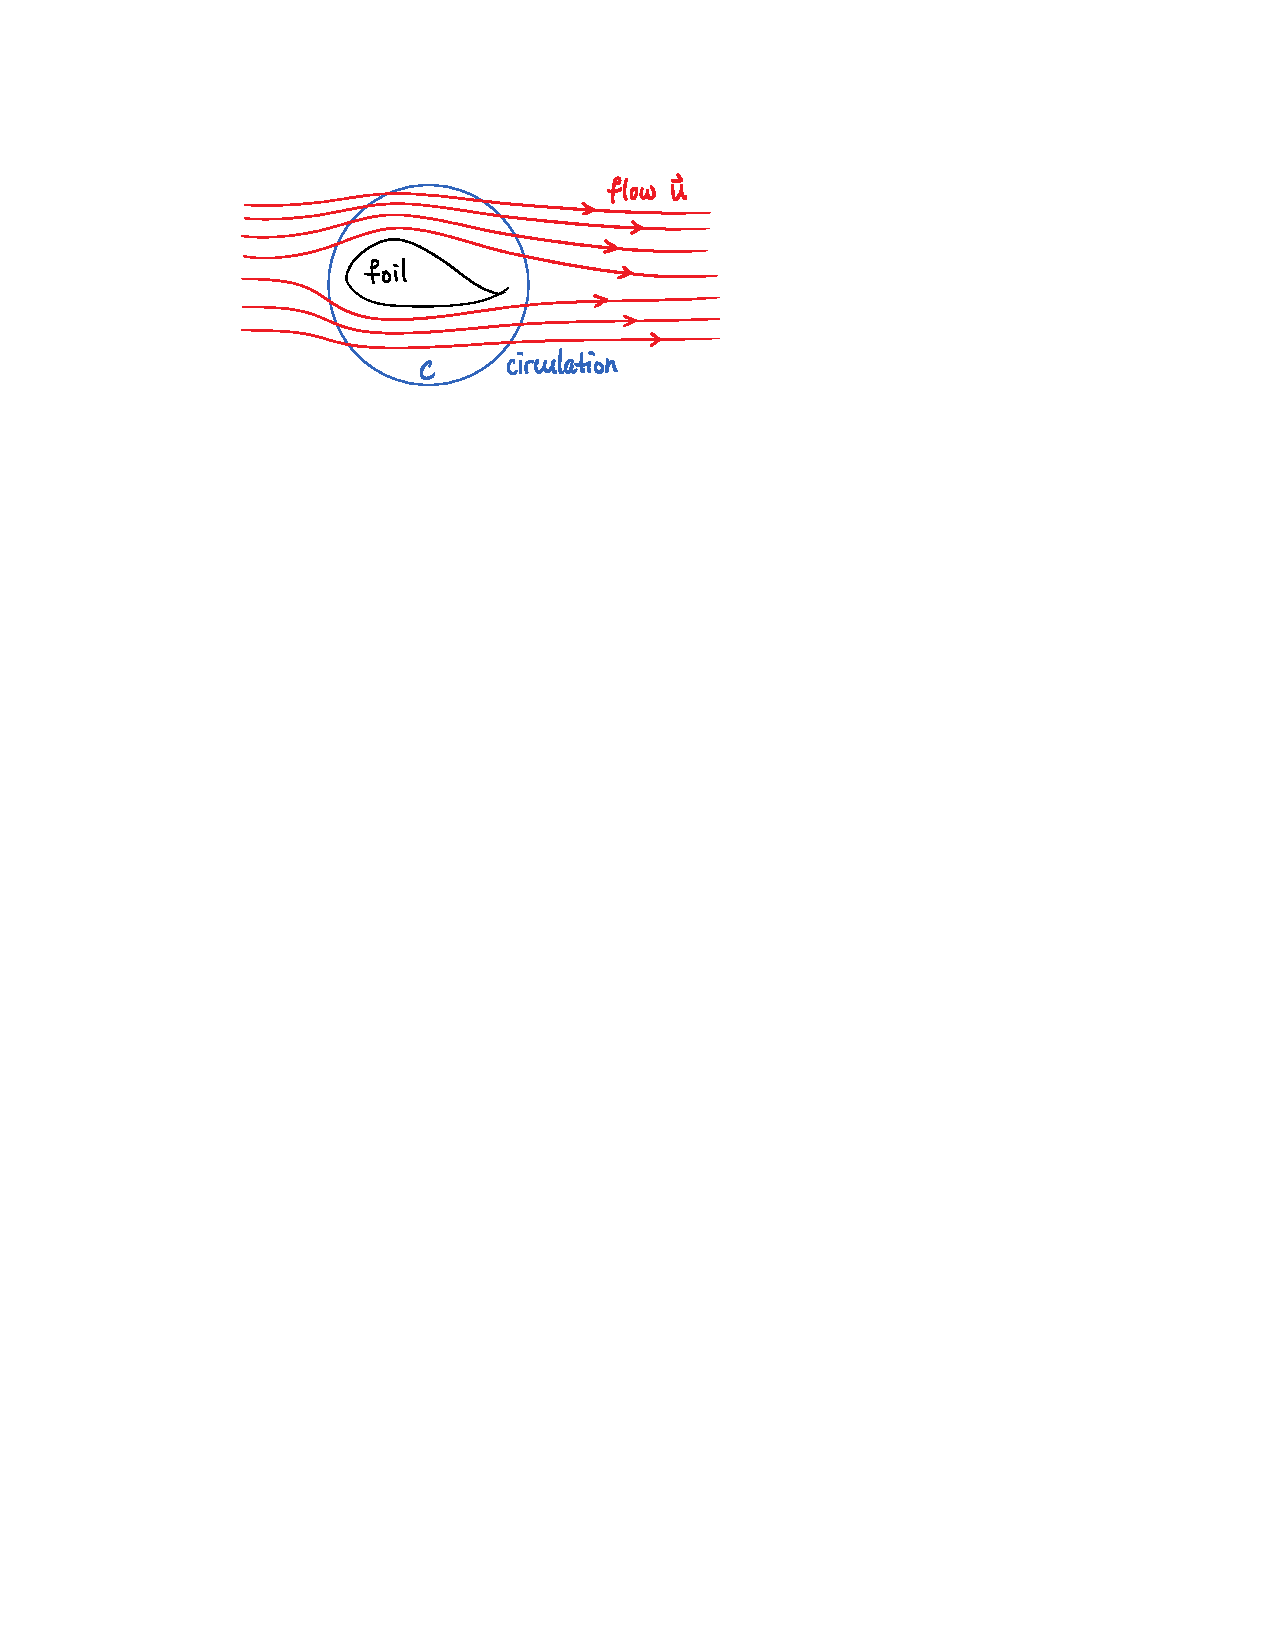
\includegraphics[scale=1.19]{circulation.pdf}
\end{center}


By Stokes Theorem, (1.19) reads the following:
\begin{align*}
\Gamma \coloneqq \int_C \vec{u} \cdot d\vec{x} = \int_A (\nabla \times \vec{u}) \cdot \hat{n}\, dA = \int_A \vec{\omega}\cdot \hat{n} \, dA
\end{align*}
where $A$ is the surface enclosed by the path $C$.\\
In $2$-dimensional flow, (1.19) then reads:
\begin{align*}
\Gamma = \int_A \omega \, dA \tag{2D Flow Circulation}
\end{align*}

\begin{thm}[Kutta-Joukowski Lift Theorem]
The theorem applies to two-dimensional flow around a fixed airfoil. The lift force $F_y$ per unit span of an airfoil with circulation $\Gamma$ is given by:
\begin{align*}
F_y = -\rho\, U_{\infty }\Gamma
\end{align*}
where $\rho$ and $U_{\infty}$ are the fluid density and the fluid velocity far upstream of the airfoil. The circulation $\Gamma$ is calculated by integrating a closed contour enclosing the airfoil and followed in the clockwise direction.
\end{thm}

\newpage
\chapter{Viscous Flow}
\setcounter{section}{4}
\section[Viscosity of a Fluid]{\color{red}Viscosity of a Fluid\color{black}}
\begin{defn}
A stress, or traction, vector $\vec{\tau}$ is a force per unit area on a surface of a fluid. 
\end{defn}

For a stress vector $\vec{\tau}$, we can write:
\begin{align*}
\vec{\tau} = \underbrace{(\vec{\tau}\cdot \hat{n}) \hat{n}}_{\substack{\text{normal stress}\\\text{or the pressure}}} + \ \,  \underbrace{\vec{\tau} - (\vec{\tau} \cdot \hat{n} ) \hat{n}}_{\substack{\text{shear stress}\\ \text{due to viscosity}}}
\end{align*}


\hfill\break
\hfill\break

\example
Suppose the velocity field of a fluid is given by:
\begin{align*}
\vec{u} = (u(y),0,0)
\end{align*}
where $y$ denote the component of the coordinate $\vec{x} = (x,y,z)$. The fluid immediately above some level $y$ exerts a stress on the fluid immediately below and vice versa. The shear stress due to viscosity is given by:
\begin{align}
\tau_{\text{shear}} = \mu \frac{du}{dy}\, \vec{e}_x
\end{align}
where $\mu$ is called the coefficient of viscosity, and $\frac{du}{dy}$ is the shear strain rate. Many real fluids, such as water and air, behave according to (2.1) over a wide range of conditions.\\ 

It is not hard to see from the example above that the dimension of the coefficient of viscosity of the fluid is given by the following:
\begin{align*}
\text{[viscosity]} = \frac{\text{[force]}\cdot \text{[time]}}{\text{[length]}^2} = \frac{\text{[mass]}}{\text{[length]}\cdot \text{[time]}} 
\end{align*}
or one might want to define the kinematic viscosity as:
\begin{align*}
\nu \coloneqq \frac{\mu}{\rho}
\end{align*}
which has dimension given by $\text{[length]}^2 / \text{[time]}$.\\

\begin{center}
\begin{tabular}{|c|c|}
\hline
Material & Kinematic Viscosity\\ 
\hline
water & $0.01\, cm^2/s$\\
\hline
air & $0.15 \, cm^2/s$\\
\hline
glycerin & $18\, cm^2/s$\\
\hline
\end{tabular}
\end{center}

\note For liquid, fluid parcels are attracted to neighboring parcels. \\The viscosity of the liquid decreases as the temperature of the liquid increases.\\


\note For gas, fluid molecules diffuse and collide, so they exchange momentum. \\
The viscosity of the gas increases as the temperature of the gas increases.\\

\remark Flow in the limit of viscosity tending to $0$ is not the same as the fluid with $0$ viscosity. The former is called the singular limit. Observations of viscous fluid flow reveal that both normal and tangential components of fluid velocity at a rigid boundary must be equal to those of the boundary itself. Thus if the boundary is at rest, then $\vec{u} = 0$ there. The condition on the tangential component of velocity is known as the no-slip condition, and it holds for a fluid of any viscosity $\nu \neq 0$, no matter how small $\nu$ is. \\


\newpage
\section[The Navier-Stokes Equations]{\color{red}The Navier-Stokes Equation \color{black}}
For incompressible fluid with zero viscosity, we use the Euler Equations. However, for fluid with nonzero viscosity, the equation of momentum conservation (1.14) fails, for viscous fluid, one needs to write the following for conservation of momentum:
\begin{align}
\frac{\partial \vec{u}}{\partial t} + (\vec{u}\cdot \nabla) \vec{u} = -\frac{1}{\rho}\nabla p + \nu \nabla^2 \vec{u}+ \vec{g}
\end{align}
where for incompressible fluid, we still have (1.11) holds, and hence:
\begin{align}
\nabla \cdot \vec{u} = 0
\end{align}
together, for incompressible fluid, we write the Navier-Stokes equations:
\begin{align}
\frac{\partial \vec{u}}{\partial t} + (\vec{u}\cdot \nabla) \vec{u} = -\frac{1}{\rho}\nabla p + \nu \nabla^2 \vec{u}+ \vec{g} \qquad\qquad\qquad\nabla \cdot \vec{u} = 0
\end{align}
the Navier-Stokes equations is derived in Chapter 6 on Acherson. The term $\nu \nabla^2 \vec{u}$ is called the diffusion of momentum, and $\vec{g}$ is the gravitational field. $(\vec{u}\cdot \nabla) \vec{u}$ is called the inertial term, which has dimension $[\text{velocity}]^2/[\text{length}]$, on the other hand, the viscous term $\nu \nabla^2 \vec{u}$ has dimension $[\nu]\,[\text{velocity}] / [\text{length}]^2$, hence we get:
\begin{align*}
\left[\frac{\text{inertial term}}{\text{viscos term}}\right] = \frac{\text{[length]\, [\text{velocity}]}}{[\nu]}
\end{align*}
and we define:
\begin{align*}
\text{Re} \coloneqq  \frac{L U}{\nu}
\end{align*}
here $\text{Re}$ is called the Reynolds number, and it is estimated using $L$ being the characteristic length scale of the flow, and $U$ being a typical flow speed of the fluid. Note that the choice of $L$ and $U$ are subjective, but should be reasonable for a fluid of interest. The Reynolds number helps predict flow patterns in different fluid flow situations. At low Reynolds numbers, flows tend to be smooth and laminar, while at high Reynolds numbers flows tend to be turbulent. In particular, we observe that $\text{Re}$ has the same order as $(\text{inertial term})/(\text{viscous term})$. \\



\newpage
\example \textbf{Plane parallel shear flow}\\
Consider the plane parallel shear flow defined by the velocity field $\vec{u} = [u(y,t),0,0]$, where $y$ is the $y$-direction position component variable, then the Navier-Stokes equation for such fluid reads the following:
\begin{align*}
\begin{cases}
\frac{\partial u}{\partial t} = -\frac{1}{\rho}\frac{\partial p}{\partial x} + \nu \frac{\partial^2 u}{\partial y^2}\\
\ \ 0 = -\frac{1}{\rho} \frac{\partial p}{\partial y}\\
\ \ 0 = -\frac{1}{\rho} \frac{\partial p}{\partial z} 
\end{cases} \tag{p}
\end{align*}
one can show that we have $p(x,t) = f(t) \cdot x + c(t)$, where $f$ is a function of $t$, and $c(t)$ is a constant at given time $t$. Consider now a block of fluid in such fluid, by Newton's Second Law, we get the following:
\begin{align*}
\rho\, \frac{Du}{Dt}\ \delta x \,\delta y\, \delta z &= (p(x) - p(x+\delta x)) \,\delta y\, \delta z + \mu \left(\left.\frac{\partial u}{\partial y}\right|_{y+ \delta y} - \left.\frac{\partial u}{\partial y}\right|_{y}\right)\,\delta x \, \delta z\\
\rho\ \frac{\partial u}{\partial t} &= \frac{(p(x) - p(x+\delta x))}{\delta x} + \frac{\mu \left( \frac{\partial u}{\partial y}|_{y+ \delta y} - \frac{\partial u}{\partial y}|_{y}\right)}{\delta y}
\end{align*}
which gets us back the system of equation (p). \\

Now consider a no-slip boundary condition for such viscous flow, where the fluid has a solid boundary, hence the boundary condition can be written mathematically by:
\begin{align*}
\vec{u}_{\ \text{fluid at the boundary}} = \text{the velocity of the solid boundary}
\end{align*}
In reality, there is a little slip on molecular scale, the slip length is around $10-50\, nm$ for typical liquid-solid interface, and around $1.15\cdot (\text{mean free path})$ for gas.\\
Consider an impulsively moved boundary, we write:
\begin{align*}
u_{\text{wall}}(t) = \begin{cases} 0 & t< 0 \\ 
U & t \geq 0
\end{cases}
\end{align*}
where $\vec{u}_{\text{wall}}= (u_{\text{wall}}, 0,0)$. Assume that we have $p(\infty,t) = p(-\infty,t)$ where: 
$$p(x,t) = f(t)\cdot x + c(t)$$ 
then we must have $\frac{\partial p}{\partial x} = 0$, hence the first equation in (p) reads:
\begin{align*}
\frac{\partial u}{\partial t} = \nu \frac{\partial^2 u}{\partial y^2} \qquad\qquad\qquad \begin{cases}
u(y,0) = 0 & y>0\\
u(0,t) = U & t\geq 0\\
u(\infty, t) = 0 & t\geq 0
\end{cases} \tag{q}
\end{align*}
which gives a $1$-dimensional heat equation. Here we see that $u$ is a function of $y,t,\nu,U$. In particular, we observe that $u/U$ is a dimensionless function of $y/Ut$, $y/\sqrt{\nu t}$, or any other term that is dimensionless, such that the dimension can match, so we can define:
\begin{align*}
\that{u} \coloneqq \frac{u}{U} \qquad\qquad \that{y} \coloneqq \frac{y}{Ut} \qquad\qquad \eta \coloneqq \frac{y}{\sqrt{\nu t}} \qquad\qquad \cdots
\end{align*}
and hence by argument above, we can write:
\begin{align*}
\that{u} = f(\that{y}, \eta, \cdots)
\end{align*}
To solve (q), we seek a similarity solution. We observe that (q) is unchanged by the transformation of variables $y \mapsto \alpha y$, $t\mapsto \alpha^2 t$, where $\alpha$ is a constant. This suggests the possibility that there are solution to (q) which are functions of $y$ and $t$ simply through the single combination $y/t^{1/2}$, that is, we write $u = f(y/t^{1/2})$. More precisely, we can assume that we have $u = f(\eta)$ where $\eta = y/(\nu t)^{1/2}$, then we can write:
\begin{align*}
\frac{\partial u}{\partial t} = \frac{df}{d\eta} \cdot \frac{\partial \eta}{\partial t} =- f' \frac{y}{\nu^{1/2}}\left(\frac{1}{2} t^{-3/2}\right)
\end{align*}
\begin{align*}
\frac{\partial^2 u}{\partial y^2} = \frac{df}{d\eta}\cdot \frac{\partial^2 \eta}{\partial y^2} + \frac{d^2 f}{d\eta^2} \left( \frac{\partial \eta}{\partial y}\right)^2 = f'' \cdot \frac{1}{\nu t} 
\end{align*}
hence combining via (q) we can get:
\begin{align*}
-\frac{1}{2}f' y \nu^{-1/2}t^{-3/2} =\frac{\nu }{\nu t} f'' \qquad \Rightarrow \qquad -\frac{1}{2}f' \frac{y}{(\nu t)^{1/2}} = f''
\end{align*}
note that $\eta = y/(\nu t)^2$ we have:
\begin{align*}
\frac{\eta}{2}f' + f'' = 0 \qquad \Rightarrow \qquad (f' e^{\eta^2/4})' = 0\qquad \Rightarrow \qquad f'e^{\eta^2/4} = \text{constant}
\end{align*}
so we write:
\begin{align*}
f = A+ B \int_0^\eta e^{-s^2/4}\, ds\qquad\qquad \text{for some }A,B \in \R
\end{align*}
Now we apply the boundary conditions, $f(0) = U$, $f(\infty) = 0$, we get:
\begin{align*}
u(\eta) = f(\eta) = U\left( 1 - \frac{1}{\sqrt{\pi}} \int_0^\eta e^{-s^2/4}\, ds\right) \tag{e}
\end{align*}
the similarity solution states that other form of solution is given by $\frac{u}{U} = g\left(\eta\right)$. Plotting (e) shows that $u$ is significant in the region where $\eta$ has an order of $1$, hence $y$ would have an order of $\sqrt{\nu t}$ when $u$ is significant, such length of $y$ is called the diffusion length. The voracity of such flow is given by the following:
\begin{align*}
\omega = \frac{\partial v}{\partial x} - \frac{\partial u}{\partial y} = \frac{U}{\sqrt{\pi \nu t}}e^{-y^2 / (4\nu t)} \tag{w}
\end{align*}
Note that (e) is also known as the fundamental solution to the $1$-dimensional wave equation. While we see that $\omega$ is also a solution to the $1$-dimensional heat equation of the form given by (q) as we can write the following from equation (w):
\begin{align*}
\frac{\partial \omega}{\partial t} = \nu\frac{\partial^2 \omega}{\partial y^2}
\end{align*}


\newpage
\example \textbf{Steady flow down a flat inclined plane}\\
Consider a flat inclined plane,  we set up a coordinate system such that the $y$-axis is normal to the surface of the incline, and $x$-axis is parallel to the surface of the incline. 
\begin{center}
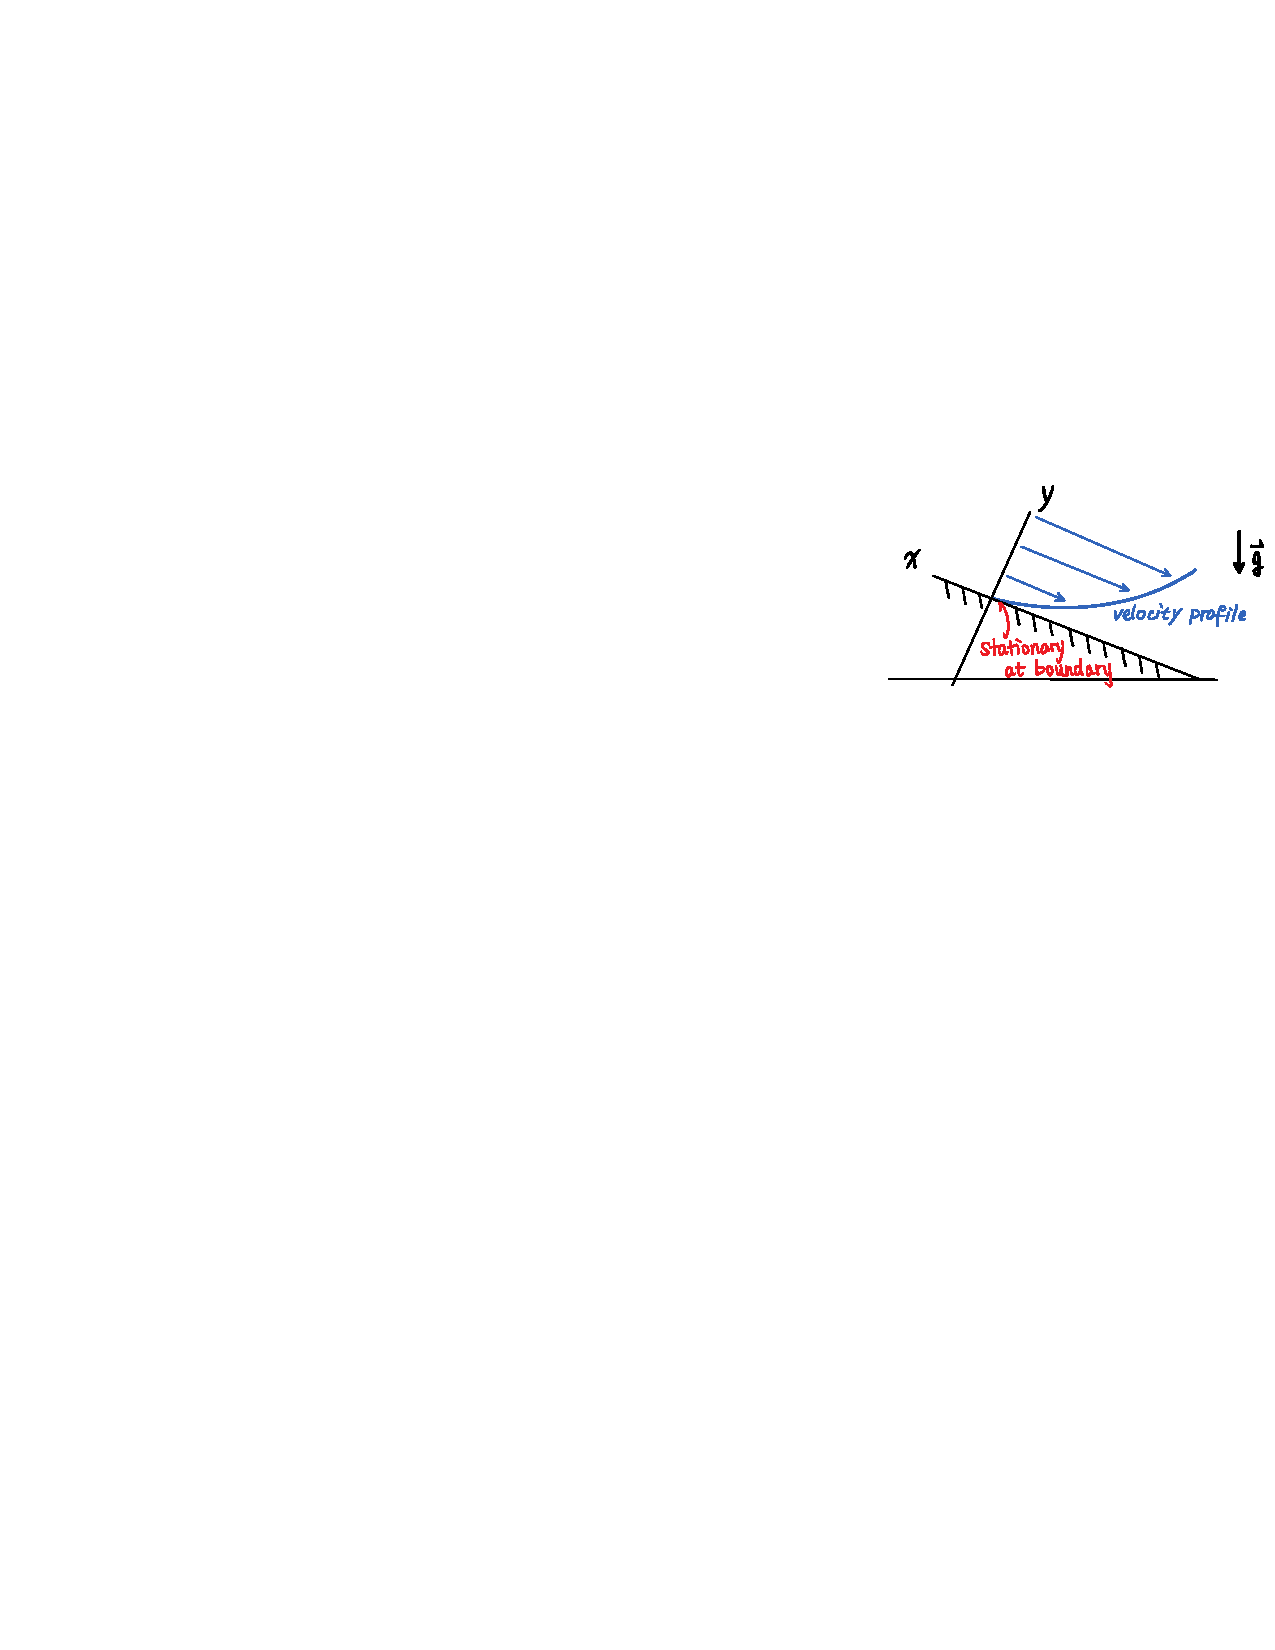
\includegraphics[scale=1.19]{incline.pdf}
\end{center}


Assume that the flow is steady, denoting $\vec{u}=(u,v)$, by incompressibility we can write:
\begin{align*}
\nabla \cdot \vec{u} = \frac{\partial u}{\partial x} + \frac{\partial v}{\partial y}= 0 \tag{s}
\end{align*}
Here for simplicity of the problem, we assume $\frac{\partial u}{\partial x} = 0$, so $u$ is a function of $y$ only. By (s), we see that $v$ must be constant at given $t$, and we have $v(x,0)=0$ by the no-slip condition, then we can conclude that $v = 0$. Now we obtain momentum equation in the Navier-Stokes equations for this system:
\begin{align*}
\frac{\partial u}{\partial t} + (\vec{u} \cdot \nabla) u &= -\frac{1}{\rho} \frac{\partial p}{\partial x} + \nu\frac{\partial^2 u}{\partial y^2} + g\sin(\alpha) \tag{s1}\\
\frac{\partial v}{\partial t} + (\vec{u} \cdot \nabla) v &= -\frac{1}{\rho} \frac{\partial p}{\partial y}  + g\cos(\alpha) \tag{s2}
\end{align*}
where $g$ represents the gravity, and $\alpha$ is the angle between the horizontal and the $x$-axis of the problem. In the problem, we impose stress boundary condition on the top surface, which is considered to be a free surface, and hence implies zero stress on the top surface. At the top of the fluid surface $y = h$: (1) the normal stress component is given by $p(h) = p_0$ where $p_0$ is the atmospheric pressure, and (2) the tangential stress is given by $\mu \frac{du}{dy}|_{y=h} = 0$. At the bottom surface $y=0$, (3) we have the no-slip condition, hence $u = v = 0$. Now using boundary condition (1) applied on (s2), we get the following:
\begin{align*}
p = p_0 + \rho g(h-y)\cos(\alpha)
\end{align*}
and through (2) and (3) applied on (s1), we can write:
\begin{align*}
u = \frac{g}{2\nu} y(2h-y)\sin(\alpha)
\end{align*}
where $h$ is usually set by a volume flux condition. Notice that, experimentally speaking, the fluid is unstable when $\text{Re} \geq 20$, that is, when the Reynolds number of the fluid is large, a small perturbation on the top surface of the fluid, then the perturbation will grow, because the perturbation on the top surface of the fluid distorts all the assumptions that we have applied on the solution, such as steady flow and $\vec{u}$ being independent on $x$. Note that the Reynolds number for such flow is calculated as the following:
$$\text{Re}= \frac{4h\langle u\rangle}{\nu}$$


\newpage
\example 
\textbf{Flow between two walls, one at rest, one started moving impulsively}\\
Consider a layer of fluid between two walls, one on top and one at the bottom. The distance between two walls is fixed by $h$, and the bottom wall starts moving at constant speed $U$ at $t\geq 0$. As example above, we also have:
\begin{align*}
\frac{\partial u}{\partial t} = \nu \frac{\partial^2 u}{\partial y^2}
\end{align*}
and in such case we can write:
\begin{align*}
\frac{u}{U} = f\left(\frac{\nu t}{h^2}, \frac{y}{h}, \cdots \right) \qquad \qquad \begin{cases}
u(0,t) = U & t\geq 0 \\
u(h,t) = 0 & t\geq 0 \\
u(y,0) = 0 & \forall y
\end{cases}
\end{align*}
First, we subtract off a steady solution given by the following:
\begin{align*}
u_s = U\left( 1 - \frac{y}{h}\right)
\end{align*}
then we can write:
\begin{align*} 
u = u_s+u_1 \qquad\qquad\qquad
\begin{cases}
u_1(0,t) = 0 \\ 
u_1(h,t) = 0\\
u_1(y,0) = -u_s(y)
\end{cases}
\end{align*}
Now we employ the method of separation of variables for solving PDE, let $u_1 = Y(y) T(t)$, where $Y$ is a function of a single variable $y$, and $T$ is a function of a single variable $t$. Then the following holds:
\begin{align*}
\frac{YT'}{YT} = \frac{\nu TY''}{TY} = \text{constant}
\end{align*}
because $T'/T$ is a function of $t$ only, and $\nu Y''/Y$ is a function of $y$ only. Now we have $\nu Y '' = (\text{constant})\cdot Y$, where $Y(0) = Y(h) = 0$. Examining the following:
\begin{align*}
Y_n(y) = \sin\left( \frac{n\pi y}{h}\right) \qquad\qquad\qquad\forall n \in \N
\end{align*}
which gives a set of solutions to $Y$, and hence we can solve for $T = T_n$ in the form:
\begin{align*}
T_n(t) = e^{-\frac{n^2 \pi^2}{h^2}\nu t}
\end{align*}
and combining via Principle of Superposition, we get the general form of the solution of $u_1=\sum_n A_n T_n Y_n$ with $A_n \in \R$. Here we write:
\begin{align*}
u_1 = \sum_{n=1}^\infty A_n e^{-\frac{n^2 \pi^2}{h^2}\nu t} \sin\left( \frac{n \pi y}{h}\right)
\end{align*}
where $A_n$ can be computed using the initial conditions. Finally, we get:
\begin{align*}
u = u_s + u_1 =U\left(1-\frac{y}{h}\right)+ \sum_{n=1}^\infty A_n e^{-\frac{n^2 \pi^2}{h^2}\nu t} \sin\left( \frac{n \pi y}{h}\right) 
\end{align*}

\newpage
\example \textbf{Circular flow}\\
The velocity field of the circular flow is characterized by:
\begin{align*}
\vec{u} = u_{\theta} (r,t) \vec{e}_{\theta}
\end{align*}
and we can write $\vec{u} = (u_{r}, u_{\theta}, u_z)$, with $u_r = u_z = 0$. \\
By Navier-Stokes equations, we can write the following:
\begin{align}
\begin{cases}
\frac{u_{\theta}^2}{r} = \frac{1}{\rho} \frac{\partial p}{\partial r}\\
\frac{\partial u_{\theta}}{\partial t} = -\frac{1}{\rho r}\frac{\partial p}{\partial \theta} + \nu\left(\frac{\partial^2 u_{\theta}}{\partial r^2} + \frac{1}{r}\frac{\partial u_{\theta}}{\partial r} - \frac{u_{\theta}}{r^2}\right)\\
0 = \frac{1}{\rho} \frac{\partial p}{\partial z}
\end{cases} \tag{c}
\end{align}
and the incompressibility equation in cylindrical coordinate:
\begin{align*}
\nabla \cdot \vec{u} = \frac{1}{r} \frac{\partial (ru_r)}{\partial r} + \frac{1}{r}\frac{\partial u_{\theta}}{\partial \theta}+ \frac{\partial u_z}{\partial z} = 0
\end{align*}
From the second line of (c), we get the following:
\begin{align*}
\frac{\partial p}{\partial \theta} = g(r,t) \qquad \Rightarrow \qquad p = g(r,t) \cdot \theta + f(r,t)
\end{align*}
but pressure is continuous, hence $g(r,t) \cdot \theta$ must be dropped as $p$ is continuous at $\theta = 0$ and $\theta = 2\pi$. That is, now we can write the following:
\begin{align*}
p = f(r,t) \qquad\qquad\qquad \frac{\partial p}{\partial \theta} = 0
\end{align*}
Now consider the circular steady flow between rotating walls, and by second equation in (c) applied with argument above, we can write:
\begin{align*}
0 = \frac{\partial u_{\theta}}{\partial t} = \nu\left(\frac{\partial^2 u_{\theta}}{\partial r^2} + \frac{1}{r}\frac{\partial u_{\theta}}{\partial r} - \frac{u_{\theta}}{r^2}\right) \tag{t}
\end{align*}
solving (t) we get the following form of $u_{\theta}$:
\begin{align*}
u_{\theta} = Ar + \frac{B}{r}
\end{align*}
where $A,B$ are determined by boundary conditions.\\

Now consider the circular flow is spun up in a cylinder, in such case we are in a unsteady problem. Suppose the outer boundary at radius $a$ spins at angular velocity $\Omega_0$ when $t\geq 0$, then here we write the following boundary conditions:
\begin{align*}
u_{\theta}(a,t) = \begin{cases}
0 & t< 0 \\
\Omega_0 a & t\geq 0
\end{cases}
\end{align*}
In such case the solution of the problem is given by the following:
\begin{align*}
u_{\theta}(r,t) = \Omega_0 t + 2\Omega_0 a \sum_{n=1}^\infty \frac{J_1(\lambda_n r/a)}{\lambda_n J_0(\lambda_n)}\cdot e^{-\frac{\lambda_n^2 \nu t}{n^2}}
\end{align*}

\newpage
\chapter{Fluid Waves}
\setcounter{section}{6}
Consider a $2$-dimensional water wave, whose velocity field is characterized by:
\begin{align*}
\vec{u} = [u(x,y,t),\ v(x,y,t),\ 0]
\end{align*}
with the top surface defined by a function $y = \eta(x,t)$, and the top surface is characterized by a free surface interface condition $p = p_0$, where $p_0$ represents the air pressure. 

\section[Deep Water Waves]{\color{red} Deep Water Waves \color{black}}
Assume that there is no bottom surface, that is $y$ can approach to $-\infty$ and $\vec{u}$ is still well defined, and assume that $\omega = 0$ for such flow, that is the flow is irrotational. Note that in $2$-dimensional inviscid flow,, one can obtain $\frac{D\omega}{Dt}= 0$, that is, if $w = 0$ initially, then $w = 0$ for all $t$. \\

For such $2$-dimensional flow, let $o,p$ be points in the flow, and let $C_1$ be a path connecting the two points, one can define a velocity potential $\phi$ at $p$ by the following:
\begin{align*}
\phi \coloneqq \int_0^p \vec{u}\cdot d\vec{x} \coloneqq \int_{C_1} \vec{u}\cdot d\vec{x}
\end{align*}
Note that $\phi$ is path-independent for irrotational flow in a simply connected domain, that is, for paths $C_1, C_2$ connecting $o$ and $p$, according to Green's Theorem, with $\omega = \nabla\times \vec{u} = 0$, we have the following holds:
\begin{align*}
\int_{C_1} \vec{u}\cdot d\vec{x} - \int_{C_2} \vec{u}\cdot d\vec{x} = \int_A \omega \, dA = 0
\end{align*}
where $A$ is the area enclosed by the two paths $C_1$ and $C_2$. Moreover, we can write:
\begin{align*}
\phi = \int_o^p u\, dx + v \, dy \qquad \Rightarrow \qquad \frac{\partial \phi}{\partial x} = u\qquad\qquad \frac{\partial \phi}{\partial y} = v
\end{align*}
that is, we write: 
\begin{align*}
\nabla \phi = \vec{u}
\end{align*}
If one assumes the incompressible fluid condition $\nabla \cdot \vec{u} = 0$, then it follows that $\nabla^2 \phi = 0$. \\

For boundary conditions of a flow, one can have two types of boundary conditions, the first type is the kinematic condition, that is, on the boundary surface, we have the fluid velocity component normal to boundary surface being equal to the interface velocity component normal to the boundary surface. Mathematically, at a point on the boundary surface $(x(\alpha,t), y(\alpha,t))$, by choosing $\alpha = x$, the tangential vector is given by:
\begin{align*}
\hat{s} = \frac{\left( \frac{\partial x}{\partial \alpha}, \frac{\partial y}{\partial \alpha}\right)}{\sqrt{\left( \frac{\partial x}{\partial \alpha}\right)^2 + \left( \frac{\partial y}{\partial \alpha}\right)^2 }} = \frac{\left( 1, \frac{\partial \eta}{\partial x}\right)}{\sqrt{1+\left( \frac{\partial \eta}{\partial x}\right)^2 }}
\end{align*}
and the normal vector is given by:
\begin{align*}
\hat{n} = \frac{\left( -\frac{\partial \eta}{\partial x}, 1 \right)}{\sqrt{1+ \left( \frac{\partial \eta}{\partial x}\right)^2}}
\end{align*}
and the kinematic boundary condition reads:
\begin{align*}
\bmat{u\\ v}\cdot \hat{n} = \bmat{0 \\ \frac{\partial \eta}{\partial t}}\cdot \hat{n}
\qquad\quad\Rightarrow\qquad\quad
-u \, \frac{\partial \eta}{\partial x} + v = \frac{\partial \eta}{ \partial t} \tag{K}
\end{align*}

The second type of boundary conditions is given by the Bernoulli's Theorem. For irrotational flow, through the Bernoulli's equation for unsteady flow, we can write:
\begin{align*}
\frac{\partial }{\partial t}\left( \nabla \phi\right) =  \frac{\partial \vec{u}}{\partial t} = -\nabla \left( \frac{p}{\rho} + \frac{1}{2}||\vec{u}||^2 + \chi\right)
\end{align*}
where $\chi = gy$, that is, we have:
\begin{align*}
\nabla \left( \frac{\partial \phi}{\partial t} + \frac{p}{\rho} + \frac{1}{2}||\vec{u}||^2 + \chi\right)= 0
\end{align*}
and hence we can write:
\begin{align}
\frac{\partial \phi}{\partial t} + \frac{p}{\rho} + \frac{1}{2}||\vec{u}||^2 + \chi = G(t) 
\end{align}
where $G(t)$ is an arbitrary function that can be absorbed into $\phi$ without changing $\nabla \phi$. 
At the free surface, $p = p_0$, and $y = \eta(x,t)$, then can set $G(t) = p_0 / \rho$, in which case (3.1) becomes the following:
\begin{align*}
\frac{\partial \phi}{\partial t} + \frac{1}{2}\left(u^2 + v^2\right) + g\eta = 0 \tag{B}
\end{align*}
Now equation (K) and equation (B) characterize the two boundary conditions in our example problem. 
Now we focus on small-amplitude solutions, where we assume $|\eta| \ll 1$ and $|u|,|v|,|\phi| \ll 1$. Hence we can eliminate the quadratic terms in the boundary conditions, now the two boundary conditions (K) and (B) now reads:
\begin{align*}
\frac{\partial \phi}{\partial y}  = \frac{\partial \eta}{\partial t} \qquad&\text{ at } y = \eta(x,t) \approx 0 \tag{K1}\\ 
\frac{\partial \phi}{\partial t} + g\eta = 0\qquad&\text{ at } y = \eta(x,t) \approx 0  \tag{B1}
\end{align*}
Note that, in the region of interest $y \leq \eta(x,t) \approx 0$, we want a solution to $\phi$ that satisfies the Laplace's equation of the form given by the following: 
\begin{align*}
\nabla^2 \phi = 0
\end{align*}
It turns out that there are infinitely many solutions to this problem. Here we try solutions of the form where $\eta$ is given by the following:
\begin{align*}
\eta = Ae^{ikx} e^{iw t} = A\cos(kx - wt)
\end{align*}
Equation (B1) requires:
\begin{align*}
\frac{\partial \phi}{\partial t} = -g A \cos(kx-wt) \qquad\text{at }y=0	 \tag{B2}
\end{align*}
Equation (K1) requires:
\begin{align*}
\frac{\partial \phi}{\partial y} = w A \sin(kx-wt) \qquad \text{at }y=0    \tag{K2}
\end{align*}
Here we try $\phi = f(y) \sin(kx-wt)$. Apply the Laplace equation for $\phi$ we get:
\begin{align*}
\frac{\partial^2 \phi}{\partial x^2} + \frac{\partial^2 \phi}{\partial y^2} = 0 \qquad \Rightarrow \qquad -k^2 f\sin(kx-wt) + f'' \sin(kx-wt) = 0
\end{align*}
so we requires the function $f$ to be the form with $C,D \in \R$ given by the following:
\begin{align*}
f = Ce^{ky} + De^{-ky}
\end{align*}
we must set $D = 0$ such that $v = \frac{\partial \phi}{\partial y}$ is bounded as $y$ approaches $-\infty$. Now we get:
\begin{align*}
\phi = C e^{ky} \sin(kx-wt) \tag{G}
\end{align*}
Here we want $\phi$ to satisfies both (B2) and (K2), hence we write:
\begin{align*}
\left.\frac{\partial \phi}{\partial t}\right|_{y=0} = -w C\cos(kx-wt) = -gA \cos(kx-wt) \qquad \Rightarrow \qquad C = \frac{gA}{w}
\end{align*}
\begin{align*}
\left.\frac{\partial \phi}{\partial y}\right|_{y=0} = kC \sin(kx-wt) = wA \sin(kx-wt) \qquad \Rightarrow \qquad C = \frac{wA}{k}
\end{align*}
In which case we require the following holds:
\begin{align*}
\bmat{g & -w \\ w & k} \bmat{A \\ C} = \bmat{ 0 \\ 0}
\end{align*}
in other words, we must have the parameters satisfying the following:
\begin{align*}
w^2 = gk
\end{align*}
and such condition is called the dispersion relation. Now we get the final solution $\phi$:
\begin{align}
\phi = \frac{Aw}{k}e^{ky}\sin(kx-wt) = \frac{Aw}{k}e^{ky} \sin(k(x-ct))
\end{align}
where $c = w/k$ is the phase speed of the wave associated ot $k$:
\begin{align*}
c = \frac{w}{k} = \frac{\sqrt{gk}}{k} = \sqrt{\frac{g}{k}}
\end{align*}
and here we see that wave with longer wavelength moves faster for our example, the waves characterized by (3.2) are called the gravity waves. Moreover, the particle paths for the flow defined by (3.2) can be computed as $\vec{x}= (x(t),y(t))$ by the following:
\begin{align*}
x(t) &= \bar{x} + \hat{x}(t) \qquad \Rightarrow \qquad \frac{d}{dt}\left( \bar{x} + \hat{x}(t) \right) = u(\bar{x}+ \hat{x}, \bar{y} + \hat{y} , t)\approx u(\bar{x}, \bar{y}, t) \\
y(t) &= \bar{y} + \hat{y}(t) \qquad \Rightarrow \qquad \frac{d}{dt}\left( \bar{y} + \hat{x}(t) \right) = v(\bar{x}+ \hat{x}, \bar{y} + \hat{y} , t)\approx u(\bar{x}, \bar{ y}, t) 
\end{align*}
where $\bar{x},\bar{y} \in \R$ are initial positions of the particle, and we assume that $\hat{x}(t)$ and $\hat{y}(t)$ are small. Now we can write:
\begin{align}
\frac{d}{dt} \hat{x} = Aw e^{k\bar{y}} \cos(k\bar{x} - wt) \qquad &\Rightarrow \qquad \hat{x}(t) = -A e^{k\bar{y}}\sin(k\bar{x}-wt)\\
\frac{d}{dt} \hat{y} = Aw e^{k\bar{y}} \sin(k\bar{x} - wt) \qquad &\Rightarrow \qquad \hat{y}(t) A e^{k\bar{y}}\cos(k\bar{x}-wt)
\end{align}
here (3.3) and (3.4) together describes circular paths of the particles. \\
\hfill\break

\subsection{Motion of the wave packet}
Now take a superposition of surface waves of a gravity wave, let $a(k)$ denote the amplitude of a wave associated to $k = w/c$, and let $w$ be a function of $k$ such that $w^2 = gk$. We can write the following:
\begin{align*}
\eta(x,t) = \int_{-\infty}^\infty a(k) e^{i(kx-w(k)t) }\, dk
\end{align*}
Assume that $|a(k)|$ is large for some $k$ near $k_0$, and such assumption is called the wave packet condition, which characterizes the overall shape of the wave. Then we can apply a Taylor expansion of $w$ about $k$ near $k_0$ and get the following:
\begin{align*}
w(k) = w(k_0) + (k-k_0) \left.\frac{dw}{dk}\right|_{k_0} +( \text{higher order terms})
\end{align*}
here $c_g \coloneqq \frac{dw}{dk}|_{k_0}$ is called the group speed, and for the deep water wave under gravity, the group speed is given by: 
$$c_g = \left.\frac{d(\sqrt{gk})}{dk}\right|_{k_0} = \frac{1}{2}\frac{\sqrt{g}}{\sqrt{k_0}} = \frac{1}{2}\sqrt{\frac{g}{k_0}}$$
compared to the phase speed of the wave associated to $k_0 = w/ c$:
\begin{align*}
c = \frac{w}{k_0} = \frac{\sqrt{gk_0}}{k_0} = \sqrt{\frac{g}{k_0}}
\end{align*} 
we see that for gravity wave, we have $c=2\cdot c_g$. 
Now we can write:
\begin{align*}
\eta(x,t) &\approx \int_{-\infty}^\infty a(k) e^{ik_0x} e^{i(k-k_0)x} e^{-iw(k_0)t} e^{-i(k-k_0)c_g t}\, dk\\
&=\underbrace{\vphantom{\int_{-\infty}^\infty a(k)}e^{i(k_0x-w(k_0)t)}}_{\substack{\text{sinusoidal wave,}\\ \text{wave number }k_0}} \ \ \cdot \ \  \underbrace{ \int_{-\infty}^\infty a(k) e^{i(k-k_0)(x-c_g t)}\, dk}_{\substack{\text{superposition of long wavelengths,}\\ \text{functions of }x-c_gt, \text{ with speed }c_g, \\ \text{forming the envelop of the wave}}}
\end{align*}
Here we can write:
\begin{align*}
f(x-c_g t) \coloneqq \int_{-\infty}^\infty a(k) e^{i(k-k_0)(x-c_g t)}\, dk
\end{align*}
Then we get:
\begin{align*}
\eta(x,t) \approx e^{i(k_0x-w(k_0)t)} \cdot f(x-c_g t)
\end{align*}

\hfill\break

\subsection{Long-time solution}
Here we are trying to describe the wavetrain, a succession of wave patterns on the surface of the fluid occurring at periodic intervals when we observe the wave in a long period of time. We assume that in the long run, the waves are approximately sinusoidal with slowly varying wavenumber $k$, here we assume that we have:
\begin{align*}
\eta(x,t) = A(x,t)\cdot e^{i\,\theta(x,t)}
\end{align*}
where $\theta(x,t)$ is called the phase function. We also assume that $A,\frac{d\theta}{dx}, \frac{d\theta}{dt}$ vary slowly in $x$ and $t$. Then we can write the Taylor expansion of $\theta$ around $(x_0,t_0)$:
\begin{align*}
\theta(x,t) = \theta(x_0 , t_0) + \left.\frac{\partial \theta}{\partial x}\right|_{(x_0,t_0)}(x-x_0) + \left.\frac{\partial \theta}{\partial t}\right|_{x_0,t_0}(t-t_0) + \text{(higher order terms)}
\end{align*}
the higher order terms can be neglected because we have assumed that $d\theta/dx$ and $d\theta/dt$ vary slowly in $x$ and $t$. Being consistent with what we have discussed above, we can define the followings:
\begin{align*}
k &\coloneqq \left.\frac{\partial \theta}{\partial x}\right|_{(x_0,t_0)} = \text{ local wavenumber}\\
-\omega &\coloneqq \left.\frac{\partial \theta}{\partial t}\right|_{(x_0,t_0)} = -\text{ local frequency}
\end{align*}
assume that $\omega(k)$ is known, we can write the following by definition of $k$ and $-\omega$:
\begin{align*}
\frac{\partial k}{\partial t} + \frac{\partial \omega}{\partial x} =\frac{\partial k}{\partial t} + \frac{d \omega}{d k}\cdot \frac{\partial k}{\partial x}  =0
\end{align*}
that is $k$ is conserved if one moves with the wave at the group velocity $c_g = \frac{d\omega}{dk}$. \\

\subsubsection{Application in deep water waves}
Here we want to find $\theta(x,t)$, where we have $\omega = \sqrt{gk}$, and $c_g(k) = (1/2)\sqrt{g/k}$. Suppose we observe a wave with wavenumber $k$ at $(x,t) = (0,0)$. If we move with the wave at speed $c_g(k)$, that is $x = c_g(k) \cdot t = (1/2) \sqrt{g/k} \, t$, we still see wavenumber $k$, and here we require:
\begin{align*}
x = c_g(k) \cdot t = (1/2) \sqrt{g/k} \, t \qquad \Rightarrow \qquad k =\frac{gt^2}{4x^2} \qquad \omega = \sqrt{gk}=\frac{gt}{2x}
\end{align*}
Hence we get:
\begin{align*}
\frac{\partial \theta}{\partial x} = k = \frac{gt^2}{4x^2} \qquad\qquad\qquad -\frac{\partial \theta}{\partial t} = \frac{gt}{2x} 
\end{align*}
and combining we get:
\begin{align*}
\theta(x,t) = -\frac{gt^2}{4x}+\epsilon
\end{align*}
that is the surface is characterized by:
\begin{align}
\eta(x,t) = A(x,t)\cdot e^{-i \cdot \frac{gt^2}{4x}}
\end{align}
Notice that we also have:
\begin{align*}
\lambda = \frac{2\pi}{k} \propto \frac{x^2}{gt^2} \qquad \Rightarrow \qquad \frac{\Delta \lambda}{\Delta x} \approx \frac{\partial \lambda}{\partial x} \propto \frac{x}{gt^2}
\end{align*}
Let $\Delta x = \lambda$, we argue that if $\Delta x/\lambda <<1 $, the wave will look approximately sinusoidal, that is, we want the following holds in order to see an approximately sinusoidal wave:
\begin{align}
\frac{\Delta \lambda}{\lambda} \propto \frac{x}{gt^2} << 1 
\end{align}
Here we conclude that $\eta$ is approximately sinusoidal when (3.6) holds. \\

\hfill\break
\subsection{Capillary waves}
Consider a small parcel of fluid at the horizontal region $(x, x+\delta x)$ at the surface of the flow, and suppose the surface of the flow is not perfectly flat, nor greatly deformed, the vertical component of the surface tension of the parcel is given by the following:
\begin{align*}
-T \left.\frac{\partial \eta}{\partial x}\right|_x + T \left.\frac{\partial \eta}{\partial x}\right|_{x+\delta x}
\end{align*}
which is equal to the negative vertical component of the pressure force at the region $(x,x+\delta x)$, denoted as $(p_0 - p)\cdot \delta x$. Taking $\delta x$ to be small enough we can write:
\begin{align*}
T \, \frac{\partial^2 \eta}{\partial x^2} = p_0 - p
\end{align*}
The Bernoulli's Theorem stated as (3.1) reads the following:
\begin{align*}
\frac{\partial \phi}{\partial t} + \frac{p}{\rho} + \frac{1}{2}||\vec{u}||^2 + g\eta = G(t)
\end{align*}
and here we can set $G(t) = p_0 / \rho$. At $y = \eta(x,t)$ we get:
\begin{align*}
\frac{\partial \phi}{\partial t} +\frac{(p-p_0)}{\rho} + \frac{1}{2}||\vec{u}||^2 + g\eta = 0
\end{align*}
we linearize the equation by assuming that $y = \eta(x,t) \approx 0$, hence $(1/2)||\vec{u}||^2 \approx 0$. Now we get the following PDE for $\phi$:
\begin{align}
\frac{\partial \phi}{\partial t} + g\eta - \frac{T}{\rho}\frac{\partial^2 \eta}{\partial x^2} = 0
\end{align}
The assumption of setting $\eta = A\cos(kx-\omega t)$ can still give us a solution to (3.7), with solution satisfying the followings:
\begin{align*}
\omega^2 = gk+\frac{Tk^3}{\rho} \qquad\qquad\qquad c=\frac{\omega}{k} = \left( \frac{gk}{k^2} + \frac{Tk^3}{\rho k^2}\right)^{1/2} = \left( \frac{g}{k}+ \frac{Tk}{\rho}\right)^{1/2}
\end{align*}
If the surface tension term $Tk^2/\rho$ is approximately equal to the gravity term $g$, we write:
\begin{align*}
g \approx \frac{Tk^2}{\rho } \qquad \Rightarrow \qquad \lambda = \frac{2\pi }{k} \approx 1.7\, cm \text{ for water waves}
\end{align*}
If the surface tension is much larger than gravity, we get capillary waves, in which case the phase speed for the wave is given by the following:
\begin{align*}
c_{cap} \approx \left( \frac{Tk}{\rho}\right)^{1/2}
\end{align*}
that is, we see that the phase speed is larger for larger wavenumber $k$. \\
The group speed for capillary waves is given by the following:
\begin{align*}
c_{g,cap} = \frac{d\omega}{dk} = \frac{d}{dk}\left( \sqrt{\frac{T}{\rho}}\, k^{3/2}\right) = \frac{3}{2}\sqrt{\frac{Tk}{\rho}} = \frac{3}{2}\, c_{cap}
\end{align*}
hence, for capillary waves, the group speed is faster than the individual phase wave speed.\\

On the other hand, if the gravity is much larger than the surface tension, then we get gravity waves, whose phase speed is given by:
\begin{align*}
c_{grav} \approx \left( \frac{g}{k}\right)^{1/2}
\end{align*}
and the group speed for gravity wave is given by the following:
\begin{align*}
c_{g, grav} = \frac{d}{dk}\left( \sqrt{gk}\right) = \frac{1}{2}\sqrt{\frac{g}{k}} = \frac{1}{2}\, c_{grav}
\end{align*}


\subsection{Finite depth water waves}
In section 3.1.1, we derived a general solution for velocity potential of the flow of deep water wave given by equation (G), before applying the boundary conditions for deep water, (G) reads the following:
\begin{align*}
\phi(x,y,t) = (Ce^{ky} + De^{-ky})\sin(kx-\omega t) \tag{G}
\end{align*}
In section 3.1.1, we applied the deep water wave boundary conditions to (G) to determine $C$ and $D$. Now, instead, we assume the boundary conditions of finite depth water wave to be the kinematic condition given by (K2), Bernoulli's condition given by (B2), and the condition that there is no penetration at the bottom surface at finite depth $-h$:
\begin{align*}
\left.\frac{\partial \phi}{\partial y}\right|_{y=-h} = 0
\end{align*}
solving for $C$ and $D$, we get:
\begin{align*}
\omega^2 = gk \tanh(kh)\qquad\qquad\qquad c^2=\frac{g}{k}\tanh(kh)
\end{align*}
For shallow water, $kh<<1$, and hence $\tanh(kh)\approx kh$, in which case we have $c^2 \approx gh$, getting the nondispersive waves. \\


\hfill\break
\subsection{Sound Waves}
In this setting, we employ the momentum equation while neglecting the viscosity:
\begin{align}
\rho\left( \frac{\partial \vec{u}}{\partial t} + (\vec{u}\cdot \nabla )\vec{u}\right) = -\nabla \rho
\end{align}
we also employ the mass conservation equation:
\begin{align}
\frac{\partial \rho}{\partial t} + \nabla \cdot (\rho \vec{u}) = 0
\end{align}
and we also want to apply the equation of state for an ideal gas:
\begin{align*}
\frac{D}{Dt}(p \rho^{-\gamma}) = 0 \qquad\qquad \gamma = \frac{c_p}{c_V}\qquad\quad c_p = \left( \frac{\delta Q}{\delta T}\right)_{\delta p=0} \qquad\quad c_V = \left( \frac{\delta Q}{\delta T}\right)_{\delta V = 0}
\end{align*}
The rest state of the gas is assumed to be the following:
\begin{align*}
\vec{u} = \vec{u}_0 = \vec{0} \qquad\qquad p=p_0 \qquad\qquad \rho = \rho_0
\end{align*}
Here we linearize our problem for small change from the rest state:
\begin{align*}
\vec{u} = \vec{u}_0 + \vec{u}_1 = \vec{u}_1\qquad\qquad p = p_0+p_1 \qquad\qquad \rho = \rho_0 + \rho_1
\end{align*}
The equation of state of the ideal gas now reads:
\begin{align*}
p\rho^{-\gamma} = p_0 \rho_0^{-\gamma} = (p_0+p_1)(\rho_0+\rho_1)^{-\gamma}
\end{align*}
rearranging and dropping higher order terms, we get:
\begin{align*}
p_0 \rho_0^{-\gamma}\left(1+\frac{p_1}{p_0}\right)\left( 1+ \frac{\rho_1}{\rho_0}\right)^{-\gamma} &= p_0\rho_0^{-\gamma}\\
\left(1+\frac{p_1}{p_0}\right)\left( 1+ \frac{\rho_1}{\rho_0}\right)^{-\gamma} &= 1\\
\left(1+ \frac{\rho_1}{\rho_0} \right)\left( 1- \gamma \frac{\rho_1}{\rho_0}+\cdots\right)&= 1\\
1+ \frac{p_1}{p_0} - \gamma \frac{\rho_1}{\rho_0}+\cdots &= 1
\end{align*}
hence approximately we have:
\begin{align}
p_1 = \gamma \frac{p_0}{\rho_0}\rho_1
\end{align}
where we can define:
\begin{align}
a_0^2 \coloneqq \gamma \frac{p_0}{\rho_0}
\end{align}
Now we also linearize the momentum equation (3.8) and the mass conservation equation (3.9) for this problem and get the followings:
\begin{align}
\rho_0 \frac{\partial \vec{u}_1}{\partial t} = -\nabla p_1 \qquad\qquad\qquad  \frac{\partial \rho_1}{\partial t} + \rho_0 \nabla \cdot \vec{u}_1 = 0
\end{align}
combining (3.10), (3.11), and (3.12), we have:
\begin{align}
\frac{\partial^2 \rho_1}{\partial t^2} = \nabla^2 p_1 = a_0^2 \nabla^2 \rho_1
\end{align}
For $1$-dimensional, (3.13) reads:
\begin{align*}
\frac{\partial^2 \rho_1}{\partial t^2} = a_0^2 \frac{\partial \rho_1^2}{\partial x^2}
\end{align*}
solving we get:
\begin{align*}
\rho_1 = f(x-a_0 t) + g(x+a_0 t)
\end{align*}
for some function $f$ and $g$, describing waves traveling in opposite directions. \\

\subsection{Steady compressible flow past an airfoil}
Consider the base flow that solves the Navier-Stokes equations: 
\begin{align*}
\vec{u} =(u,v)= U \vec{e}_x \qquad\qquad p=p_0 \qquad\qquad\rho = \rho_0
\end{align*}
Here we apply a little perturbation to the flow:
\begin{align*}
\vec{u} = (U+u_1) \vec{e}_x+v_1\vec{e}_y \qquad\qquad p=p_0+p_1 \qquad\qquad\rho = \rho_0+\rho_1
\end{align*}
We seek for a steady solution, that is $\vec{u}$ is independent of $t$.\\
Here the state equation for ideal gas reads:
\begin{align}
\frac{D}{Dt}( p \rho^{-\gamma}) = 0 \qquad\Rightarrow\qquad p_1 = a_0^2\rho_1
\end{align}
the momentum equation, neglecting viscosity, reads:
\begin{align*}
\rho((\vec{u}\cdot \nabla)\vec{u}) = -\nabla p \qquad \Rightarrow \qquad (\rho_0+\rho_1) \left( (U+u_1)\frac{\partial u_1}{\partial x} + v_1 \frac{\partial u_1}{\partial y}\right) = -\frac{\partial p_1}{\partial x}
\end{align*}
where we can linearize the terms again and get:
\begin{align}
\rho_0 \, U \frac{\partial u_1}{\partial x} = -\frac{\partial p_1}{\partial x} \qquad\qquad \rho_0\, U\frac{\partial v_1}{\partial x} = -\frac{\partial p_1}{\partial y}
\end{align}
combining we have:
\begin{align*}
\rho_0\, U \frac{\partial }{\partial x}\left( \frac{\partial u_1}{\partial y} - \frac{\partial v_1}{\partial x}\right) = 0
\end{align*}
where we set:
\begin{align*}
u_1 = \frac{\partial \phi}{\partial x}\qquad\qquad\qquad v_1 = \frac{\partial \phi}{\partial y}
\end{align*}
and hence from (3.15) we can write:
\begin{align*}
-\frac{\partial p_1}{\partial x} = \rho_0 U \frac{\partial^2 \phi}{\partial x^2}
\qquad\Rightarrow\qquad
p_1 = -\rho_0 U \frac{\partial \phi}{\partial x}+\text{constant}
\end{align*}
we drop the constant and write:
\begin{align}
p_1 = -\rho_0 U \frac{\partial \phi}{\partial x}
\end{align}

For the mass conservation equation, assuming steady flow, we get:
\begin{align*}
\nabla\cdot (\rho \vec{u}) = 0 \qquad \Rightarrow \qquad \rho (\nabla \cdot \vec{u})+ \vec{u}\cdot \nabla \rho = 0
\end{align*}
dropping the nonlinear terms, we have:
\begin{align*}
\rho\left(\frac{\partial u_1}{\partial x} + \frac{\partial v_1}{\partial y}\right) + U \frac{\partial \rho_1}{\partial x} = 0 
\end{align*}
combining with (3.14), we have:
\begin{align*}
\rho\left(\frac{\partial u_1}{\partial x} + \frac{\partial v_1}{\partial y}\right) + \frac{U}{a_0^2} \frac{\partial p_1}{\partial x} = 0
\end{align*}
and hence with (3.16) we get:
\begin{align*}
\frac{\partial u_1}{\partial x}\left( 1 - \frac{U^2}{a_0^2}\right) + \frac{\partial v_1}{\partial y} = 0
\end{align*}
that is, we get a PDE to solve for the velocity potential $\phi$:
\begin{align}
\left( 1 - \frac{U^2}{a_0^2}\right) \frac{\partial^2 \phi}{\partial x^2} + \frac{\partial^2 \phi}{\partial y^2} = 0
\end{align}
Here we define:
\begin{align*}
M^2 \coloneqq \frac{U^2}{a_0^2} \qquad\qquad\qquad B^2 \coloneqq M^2 - 1
\end{align*}
so (3.17) reads the following:
\begin{align}
\frac{\partial^2 \phi}{\partial y^2} - B^2 \frac{\partial^2 \phi}{\partial x^2} = 0
\end{align}
Now we apply the no penetration boundary condition when the flow passes through the surface of an air foil whose surface boundary is defined by $y = f(x)$, here we require:
\begin{align*}
\frac{v_1}{U + u_1} = f'(x)
\end{align*}
linearizing the equation and we get the followings:
\begin{align*}
\frac{\partial \phi}{\partial y} = v_1 \approx U f'(x) \qquad\qquad \text{at } y=f(x) \approx 0
\end{align*}
the general solution is then given by:
\begin{align*}
\phi = F(x-By) + G(x+By)\qquad\qquad\text{where }B = \sqrt{M^2 - 1}
\end{align*}
Consider the air foil is place with one end at the origin, with axis aligned with the $x$-axis.\\
\begin{center}
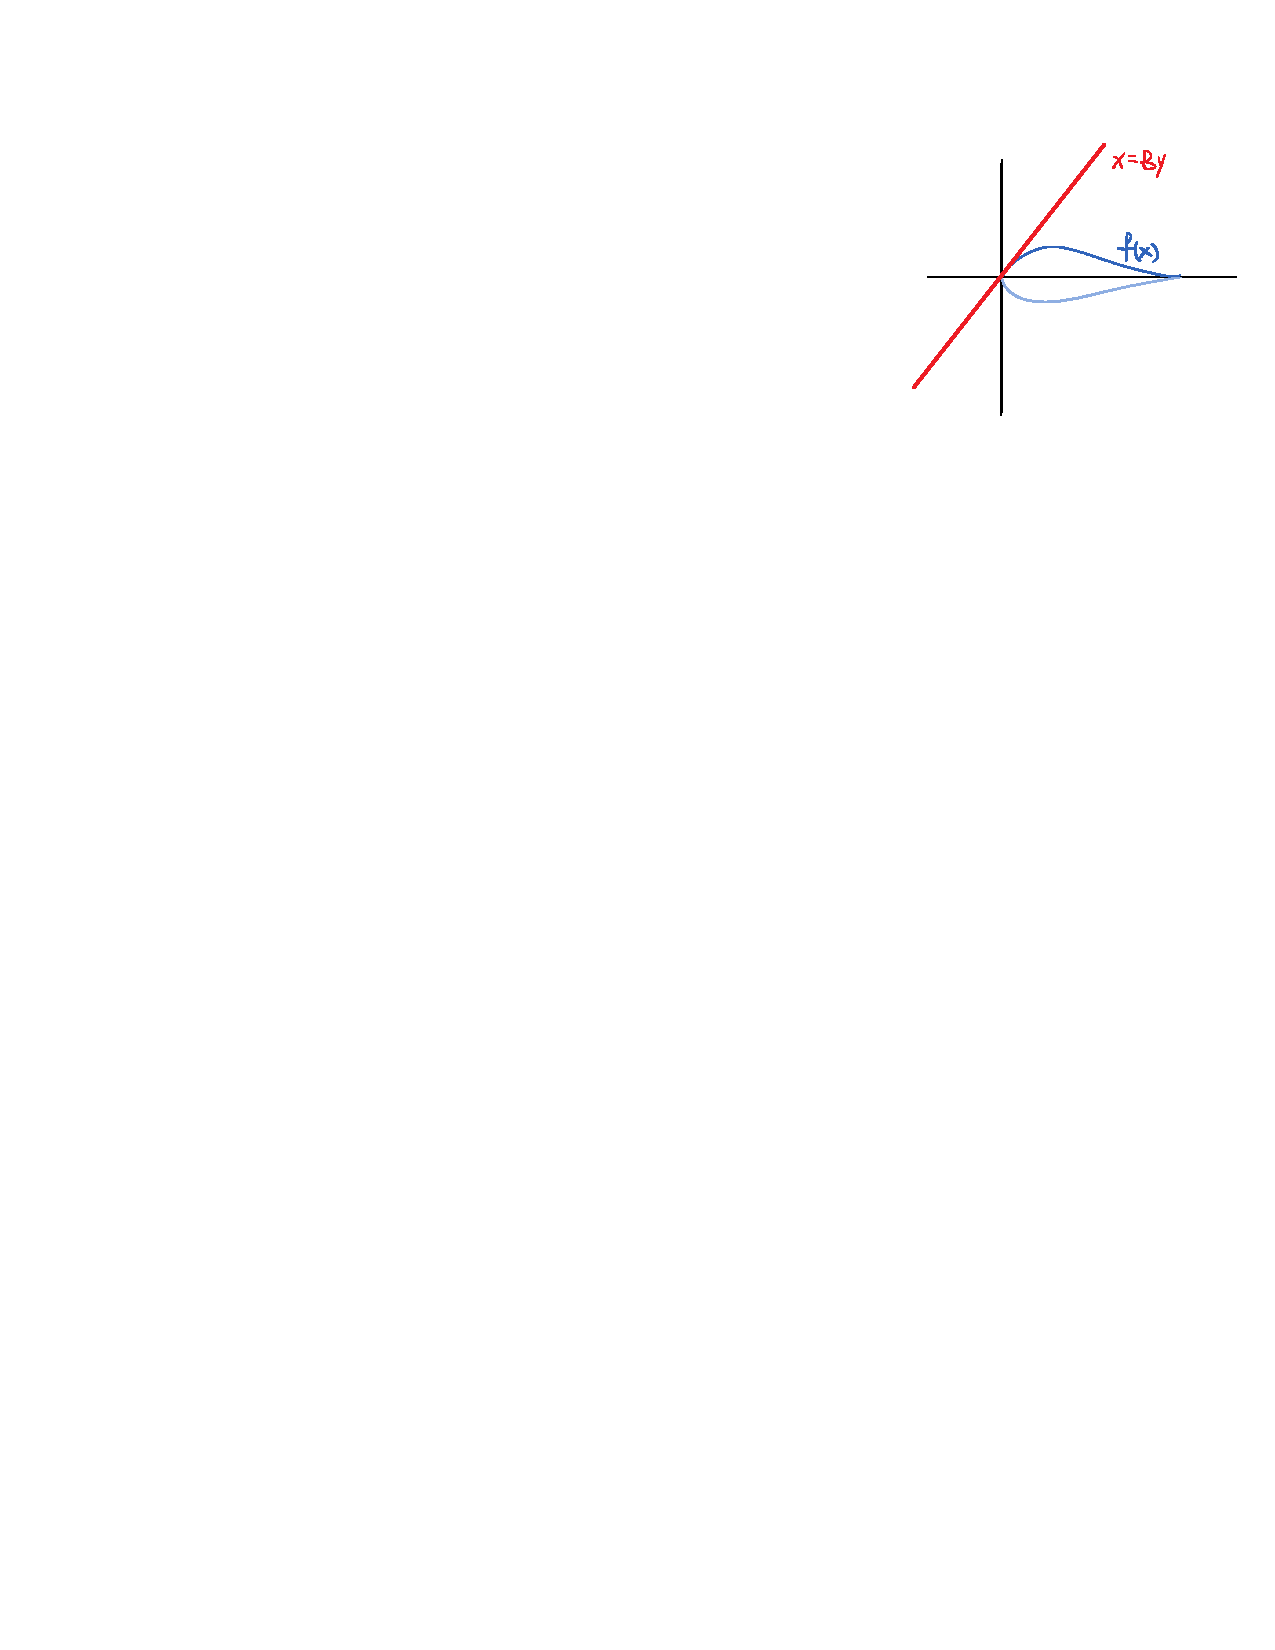
\includegraphics[scale=1.19]{foil.pdf}
\end{center}


On the top half region of the $xy$-plane, and on the left of the line $x = By$, simple argument can justify that $\phi = 0$ because we have $u_1 = 0$ and $v_1 = 0$ as the flow should be identical to that at the upstream negative infinity, hence on the left of the line $x= By$, we can write:
\begin{align*}
u=U \qquad\qquad v=0\qquad\qquad \phi=0
\end{align*}
On the line $x = By$, we should have the followings by the continuity of $\phi$:
\begin{align*}
\phi = 0 = F(0) + G(2x) \qquad \Rightarrow \qquad G = \text{constant}, \text{ so we set }G=0
\end{align*}
hence we get:
\begin{align*}
\phi = F(x-By) \qquad \qquad \left.\frac{\partial \phi}{\partial y}\right|_{y=0} = -BF'(x-0) = Uf'(x)
\end{align*}
solving for $F$, we get:
\begin{align*}
F(x) = -\frac{U}{B}f(x) \qquad\text{since }F(0) = 0, \ f(0) = 0
\end{align*}
that is, we get:
\begin{align*}
\phi = -\frac{U}{B}f(x-By)
\end{align*}
and hence:
\begin{align*}
v_1 = \frac{\partial \phi}{\partial y} = Uf'(x-By)
\end{align*}
For the bottom half of the $xy$-plane, one can apply a similar argument with the line $x = -By$ to get the pattern of the flow blow the $x$-axis. 
\newpage


\section[Shallow Water Waves]{\color{red}Shallow Water Waves\color{black}}
Consider shallow water waves, in terms of nonlinear theory. In the linear case, we have $c = \sqrt{gh_0}$ as discussed in the last section. Denote the height of the flow as $h(x,t)$, and let $L$ be half of the wavelength of the surface wave, and assume that we have $h(x,t) <<L$. In this case we can write the followings for momentum equations:
\begin{align*}
\frac{Du}{Dt} = -\frac{1}{\rho}\frac{\partial p}{\partial x} \qquad\qquad\qquad \frac{Dv}{Dt} = -\frac{1}{\rho}\frac{\partial p}{\partial y}-g
\end{align*}
Here we also consider incompressible flow:
\begin{align*}
\nabla \cdot \vec{u} = 0
\end{align*}
We also assume that the vertical acceleration is much less than the gravity, this assumption is based on experimental experiences, and here we write:
\begin{align*}
\frac{Dv}{Dt} \ll g 
\qquad \Rightarrow \qquad
 p(x,t) = -\rho gy + f(x,t)
\end{align*}
with boundary conditions $p= p_0$ at $y = h(x,t)$, we get:
\begin{align*}
p_0 = -\rho g h(x,t) + f(x,t) \qquad \Rightarrow \qquad f(x,t) = p_0 + \rho gh(x,t)
\end{align*}
hence we can solve for $p$:
\begin{align*}
p(x,t) = -\rho g y + p_0 + \rho gh(x,t) = p_0 - \rho g( y-h(x,t))
\end{align*}
Now we get:
\begin{align}
\frac{Du}{Dt} = -\frac{1}{\rho} \rho g \frac{\partial h}{\partial x} = -g \frac{\partial h}{\partial x}
\end{align}
where we see that $u$ is independent of $y$ if it initially is independent of $y$. WLOG, we assume that $u$ is independent of $y$ at $t=0$. For kinematic boundary condition in this system, we write the following at $y=h(x,t)$:
\begin{align}
\hat{n} = \frac{(-\frac{\partial h}{\partial x}, 1)}{\sqrt{1+\left(\frac{\partial h}{\partial x}\right)^2}} \qquad \Rightarrow \qquad v = \frac{\partial h}{\partial t} + n \frac{\partial h}{\partial x}  
\end{align}
On the other hand, we know that $\nabla \cdot n = 0$, hence we have:
\begin{align*}
\frac{\partial u}{\partial x} + \frac{\partial v}{\partial y} = 0 \qquad \Rightarrow \qquad v = -y \frac{\partial u}{\partial x} + f(x,t)
\end{align*}
where we use the fact that $\frac{\partial u}{\partial x}$ is independent of $y$. Also note here $f(x,t) = 0$ because $v = 0$ at the bottom surface $y = 0$. Hence now we get:
\begin{align}
v = -y \frac{\partial u}{\partial x}
\end{align}
Combining (3.21) and (3.20) with $y = h$, we can write the following:
\begin{align}
\frac{\partial h}{\partial t} + u \frac{\partial h}{\partial x} + h \frac{\partial u}{\partial x} = 0
\end{align}
By conservation of mass, we can write the following:
\begin{align*}
\Delta x \cdot \frac{\partial h}{\partial t} = \frac{\partial }{\partial t}\left(\text{volume of the small parcel}\right) =- \text{(net flux out)} = -h u|_{x+\Delta x} + h u|_x
\end{align*}
hence rearranging we have:
\begin{align*}
\frac{\partial h}{\partial t} = -\frac{\partial hu}{\partial x}
\end{align*}
From (3.19), we also get:
\begin{align}
\frac{\partial u}{\partial t}+ u \frac{\partial u}{\partial x} = -g\frac{\partial h}{\partial x}
\end{align}
assume that $\frac{\partial }{\partial x} \propto \frac{1}{L}$, $\frac{\partial}{\partial t} \propto u \cdot \frac{\partial}{\partial x}\propto \frac{U}{L}$, and $u\propto U $, then from (3.23) we see that we have:
\begin{align*}
\text{LHS of (3.22)} \propto \frac{U^2}{L}\propto \frac{gh}{L} \qquad \Rightarrow \qquad U \propto \sqrt{gh}
\end{align*}
on the other hand, from (3.21), we see that we have:
\begin{align*}
V\propto \frac{U}{L}h \qquad\qquad \frac{Dv}{Dt} \propto \frac{U^2}{L^2}h \propto \frac{gh^2}{L^2} \ll g
\end{align*}
this validate that $\frac{Dv}{Dt} \ll g$. Here (3.22) and (3.23) give us a set of PDE to solve:
\begin{align}
\begin{cases}
\frac{\partial u}{\partial t}+ u \frac{\partial u}{\partial x} +g\frac{\partial h}{\partial x} = 0\\
\frac{\partial h}{\partial t}+ u \frac{\partial h}{\partial x}+ h \frac{\partial u}{\partial x} = 0
\end{cases}
\end{align}
which can be solved using method of characteristics. Here we define:
\begin{align*}
c(x,t) = \sqrt{gh(x,t)} \qquad \Rightarrow \qquad h = \frac{c^2}{g}
\end{align*}
so we get:
\begin{align*}
\frac{\partial h}{\partial t} = \frac{2c }{g}\frac{\partial c}{\partial t} \qquad\qquad\qquad \frac{\partial h}{\partial x} = \frac{2c }{g}\frac{\partial c}{\partial x}
\end{align*}
combining with (3.24), we can write:
\begin{align*}
\begin{cases}
\frac{\partial u}{\partial t} + u \frac{\partial u}{\partial x} + 2c \frac{\partial c}{\partial x} = 0  \\
\frac{\partial 2c}{\partial t} + u \frac{\partial 2c}{\partial x} + c \frac{\partial u}{\partial x} = 0
\end{cases}
\end{align*}
rearranging we get:
\begin{align}
\begin{cases}
\left(\frac{\partial}{\partial t} + (u+c)\frac{\partial}{\partial x}\right)(u+2c)=0\\
\left(\frac{\partial }{\partial t}+(u-c) \frac{\partial }{\partial x}\right)(u-2c) = 0
\end{cases}
\end{align}
Let $C_1 = (x(s), t(s))$, such that we have:
\begin{align*}
\frac{dt}{ds} = 1 \qquad \frac{dx}{ds} = u+c \qquad\qquad \text{with}\ t(0) = t_0, \ x(0) = x_0
\end{align*}
Then (3.25) reads the following:
\begin{align}
\left(\frac{d t}{d s}\frac{\partial}{\partial t} + \frac{d x}{d s}\frac{\partial }{\partial x} \right)(u+2c) = 0 \qquad \Rightarrow \qquad \frac{d}{ds}(u+2c) = 0 \ \ \text{along }C_1
\end{align}
Similarly, for $C_2(x(s), t(s))$ defined by $\frac{dt}{ds} = 1$ and $\frac{dx}{ds} = u-c$, we get:
\begin{align}
\frac{d}{ds}(u - 2c) = 0 \ \ \text{along }C_2
\end{align}
\textbf{(C2)}\quad Here $C_2$ is in fact defined by a curve in the $xt$-plane with $\frac{dx}{dt} = u-c$.\\
\textbf{(C1)}\quad Similarly, $C_1$ is in fact defined by a curve in the $xt$-plane with $\frac{dx}{dt} = u+c$. \\
The curves defined in definitions (C1) and (C2) are called the characteristic curves. \\

\subsection*{Dam Break Problem}
Here we first consider a simple example where we have a dam break. The dam is positioned at $x=0$. At $t=0$, for $x<0$, the surface of the fluid is at constant height $h_0$, and for $x>0$, the height of the fluid surface is at constant $0$. At $t=0$, the dam is lifted, and fluid is free to flow. \\


Here, for $x<0$ and $t<0$, we have $u=0$, $c = \pm\sqrt{gh_0} = \pm c_0$. Hence the characteristics curves defined by $C_1$ and $C_2$ in the third quadrant of the $xt$-plane must satisfy $\frac{dx}{dt} = \pm c_0$. One can extend those characteristic curves $C_1$ and $C_2$ that lie in the third quadrant of the $xt$-plane into the region where $x < -c_0 t$ in the second quadrant of the $xt$-plane, and $C_1$ and $C_2$ in this region also satisfies $\frac{dx}{dt} = \pm c_0$, the same as in the third quadrant, according to (3.26) and (3.27). Now we call the third quadrant and the portion $x<-c_0 t$ in the second quadrant as region $P$, we call the rest of the second quadrant along with part of the first quadrant as region $Q$. 
\begin{center}
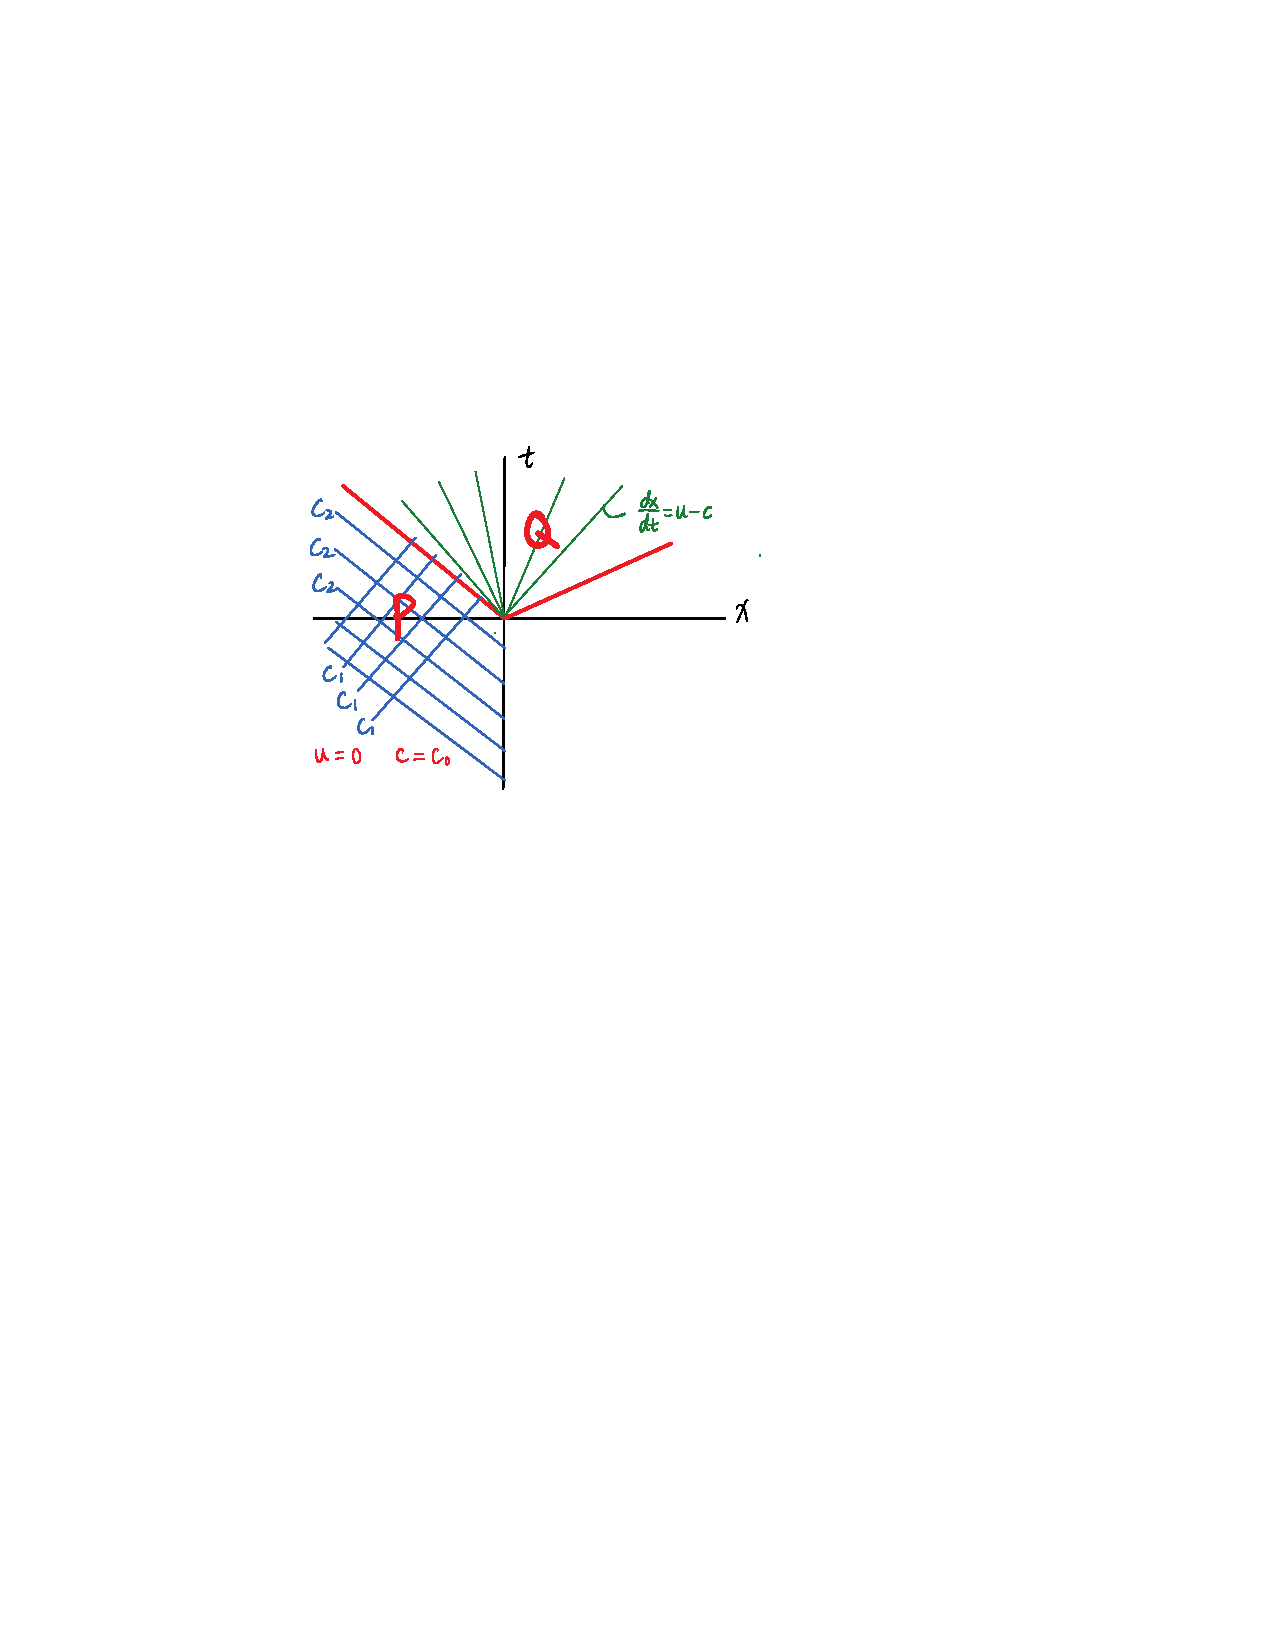
\includegraphics[scale=1.19]{QP.pdf}
\end{center}

What we are interested in is what happen in the region $Q$. In $Q$, none of the $C_2$ curves come from the third quadrant, then $\frac{dx}{dt} = -c_0$ is no longer true for the characteristic curves $C_2$ in this region. Along the curve $C_1$, we still have $u+2c = u_0+2c_0 = 2c_0 $ by (3.26), but $u$ and $c$ are no longer given by $u=0$ and $c = c_0$. Along the $C_2$ curves, we have $u-2c = k$ with $k \neq u_0-2c_0 = -2c_0$ by (3.27), and we have $k$ being different for different $C_2$ curves in region $Q$. Note that $C_2$ is defined by $\frac{dx}{dt} = u-c$, and since $u+2c$ is constant, $u-2c$ is constant, then $u, c$ are constant and hence we have:
\begin{align*}
\frac{dx}{dt} = u-c = \text{constant} = k' \qquad \Rightarrow \qquad x = k' t + b \ \ \ \text{along }C_2 \text{ in }Q
\end{align*}
To avoid characteristics curves intersecting in the region where $t>0$, we drop the term $b$ and look for solutions that satisfies $x = k't$:
\begin{align*}
\frac{x}{t} = u-c \qquad \text{along curves }C_2 \text{ in region }Q
\end{align*}
Also, for the $C_1$ curves in region $Q$:
\begin{align*}
u + 2c = 2c_0\qquad \text{along curves }C_1 \text{ in region }Q
\end{align*}
Solving for $u$ and $h=c^2/g$, we get the following solution for the problem:
\begin{align}
\begin{cases}
h=\frac{1}{g}\left( \frac{2}{3}c_0 - \frac{1}{3}\frac{x}{t}\right)^2 \\
u = \frac{2}{3}\left(c_0 + \frac{x}{t}\right)
\end{cases} \qquad\qquad \text{in region }Q
\end{align}
In region $P$, the solution for the problem is given by:
\begin{align*}
\begin{cases}
u = 0 \\
h =h_0
\end{cases} \qquad\qquad \text{in region }P
\end{align*}
Note that in region $Q$, at $x = 0$, we see that $h$ is invariant under time, and such wave in region $Q$ is called the rarefaction wave. \\

In region $Q$, where we call the rarefaction region, we have $u+2c = 2c_0$ along curves $C_1$, that is we can write $u = 2c_0 - 2c$, then we have:
\begin{align*}
\left(\frac{\partial}{\pd t}+(u-c) \frac{\pd}{\pd x}\right) (u-2c) = 0 \qquad \Rightarrow \qquad \left( \frac{\pd }{\pd t}+(2c_0 -3c)\frac{\pd}{\pd x}\right) (2c_0-4c) = 0
\end{align*}
define $z = -2c + 2c_0$, then we have:
\begin{align*}
\left( \frac{\pd}{\pd t} -z \frac{\pd}{\pd x}\right) (z+k) = 0
\end{align*}
where $k$ is a constant that we can drop when taking derivative, hence we have:
\begin{align}
\frac{\pd z}{\pd t } - z \frac{\pd z}{\pd x} = 0
\end{align}
Writing $z = F(\xi)$ with reasonable function $F$ and $\xi = x+zt$ would be one solution to (3.29). At the origin $x=0$, $t=0$, we have $h = \frac{4}{9}\, h_0$, and hence $c = \sqrt{gh} \Rightarrow \frac{2}{3}c_0 = c$, so $z = 0$ at the origin. Concluding, we say that, points on the wave surface characterized by positive $z$ move to the left, that is towards the negative $x$-direction, and larger positive $z$ move to the left faster. For points on the surface characterized negative $z$, the points move to the right, and faster when $z$ is more negative.  \\

\subsection*{Formation of a bore and hydraulic jump}
Suppose that the fluid of uniform depth $h_0$ is contained at rest in $x>0 $ by a vertical plate, and at $t=0$, the plate is started into motion in the positive $x$-direction with speed $U = \alpha t$, where $\alpha$ is a positive constant, We may again use the method of characteristics and an identical argument to that in the dam break problem leads to the following implicit solution:
\begin{align*}
z = f(x-zt) \qquad\qquad\qquad z= 3c-2c_0
\end{align*}
and again, points on the fluid surface characterized by positive $z$ moves to the right, with larger magnitude being faster. In this problem the slope of the surface at some point will eventually get to infinite, in which case a hydraulic jump occurs. Details of this discussion can be found in section 3.9 and 3.10 on \textit{Acheson}. \\

\subsection{$1$-dimensional gas flow}
Taking about gas with initial pressure $\rho_0$ and initial density $p_0$, being compressible, we obtain the followings for ideal gas:
\begin{align}
\rho\left( \frac{\partial u}{\partial t} + u \frac{\partial u}{\partial x}\right) = -\frac{\partial p}{\partial x} \qquad\qquad\quad \frac{\pd \rho}{\pd t} + \frac{\pd }{\pd x}(\rho u) = 0 \qquad\qquad\quad p\rho^{-\gamma} = p_0 \rho_0^{-\gamma}
\end{align}
Consider one situation, similar to the dam break problem, where we have a plate separating a region of gas with density $\rho = \rho_0$, and a region with lower density $\rho = 0$, or another situation where the vertical plate is pushing to the right starting at $t=0$ and the region has initially density $\rho = \rho_0$. In both situations, we can define $a^2 = \gamma p / \rho$, using (3.30) we get the followings:
\begin{align*}
\left( \frac{\pd}{\pd t}+ (u+a) \frac{\pd}{\pd x}\right) \left(u+ \frac{2a}{\gamma - 1}\right) = 0 \qquad\qquad\qquad \left( \frac{\pd}{\pd t}+ (u-a) \frac{\pd}{\pd x}\right)\left( u - \frac{2a}{\gamma-1}\right) = 0
\end{align*}
where we see that, for shallow water flow, we have $c = \sqrt{gh}$ in the equations to be solved, and in this $1$-dimensional gas flow, we have $a = \sqrt{\gamma p/\rho}$. The two systems are very analogues to each other.\\

Note that by including the viscosity of the flow, the shock, or the hydraulic jump that was mentioned previously, will be smoothed out, and leads to the steady traveling wave solution:
\begin{align*}
u(x,t) = \frac{U_1}{1+e^{\frac{x-vt}{\Delta}}}
\end{align*}  
where we have:
\begin{align*}
\Delta = \frac{8}{3}\frac{\nu}{(\gamma+1)U_1} \qquad\qquad\qquad V = a_0 + \frac{1}{4}(\gamma+1) U_1
\end{align*}
Details of this section can be found in section 3.11 on \textit{Acheson}. 

\newpage
\chapter{Potential Flow Theory}
\setcounter{section}{8}
In this chapter, we focus on a $2$-dimensional flow with Reynolds number approaching infinity, and we focus on irrotational where we have $\vec{\omega} = \nabla \times \vec{u} = 0$. \\

Let $\vec{u}$ be a velocity field of a $2$-dimensional flow, that is, $\vec{u} = (u,v,0)$. The real velocity potential $\phi$ is something that exists only if we have $\nabla \times \vec{u} = 0$, and hence is defined at any point $P$ in the fluid by:
\begin{align*}
\phi = \int_O^P \vec{u}\cdot d\vec{x}
\end{align*}
where $O$ is the origin in our problem. Here $\phi$ is independent of path in a simply-connected fluid region. That is, for paths $C_1$ and $C_2$ connecting the same end points and enclose a region $R$, we have:
\begin{align*}
\int_{C_1} \vec{u}\cdot d\vec{x} - \int_{C_2} \vec{u}\cdot d\vec{x} = \int_R 0\, dA = 0
\end{align*}
The circulation of the flow, as mentioned earlier, is defined to be the following, with $C$ being a path enclosing an air foil:
\begin{align*}
\Gamma  = \oint_C \vec{u}\cdot d\vec{x}
\end{align*}
note that $\Gamma$ may be nonzero in irrotational flow in a doubly-connected domain. \\

Here for simplicity, one might write $\vec{u} = (u,v)$, and we let $\omega = |\vec{\omega}| = \nabla \times (u,v,0)$.
\begin{defn}
The stream function of an incompressible $2$-dimensional flow. denoted as $\psi$, is defined to be the following integral:
\begin{align*}
\psi \coloneqq \int_O^P \vec{u}^{\perp} \cdot dx = \int_O u\,dy-v\,dx
\end{align*}
\end{defn}

For $\psi$ to be path independent, we must have:
\begin{align*}
\nabla^{\perp}\cdot \vec{u}^{\perp} = \left(- \frac{\partial}{\partial y}, \frac{\partial }{\partial x}\right) \cdot \left(-v, u\right) = \nabla \cdot \vec{u} =0 
\end{align*}
where we define:
$$\nabla^{\perp} \coloneqq \left( -\frac{\partial}{\partial y}, \frac{\partial}{\partial x}\right)$$ 
That is we have incompressible flow if and only if the stream function is independent of the path.

\begin{defn}
If a flow is incompressible and irrotational, then the flow is called a potential flow. 
\end{defn}
Since streamlines are tangent to the flow velocity vector of the flow, and one can easily check that $(\vec{u}\cdot \nabla) \psi = 0$, and with the following holds:
\begin{align*}
 \frac{d}{dt} \left(\psi(\gamma(t))\right) = \nabla \psi \cdot \gamma'(t) = \nabla \psi \cdot \vec{u}(t) = (\vec{u}\cdot \nabla) \psi = 0
\end{align*}
where $\gamma(t)$ is a streamline in the flow, hence the value of the stream function must be constant along a streamline. For $2$-dimensional potential flow, streamlines are perpendicular to equipotential lines. \\

Note that, for $2D$-flow, we can write the followings:
\begin{align*}
\phi = \int_O^P u\, dx + v\, dy \qquad \Rightarrow \qquad u = \frac{\partial \phi}{\partial x} \qquad v = \frac{\partial \phi}{\partial y} \qquad \vec{u} = \nabla \phi
\end{align*}
\begin{align*}
\psi = \int_O^P -v \, dx + u\, dy \qquad \Rightarrow \qquad v = -\frac{\partial \psi}{\partial x} \qquad u = \frac{\partial \psi}{\partial y}
\end{align*}
that is for potential flow, we have:
\begin{align*}
-\frac{\partial \psi}{\pd x} = \frac{\pd \phi}{\pd y} \qquad\qquad \qquad \frac{\pd \psi}{\pd y} = \frac{\pd \phi}{\pd x}
\end{align*}
satisfying the Cauchy-Riemann equations, so $w \coloneqq \phi + i\psi$ is an analytic function of $z = x+iy$. Note here also:
\begin{align*}
0 = \nabla \cdot\vec{u} = \frac{\pd u}{\pd x}+ \frac{\pd v}{\pd y} = \frac{\pd^2 \phi}{\pd x^2} + \frac{\pd \phi^2}{\pd y^2} = \nabla^2 \phi
\end{align*}
\begin{align*}
0 = \nabla^\perp \cdot \vec{u} = -\frac{\pd u}{\pd y}+\frac{\pd v}{\pd x} = -\frac{\pd^2 \psi}{\pd y^2} - \frac{\pd^2 \psi}{\pd x^2} = -\nabla^2 \psi
\end{align*}
Since $w$ is analytic, we can write the following:
\begin{align*}
\frac{dw}{dz } = \frac{\partial w}{\partial x} = \frac{\partial w}{i \partial y} = \frac{\partial}{\partial x}\left( \phi + i\psi\right) = u-iv = \text{conjuagate velocity} = \text{complex velocity}
\end{align*}
and here $w(z)$ defines the complex potential. Note that we can also write:
\begin{align*}
\frac{dw}{dz} = \frac{\partial}{i \partial y}(\phi+i \psi) = \frac{\partial \psi}{\partial y} - i\frac{\partial \phi}{\partial y}
\end{align*}
\example Consider the flow defined by $u = U \cos(\alpha)$ and $v = U \sin(\alpha)$. Then we have:
\begin{align*}
\frac{dw}{dz} = \overline{u + iv} = \overline{U e^{i\alpha}} = U e^{-i\alpha}
\end{align*}
and hence we have:
\begin{align*}
w = U e^{-i\alpha}z = U \left( x\cos(\alpha)+y \sin(\alpha)\right)+i U(-x\sin(\alpha) + y \cos(\alpha)) 
\end{align*}
and here:
\begin{align*}
\phi = U (x\cos(\alpha) + y \sin(\alpha)) \qquad\qquad\qquad \psi = U(-x\sin(\alpha) + y \cos(\alpha))
\end{align*}


\newpage
\example For $2$-dimensional flow cylindrical coordinate, we have:
\begin{align*}
\nabla  = \left( \frac{\partial}{\partial r} ,  \frac{1}{r}\frac{\partial}{\partial \theta}\right)
\end{align*}
Consider the line vortex flow $\vec{u} = \frac{\Gamma}{2\pi r}\vec{e}_{\theta}$:
\begin{center}
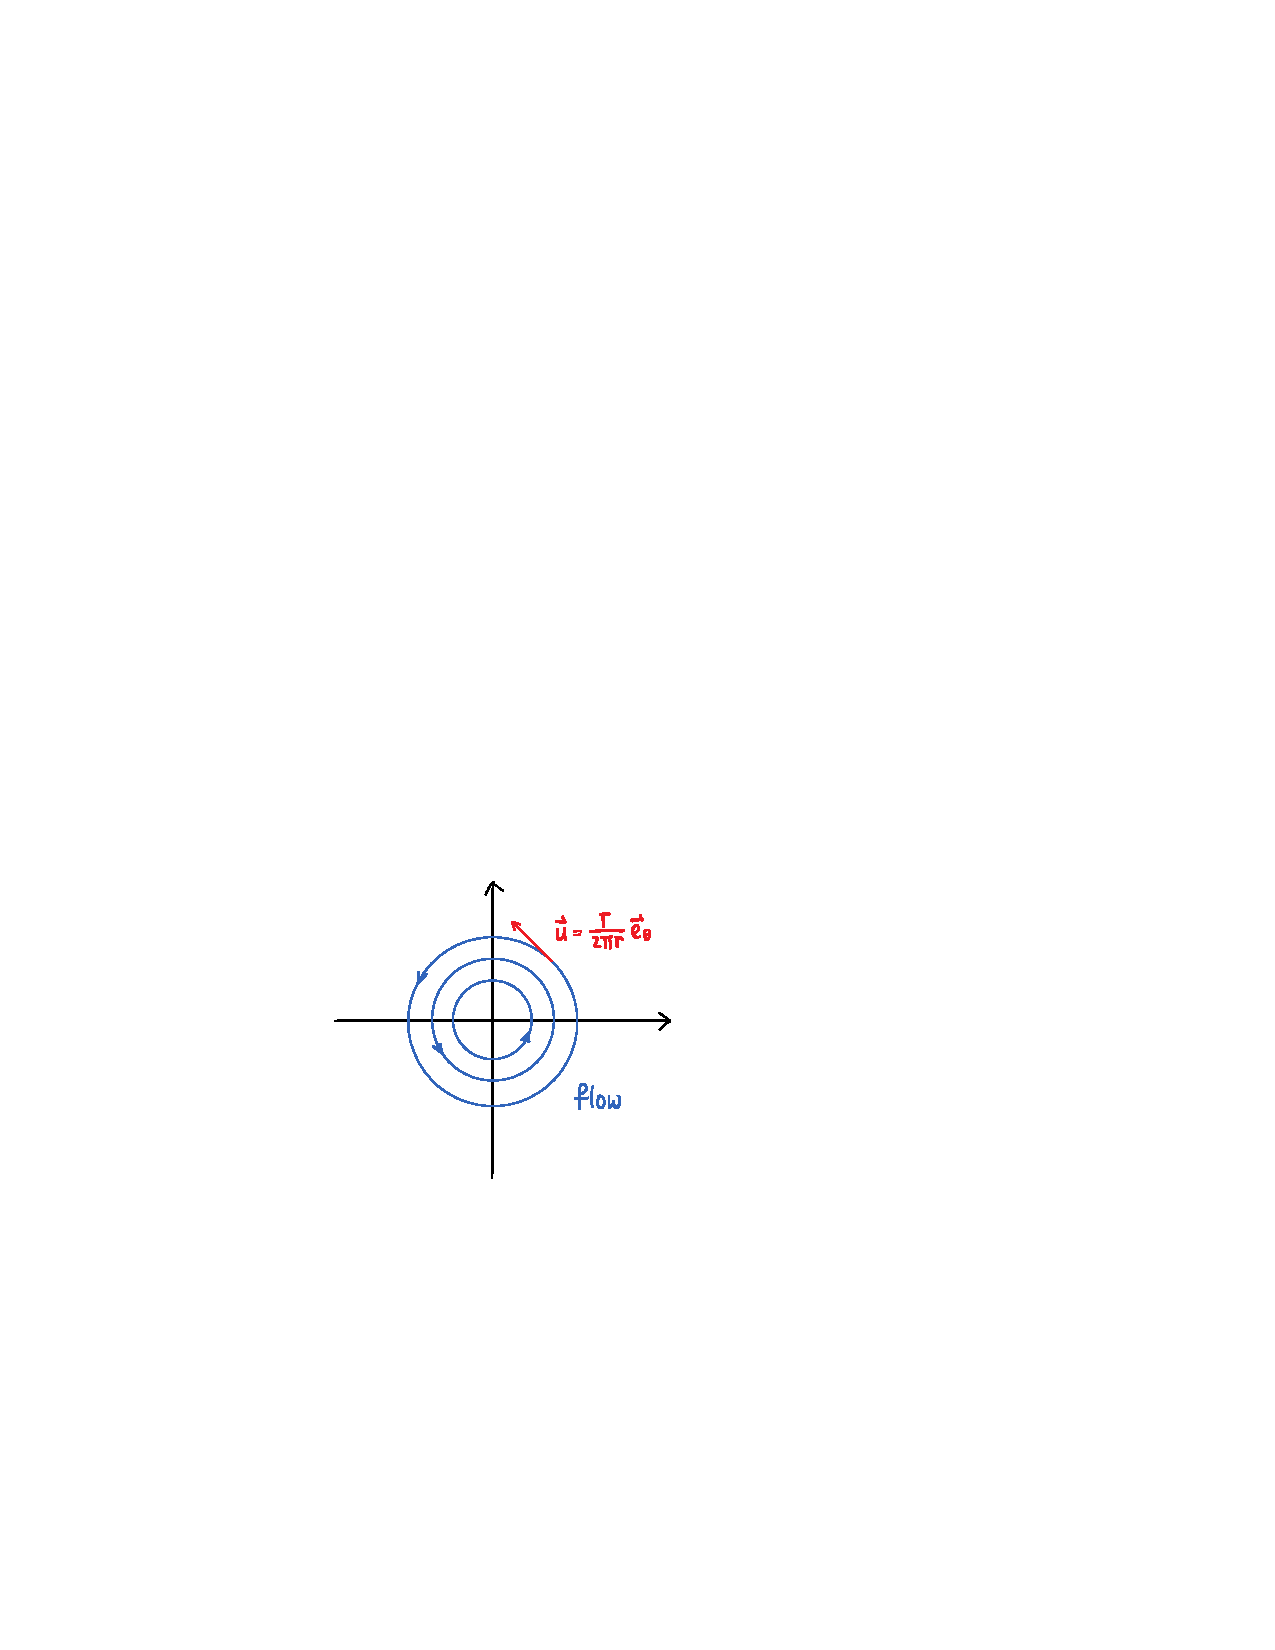
\includegraphics[scale=1.19]{vortex.pdf}
\end{center}

Then we see that we have:
\begin{align*}
u_{\theta} = \frac{1}{r}\frac{\partial \phi}{\partial \theta} = \frac{\Gamma}{2\pi r} \qquad\Rightarrow \qquad \phi = \frac{\Gamma}{2\pi}\theta+\text{constant}
\end{align*}
here we omit the constant term, hence we write $\phi = \frac{\Gamma}{2\pi}\theta $. Moreover, we have:
\begin{align*}
(-u_{\theta}, u_r) = \left( \frac{\partial \psi}{\partial r}, \frac{1}{r}\frac{\partial \psi}{\partial \theta}\right)
\end{align*}
then we have:
\begin{align*}
-\frac{\partial \psi}{\partial r} = \frac{\Gamma}{2\pi r} \qquad \Rightarrow \qquad \psi = -\frac{\Gamma}{2\pi}\log(r) + \text{constant}
\end{align*}
and again, we omit the constant term, that is $\psi =  -\frac{\Gamma}{2\pi}\log(r) $. Now we have:
\begin{align*}
w = \phi + i\psi = \frac{\Gamma}{2\pi}\left( \theta - i \log(r)\right) = \frac{\Gamma}{2\pi i}( \log(r) + i\theta) = \frac{\Gamma}{2\pi i}\log(re^{i\theta}) = \frac{\Gamma}{2\pi i}\log (z)
\end{align*}
Here we can also see that the streamlines are described by where $r$ is constant.


\hfill\break
\hfill\break
\example \textbf{Flows in and around wedges}\\
Consider a flow defined by $w = Az^n = Ar^n \cos(n \theta) + i Ar^n \sin(n \theta) = \phi + i\psi$. \\
Hence we have $\psi = 0$ for $\theta = m\frac{\pi}{n}$. For $n=2$, we see that we have:
\begin{align*}
\psi = Ar^2 \sin(2\theta) = \text{constant} = 2Ar^2 \sin(\theta) \cos(\theta) = 2A xy
\end{align*}
hence for $n=2$, the stream lines are characterized by the following:
\begin{align*}
y = \frac{\text{constant}}{2Ax}
\end{align*}

For $n = 1/2$, we have:
\begin{align*}
\psi = r^{1/2}\sin(\theta/2) = r^{1/2}\sqrt{\frac{1-\cos(\theta)}{2}} = \text{constant} \quad \Rightarrow \quad r\left( \frac{1-\cos(\theta)}{2}\right) = \text{constant}
\end{align*}
hence for $n=1/2$, the stream lines are characterized by the following:
\begin{align*}
\sqrt{x^2 + y^2 }-x = \text{constant}
\end{align*}
The speed of the flow at the origin is given by the following:
\begin{align*}
||\vec{u}|| = \left|\frac{dw}{dz}\right| = \left|u-iv\right| = \sqrt{u^2 + v^2} = |An z^{n-1}| = \begin{cases}
0 & \text{at }z=0, \ n>1\\
\infty &\text{at }z=0, \ n<1
\end{cases}
\end{align*}


\newpage
\section[Method of Images]{\color{red} Method of Images\color{black}}
Consider a vertical boundary at the line $x=0$. There is a vortex on the right with distance $d$ from the boundary, counterclockwise orientation. The flow is suppose to have zero velocity along the $x$-direction when it meets the boundary, hence one can place an imaged vortex at distance $d$ to the left of the boundary, clockwise direction, to create a symmetry such that the flow along the boundary at $x=0$ does not penetrate the boundary. In which case, the system reads:
\begin{align*}
-\nabla^2 \psi &= 0 \qquad\qquad\text{with }\psi = \text{constant along the boundary}\\
\nabla^2 \phi &= 0 \qquad\qquad\text{with }\frac{\partial \phi}{\partial n} = 0\text{ on the boundary}
\end{align*}
where $n$ denote the normal of the boundary. Now we can write the following:
\begin{align*}
w = \frac{\Gamma}{2\pi i}\log(z-d)  - \frac{\Gamma}{2\pi i}\log(z+d) = \frac{\Gamma}{2\pi i}\log\left( \frac{z-d}{z+d}\right) = \frac{\Gamma}{2\pi i}\left( \log\left|\frac{z-d}{z+d}\right| + i \text{arg}\left( \frac{z-d}{z+d}\right)\right)
\end{align*}
Hence we have:
\begin{align*}
\psi = -\frac{\Gamma}{2\pi}\log\left|\frac{z-d}{z+d}\right| = 0 \text{ on the boundary defined at }x=0 
\end{align*}
If one instead has a circular boundary of radius $a$ centered at the origin, and a vortex placed at a distance $r$ from the origin, at position $z_0 = re^{i\theta}$. Then we can place an imaged vortex at a distance $a^2/r$ from the origin, at position $a^2 / \bar{z}_0= (a^2/r)e^{i\theta}$, such that the circular boundary is a streamline of the flow generated by the vortex at $re^{i\theta}$. Note that, in such case, when $r$ approaches infinity, the imaged vortex is placed equivalently at the origin. To show that the circular boundary is a streamline, we write the following:
\begin{align}
w = \frac{\Gamma}{2\pi i}\log(z - z_0) - \frac{\Gamma}{2\pi i}\log\left( z - \frac{a^2}{z_0}\right) = \frac{\Gamma}{2\pi i}\log\left( \frac{z-z_0}{z- a^2/z_0}\right)
\end{align}
and hence the stream function is given by:
\begin{align*}
\psi = -\frac{\Gamma}{2\pi}\log\left|\frac{z-z_0}{z-a^2/z_0}\right| = \text{constant}
\end{align*}
At the circular boundary, we have $z\bar{z} = |z|^2 = a^2$, and hence we have:
\begin{align*}
\left|z - \frac{a^2}{z}\right| = \left|z - \frac{z\bar{z}}{z_0}\right| = |z| \cdot \left|1 - \frac{\bar{z}}{\bar{z}_0}\right| = \frac{|a|}{|z_0|}\left|z_0 - z\right|
\end{align*}
hence, at the boundary $|z| = a$, we get:
\begin{align*}
\psi = -\frac{\Gamma}{2\pi}\log\left| \frac{z_0}{a}\right| = \text{constant} \qquad \qquad \text{at the boundary}
\end{align*}
this shows that the circular boundary is indeed a steamline of the flow. \\



\begin{thm}[Milne-Thomson Circle Theorem]
Consider $f(z)$ which has all singularities lie in $|z| >a$. We define the complex velocity of a flow as the following:
\begin{align*}
w = f(z) + \overline{f\left(a^2 / \bar{z}\right)}
\end{align*}
Then the complex velocity $w$ defines a flow with the same singularities as $f$ in the region $|z|>a$, and has $|z| = a$ as a streamline. 
\end{thm}
\begin{proof}
Let $z_0$ be a singularity of $f$ with $|z_0|>a$, then we know that we have:
\begin{align*}
\left| \frac{a^2}{\bar{z}_0}\right| < a
\end{align*}
hence all singularities of $\overline{f(a^2/\bar{z})}$ lie inside $|z| = a$. Now let $|z| = a$, then we can write the following:
\begin{align*}
z\bar{z} = a^2 \qquad \Rightarrow \qquad w(z) = f(z) + \overline{f(z\bar{z}/\bar{z})} = f(z) + \overline{f(z)} \in \R
\end{align*} 
and hence at $|z| = a$, we have $\psi=0$, giving us a streamline. 
\end{proof}


Hence we see that the previous example is a special case with $f(z) = \frac{\Gamma}{2\pi i}\log(z-z_0)$, and writing the following also gives us a solution to the problem:
\begin{align}
w = \frac{\Gamma}{2\pi i}\log(z-z_0) + \overline{ \frac{\Gamma}{2\pi i}\log\left( \frac{a^2}{\bar{z}} - z_0\right) } = \frac{\Gamma}{2\pi i}\log(z-z_0) - \frac{\Gamma}{2\pi i}\log\left( \frac{a^2}{\bar{z}} - z_0\right) 
\end{align}
Here (4.2) differs from (4.1) by a term, which suggests that solution to the problem is not unique. 



\newpage
\section[Flow Past an Ellipse]{\color{red}Flow Past an Ellipse\color{black}}
First we consider the simple case where the ellipse is a perfect cylinder that has radius $a$, with axis parallel to the $z$-axis, one can describe the complex potential as the following:
\begin{align*}
w(z) = f(z) = Uz = f(z) + \overline{f\left( a^2/\bar{z}\right)} = Uz + U\frac{a^2}{z}
\end{align*}
One can also add a term representing a point vortex at the origin, while stile have $|z| = a$ being a streamline:
\begin{align*}
w(z) =  Uz + U\frac{a^2}{z} + \frac{\Gamma}{2\pi i}\log(z)
\end{align*}
If $\Gamma = 0$, here we can write:
\begin{align*}
\phi|_{z = re^{i\theta}} = \Re(w|_{z = re^{i\theta}}) = Ur\cos(\theta) + U \frac{a^2}{r}\cos(\theta) = U\left( r + \frac{a^2}{r}\right) \cos(\theta)
\end{align*}
hence we can write:
\begin{align*}
u_{\theta} = \frac{1}{r}\frac{d\phi}{d\theta} = -U \left( 1+ \frac{a^2}{r^2}\right) \sin(\theta)
\end{align*}
on the body of the cylinder, $r=a$, and we have:
\begin{align*}
u_{\theta}  = -2U \sin(\theta) 
\end{align*}

If $\Gamma \neq 0$, one can compute and get the following:
\begin{align*}
u_{\theta} = -U \left( 1+ \frac{a^2}{r^2}\right) \sin(\theta) + \frac{\Gamma}{2\pi r}
\end{align*}
Here we define:
\begin{align*}
B = -\frac{\Gamma}{2\pi Ua}
\end{align*}
which is related to the last term in $U_\theta$. \\
Different values of $B$ gives us different shapes of the flow:
\begin{center}
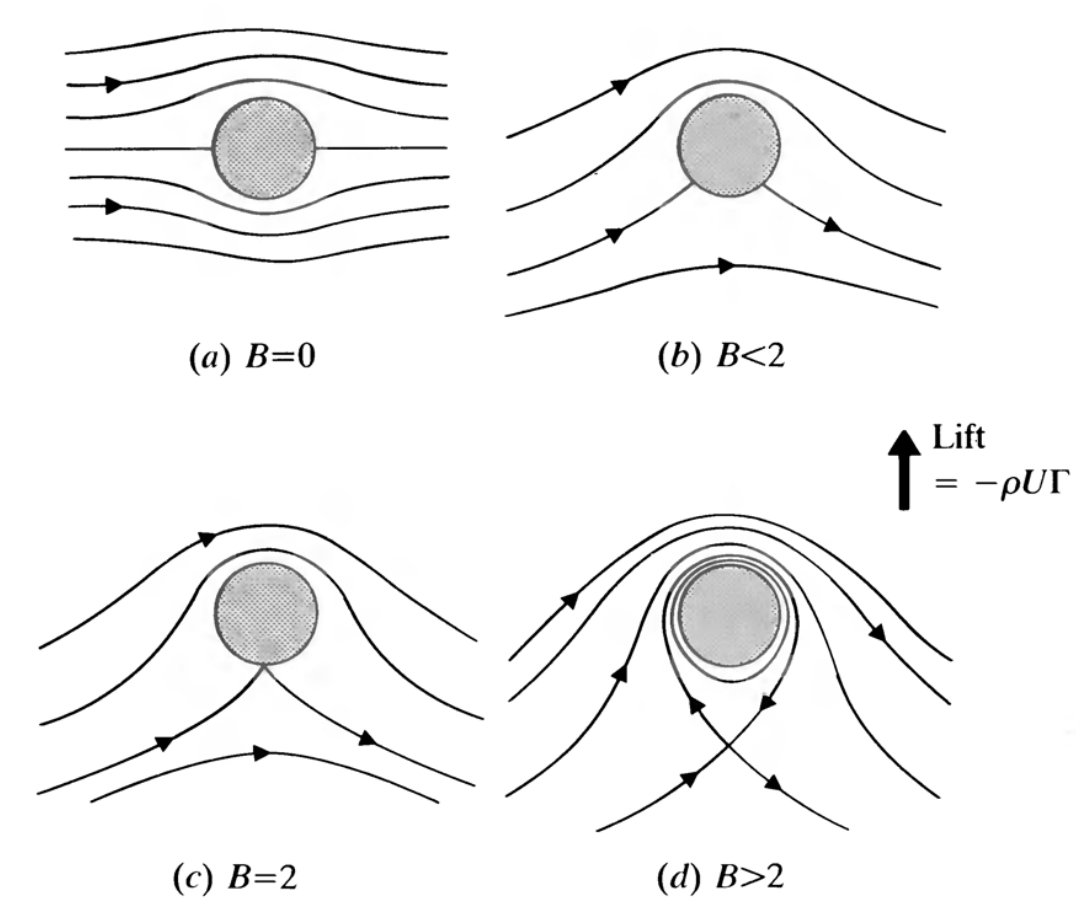
\includegraphics[scale=0.35]{B.png}\\
\color{gray}(Fig 4.4 on \textit{Acheson})\color{black}
\end{center}

Now calculate the force on the cylinder using the Bernoulli's equation for steady flow:
\begin{align*}
p + \frac{1}{2}\rho |\vec{u}|^2 = \text{constant} \qquad\qquad \text{on }r=a
\end{align*} 
On the surface of the cylinder, $u_r = 0$, hence rearranging we can write the following:
\begin{align*}
\frac{p}{\rho} = \text{constant} - \frac{1}{2}u_{\theta}^2|_{r=a}
\end{align*}
suppressing all constants as $K$, we can write the following:
\begin{align*}
\frac{p}{\rho} 
&= K - \frac{1}{2}\left( -2U \sin(\theta) + \frac{\Gamma}{2\pi a}\right)^2 \\
&= K - 2U^2 \sin^2(\theta) + \frac{\Gamma U}{\pi a} \sin(\theta) \\
&= K-U^2(1-\cos(2\theta)) + \frac{\Gamma U}{\pi a}\sin(\theta)
\end{align*}
Hence the force can be computed via:
\begin{align}
\vec{F}=(F_x, \ F_y) = \int_{r= a} = -p\, \hat{n}_{out}\, ds
\end{align}
where $\hat{n}_{out}$ is the normal vector on the surface of the cylinder, and we have:
\begin{align*}
\hat{n}_{out} = \bmat{\cos(\theta) \\ \sin(\theta)} \qquad\qquad ds = a\,d\theta
\end{align*}
computing the integral (4.3), we get the following:
\begin{align*}
\text{Drag} &\coloneqq F_x = \int_0^{2\pi } -p \cos(\theta) \cdot a\, d\theta = 0\\
\text{Lift}&\coloneqq F_y = \int_0^{2\pi} -p \sin(\theta) \cdot a \, d\theta = \frac{\rho \Gamma Ua}{\pi a}\frac{2\pi}{2} = -\rho U \Gamma
\end{align*}
where we have:
\begin{align*}
\Gamma = \oint_C \vec{u}\cdot d\vec{x}
\end{align*}
with $C$ being a counterclockwise path enclosing the body. If $\vec{u}$ is coming from the left, the lift on the body will be upwards as $\Gamma$ is negative in such case.\\


\subsection{Conformal mapping between spaces}
Suppose $w(z) = \phi + i\psi$ is a complex potential in the $z$-plane, or a complex analytic function. Here we let $Z = f(z) $ be a complex analytic function with an inverse $z = F(Z)$. Then the composition $w(F(Z)) \coloneqq W(Z)$ is also an analytic function of $Z$, which is a complex potential in the $Z$-plane. \\

Here we take the complex potential $w(z)$ for flow past an object $\M$ in the $z$-plane. Then we conformally map the object $M$ to a new object $\M'$ via the analytic function $Z = f(z)$, whose inverse is $z = F(Z)$. The flow past the new object is then given by $W(Z) = w(F(Z))$. \\

\example\\ 
Say the flow around a cylinder $\M$ with axis aligned with the $z$-axis is given by:
\begin{align*}
w(z) = U \left( z + \frac{a^2}{z}\right)
\end{align*}
and consider the new object $\M'$ is mapped by the following function:
\begin{align}
Z = f(z) = z+ \frac{c^2}{z} \tag{Joukowski map}
\end{align}
one can immediately observe that, the new flow, if we have $c= a$, is defined by:
\begin{align*}
W(Z) = UZ \qquad\qquad c=a
\end{align*}
Note that the boundary of $\M$ is defined by:
\begin{align*}
\partial \M = \{ae^{i\theta}\mid 0\leq \theta < 2\pi\}
\end{align*}
and hence the boundary of $\M'$ is defined by the following:
\begin{align*}
\partial \M' = \left\{f(ae^{i\theta}) = ae^{i\theta}+\frac{c^2}{a}e^{i\theta} \mid 0\leq \theta < 2\pi\right\}
\end{align*}
where we have:
\begin{align*}
f(ae^{i\theta}) = ae^{i\theta}+\frac{c^2}{a}e^{i\theta} = \left( a+ \frac{c^2}{a}\right) \cos(\theta) + i \left( a - \frac{c^2}{a}\right) \sin(\theta)
\end{align*}
which describes an ellipse in Cartesian coordinate: 
\begin{align*}
\left\{\left(\left( a+ \frac{c^2}{a}\right) \cos(\theta)  , \left( a - \frac{c^2}{a}\right) \sin(\theta)\right)\mid 0\leq \theta < 2\pi\right\}
\end{align*}
Moreover, we can write the following:
\begin{align*}
z = F(Z) = \frac{Z}{2}\pm \sqrt{\frac{Z^2}{2} - c^2}
\end{align*}
Hence we have:
\begin{align*}
W(Z) = U \left( \frac{Z}{2}\sqrt{\frac{Z^2}{4} - c^2} + \frac{a^2}{Z/2 \pm \sqrt{Z^2/4-c^2}}\right)
\end{align*}
and here $Z$-plane is where $\M'$ lies in. 

\subsection*{Flow at angle $\alpha$ past a cylinder}
In this case, we write the parallel flow as $w(z) = U ze^{-i\alpha}$, in which case the velocity is defined by $\overline{dw/dz} = Ue^{i\alpha}$. And hence the flow past past the cylinder is given by:
\begin{align*}
w(z) = Uze^{-i\alpha} + U \overline{\left( a^2/\bar{z} e^{-i\alpha}\right)} = U \left( ze^{-i\alpha} + \frac{a^2}{z}e^{i\alpha}\right)
\end{align*}
Through the Joukowski map, we let $Z = z+ c^2/z$ to get an ellipse. For flat plate, one can find the velocity of the flow at the two edges of the plate is infinite, while the velocity of the flow around an ellipse is always finite. 
\begin{center}
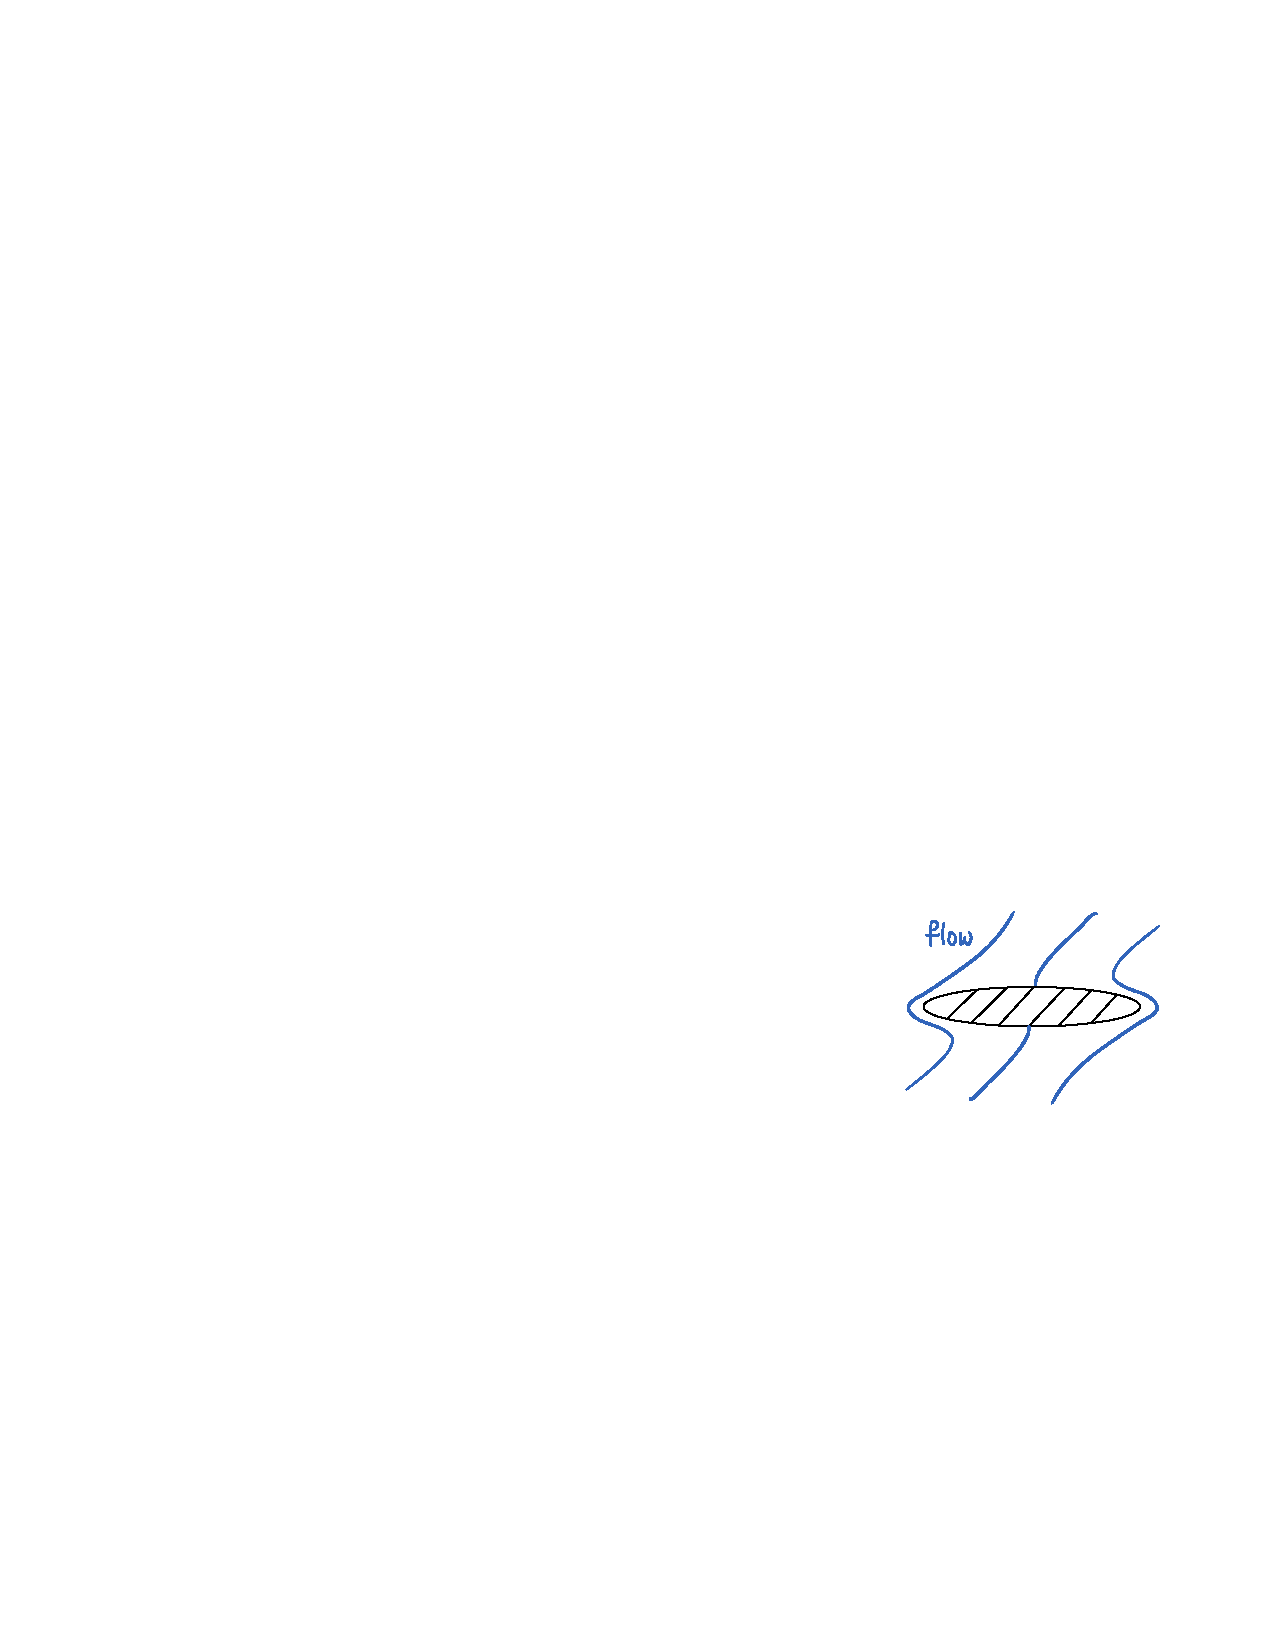
\includegraphics[scale=1.19]{ellipse.pdf}
\end{center}

Here again, we can add a vortex of strength $\Gamma$:
\begin{align*}
w(z) = U \left( ze^{-i\alpha} + \frac{a^2}{z}e^{i\alpha}\right) + \frac{\Gamma}{2\pi i}\log(z)
\end{align*}
The Kutta condition is to choose $\Gamma$ to remove the velocity singularity at the trailing edge of the plat plate, or other shapes such as the Joukowski air foil. Note that we can write the following to find the velocity field of the flow around a flat plate, where we assume that we have $c=a$:
\begin{align*}
\frac{dW}{dZ} = u_* - iv_* = \frac{dw}{dz}\frac{dz}{dZ} = \frac{dw/dz}{dZ/dz} = \frac{U\left( e^{i\alpha} - \frac{a^2}{z^2}e^{i\alpha}\right) +\frac{\Gamma}{2\pi i}\frac{1}{z}}{1-\frac{a^2}{z^2}}
\end{align*}
hence the velocity is infinite at $z = \pm a$, or $Z = \pm 2a$, if the term $\frac{\Gamma}{2\pi i}\frac{1}{z}$ were to be neglected. However, one can choose $\Gamma$ such that the numerator is $0$ at $z = a$, that is:
\begin{align*}
U(e^{-i\alpha} - e^{i\alpha}) + \frac{\Gamma}{2\pi i}\frac{1}{a} = 0 \qquad \Rightarrow \qquad \Gamma = -4\pi Ua \sin(\alpha)
\end{align*}
hence removing the singularity at $z=a$, that is the velocity is now finite at the trailing edge. We can also remove the singularity at the leading edge by replacing the plate by a Joukowski airfoil. We consider the following form of Joukowski mapping:
\begin{center}

\end{center}
Now we use $\Gamma = -4\pi U(a+\lambda)\sin(\alpha)$, and one can show that the flow is then smooth with no singularity. Details discussion can be found on \textit{Acheson}, section 4.9.\\


Similarly, we can replace the piece by a Cambered air foil, with curvature $\sin(2\beta)/(2a)$, and setting $\Gamma \approx 4\pi U(a+\lambda) \sin(\alpha+\beta)$ to remove all singularities and get a smooth flow. The Cambered air foil is obtained through the Joukowski map of the following geometry:


\newpage
\section[Force on a Body in a Flow]{\color{red}Force on a Body in a Flow\color{black}}


\begin{thm}[Blasius' Theorem]
Denote the complex potential of the $2$-dimensional flow as $w(z)$. The force $(F_x,F_y)$ on a body in the flow satisfies the following:
\begin{align*}
F_x - iF_y  = \frac{i\rho}{2}\oint_C \left( \frac{dw}{dz}\right)^2 \, dz
\end{align*} 
where $C$ is the boundary of the body.
\end{thm}
\begin{proof}
By definition, we can write:
\begin{align*}
\vec{F} = \int_C p\, \hat{n}_{in}\, ds
\end{align*}
where $\hat{n}_{in}$ is the inward normal of $C$. On the body, we can write the following:
\begin{align*}
\hat{s} = \bmat{\cos(\theta) \\ \sin(\theta)} = e^{i\theta} \qquad\qquad \hat{n}_{in} = \bmat{-\sin(\theta) \\ \cos(\theta)} = ie^{i\theta}
\end{align*}
on the other hand, we have:
\begin{align*}
p = k - \frac{1}{2}\rho |\vec{u}|^2 = k-\frac{1}{2}\rho \left|\frac{dw}{dz}\right|^2 \qquad\qquad dz = ds\cdot e^{i\theta}
\end{align*}
where $k$ is a constant. Hence combining we get:
\begin{align}
F_x + iF_y = \oint_C\left( k - \frac{1}{2}\rho \left|\frac{dw}{dz}\right|^2\right)\cdot ie^{i\theta} \, dz \cdot e^{-i\theta}
\end{align}
Now take complex conjugate of both sides of (4.4), we get the following:
\begin{align*}
F_x - iF_y = \oint_C - \frac{1}{2}\rho \frac{dw}{dz}\frac{d\bar{w}}{d\bar{z}} \cdot (-i) d\bar{z}
\end{align*}
where we drop the term $k$ because the contour integral of a constant over the close path $C$ is equal to $0$. On $C$, we also have the following:
\begin{align*}
\frac{d\bar{w}}{d\bar{z}}\cdot d\bar{z} = d\bar{w} = d\phi - i d\psi
\end{align*}
where $id\psi = 0$ because $C$ is a stream line, and hence we know that $d\bar{w} = dw \in \R$, so we have the following holds:
\begin{align*}
\frac{dw}{dz} \cdot dz = dw = d\bar{w}
\end{align*}
and combing we get the following:
\begin{align*}
F_x - iF_y = \oint_C \frac{i\rho}{2}\left( \frac{dw}{dz}\right)^2 \, dz
\end{align*}
the result of the theorem follows immediately.
\end{proof}


\begin{thm}[The Kutta-Joukowski Lift Theorem]
Denote circulation of the flow as $\Gamma = \oint_{C'} \vec{u}\cdot d\vec{x}$ where $C'$ is any closed path enclosing a body in the flow, then the force $\vec{F} =(F_x,F_y )$ on the flow is given by the following:
\begin{align*}
F_x = 0 \qquad\qquad\qquad F_y = -\rho U \Gamma
\end{align*}
where the flow is described by $U\vec{e}_x$ at negative infinity. 
\end{thm}
\begin{proof}
Note that, $\frac{dw}{dz}$ is analytic outside the body, and has a Laurent series in $R<|z|<\infty$, with $R$ being large enough:
\begin{align*}
\frac{dw}{dz} = U + \frac{a_1}{z}+\frac{a_2}{z^2} + \cdots 
\end{align*}
where we see that, if we were at $z = \pm \infty$, the flow approaches $U\vec{e}_x$. Here we consider $R$ to be the radius of the circle $C'$ enclosing the body, and we can write the following:
\begin{align*}
F_x - iF_y 
&= \frac{i\rho}{2}\oint_{C'}\left( U + \frac{a_1}{z} + \frac{a_2}{z^2}+\cdots \right)^2 \, dz \\
&= \frac{i\rho }{2}\cdot 2\pi i \sum \text{Res}\left(\left( U+ \frac{a_1}{z}+ \frac{a_2}{z^2}+\cdots \right)^2\right)\\
&= \frac{i\rho }{2}\cdot 2\pi i \sum \text{Res}\left(U^2 + \frac{2Ua_1}{z}+ \cdots \right)\\
&= -\rho \pi \cdot 2U a_1
\end{align*} 
On the other hand, we get the following:
\begin{align*}
\oint_{C'} \frac{dw}{dz}\, dz = \oint_{C'} \left( U + \frac{a_1}{z}+ \cdots\right) \, dz = 2\pi i \cdot a_1
\end{align*}
\begin{align*}
\int_{C'}\frac{dw}{dz}\, dz = \int_{C'}dw = \oint_{C} d\phi + id\psi = \oint_C \vec{u}\cdot d\vec{x} = \Gamma
\end{align*}
hence combining we see that we have:
\begin{align*}
a_1 = \frac{\Gamma}{2\pi i}
\end{align*}
and it follows that we have:
\begin{align*}
F_x - iF_y = i \rho U \Gamma
\end{align*}
The result of the theorem follows. 
\end{proof}
\newpage


\begin{thm}[Momentum Theorem in Integral Form]
For steady and incompressible flow described by $\vec{u}$, we get the following:
\begin{align*}
\int_S \rho \vec{u}(\vec{u}\cdot \hat{n}_{out}) \, dS = \int_S -p \hat{n}_{out}\, dS
\end{align*}
\end{thm}
\begin{proof}
Here we assume that we have steady and incompressible flow, the Euler's equation reads:
\begin{align*}
\rho\left( \frac{\partial u}{\partial t} + \left( \vec{u}\cdot \nabla \right) \vec{u}\right) =\rho\left(\left( \vec{u}\cdot \nabla \right) \vec{u}\right) = -\nabla p
\end{align*}
hence for $1\leq i \leq 3$ and $1\leq j \leq 3$, we get the following:
\begin{align}
\rho u_i \frac{\partial u_j}{\partial x_i} = -\frac{\partial p}{\partial x_j}
\end{align}
Note that we can write the following for incompressible flow:
\begin{align*}
\frac{\partial u_i}{\partial x_i} = 0
\end{align*}
then integrating the LHS of (4.5) over a volume $V$, enclosing by a surface $S$, we get:
\begin{align*}
\int_V \rho u_i \frac{\partial u_j}{\partial x_i} \, dV
&=\int_V \rho u_i \frac{\partial u_j}{\partial x_i} + \rho \frac{\partial u_i}{\partial x_i} u_j\,dV \\
&= \int_V \rho \frac{\partial }{\partial x_i}(u_i u_j)\, dV \\
&= \int_S \rho u_j u_i n_i \, dS\\
&= \int_S \rho \vec{u}( \vec{u}\cdot \hat{n}_{out}) \, dS \\
&= \text{outward momentum flux}
\end{align*}
on the other hand, we can write the following:
\begin{align*}
\int_V - \frac{\partial p}{\partial x_j}\, dV = \int_S -p n_j \, dS = \int_S -p \hat{n}_{out}\, dS = \text{force applied to surface from outside}
\end{align*}
Combining we get the result:
\begin{align*}
\int_S \rho \vec{u}(\vec{u}\cdot \hat{n}_{out}) \, dS = \int_S -p \hat{n}_{out}\, dS
\end{align*}
\end{proof}

\example For a stack of identical foil, with vertical spacing separated by $d$, suppose the steady flow comes from the far left given by $\vec{u}=U \vec{e}_x= (u_1,v_1)$, and pass through the air foil, at the far right, the flow is steady again and characterized by $(u_2,v_2)$. Utilizing the geometry and utilizing Theorem 11.3, we get the following:
\begin{align}
\int_{\substack{\text{boundary of ABCDA }\\ +\ \text{boundary of air foil body}}} \rho\vec{u}( \vec{u}\cdot \hat{n}_{out})\, dS = \int_{\substack{\text{boundary of  ABCDA }\\ +\ \text{boundary of air foil body}}} -p \hat{n}_{out}\, dS
\end{align}
Note that we have the followings:
\begin{align*}
\vec{u}\cdot \hat{n} = 0  \qquad\text{at the air foil, along the line AB}\text{ and the line CD}
\end{align*}
\begin{align*}
\rho \vec{u}( \vec{u}\cdot \hat{n})|_{\text{DA}} = -\rho U^2\vec{e}_x \qquad\qquad\qquad \rho\vec{u}(\vec{u}\cdot \hat{n})|_{\text{BC}} =  \rho \bmat{u_2\\ v_2}u_2 = \rho \bmat{u_2^2 \\ u_2v_2}
\end{align*}
From mass conservation, we get the following:
\begin{align*}
\int_{\text{DA}} \vec{u}\cdot \hat{n} \, dS + \int_{\text{BC}} \hat{u}\cdot \hat{n}\, dS = 0 \qquad \Rightarrow \qquad -Ud + u_2 d = 0 \qquad \Rightarrow \qquad u_2 = U
\end{align*}
Now the flux integral reads the following:
\begin{align*}
\int_{\substack{\text{boundary of ABCDA }\\ +\ \text{boundary of air foil body}}} \rho\vec{u}( \vec{u}\cdot \hat{n}_{out})\, dS = -\rho U^2 \vec{e}_x \cdot d + \rho \bmat{u_2^2 \\ u_2v_2}\cdot d = \rho \bmat{0 \\ Uv_2} \cdot d
\end{align*}
For the stress integral, first we note that we have:
\begin{align*}
\int_{\text{AB}} -p \hat{n} \, dS + \int_{\text{CD}} -p \hat{n}\, dS = 0 \qquad \text{by periodicity in $y$-direction}
\end{align*}
On the other hand, we also get:
\begin{align*}
\int_{\text{DA}} -p \hat{n}\, dS = p_1 \vec{e}_x \cdot d \qquad \qquad \int_{\text{BC}}-p\hat{n}\, dS = -p_2  \vec{e}_x \cdot d
\end{align*}
\begin{align*}
\int_{\substack{\text{boundary of}\\ \text{air foil body}}} -p \hat{n}\, dS = -F_x \vec{e}_x - F_y \vec{e}_y
\end{align*}
where $(F_x,F_y)$ is the net force of the fluid on the air foil. Now we can compute:
\begin{align*}
 \int_{\substack{\text{boundary of  ABCDA }\\ +\ \text{boundary of air foil body}}} -p \hat{n}_{out}\, dS = d\cdot (p_1 - p_2)\vec{e}_x  - F-x \vec{e}_x - F_y \vec{e}_y 
\end{align*}
and combining via (4.6), we get the following:
\begin{align*}
(p_1 - p_2) \cdot d - F_x = 0 \qquad\qquad\qquad -\rho Uv_2 d = F_y
\end{align*}
here we found the lift force for the air foil as $F_y = -\rho Uv_2 d$, this agrees with the result obtained from the Kutta-Joukowski Lift Theorem, one can compute that we have:
\begin{align*}
\Gamma = \int_{\substack{\text{boundary}\\\text{of ABCDA}}} \vec{u}\cdot d\vec{x} = -v_2 d
\end{align*}

Note that we have:
\begin{align*}
p+ \frac{1}{2}\rho ||\vec{u}||^2 = \text{constant along AB}
\end{align*}
hence we have:
\begin{align*}
p_1 + \frac{1}{2}\rho U^2 = p_2 + \frac{1}{2}\rho ( u_2^2 + v_2^2 ) \qquad \Rightarrow \qquad p_1 - p_2 = \frac{1}{2}\rho v_2^2 = \frac{1}{2}\rho \left( \frac{\Gamma}{d}\right)^2
\end{align*}
hence we have a drag force on the air foil:
\begin{align*}
F_x = \frac{\rho}{2} \frac{\Gamma^2}{d} = \frac{1}{2}\rho v_2^2 d
\end{align*}
this contrast with the Kutta-Houkowsky Lift Theorem that there is zero drag force on a single air foil.\\


In $2$-dimensional or $3$-dimensional potential flow past a single body, drag force equals to zero, but for real flow, there is drag force, so-called the D'Alembert's Paradox.\\

\example For a body in a channel, say on the left of the channel, the flow is characterized by $u_1$ and $p_1$, with area $S_1$, on the right of the channel, the flow is characterized by $u_2$, $p_2$, with are $S_2$. The channel wall characterizes streamlines of the flow. Then we can write the following:
\begin{align*}
\int_S -p \hat{n}\, dS = \int_S \rho \vec{u}(\vec{u}\cdot \hat{n})\, dS
\end{align*}
that is:
\begin{align*}
\int_{S_1}p_1 \vec{e}_x\, dS - \int_{S_2}p_2 \vec{e}_x \, dS - F_x \vec{e}_x = \int_{S_1}-\rho u_1^2 \, dS + \int_{S_2} \rho \vec{u}_2 \, dS
\end{align*}
By mass conservation, one finds that $u_1 = u_2$ as we have $S_1 = S_2$. Then the Bernoulli's equation along a streamline, that is the wall of the channel, gives us the following:
\begin{align*}
p_1 + \frac{1}{2}\rho u_1^2 = p_2 + \frac{1}{2}\rho u_2^2 \qquad \Rightarrow \qquad F_x = 0
\end{align*}
Note that such analysis is not valid if we no longer have potential flow. \\


\newpage
\chapter{Vortex Motion}
\setcounter{section}{11}

In this chapter, we assume that we have inviscid, incompressible fluid, with constant density. \\


\begin{thm}[Kelvin's Circulation Theorem]
Consider an invicid, incompressible fluid of constant density that is in motion in the presence of a conservative force $\vec{g} = -\nabla \chi$ per unit mass. Let $C(t)$ denote a closed material loop that consists of the same fluid particles as time proceeds. The circulation around $C(t)$ is independent of time:
\begin{align*}
\Gamma = \int_{C(t)} \vec{u}\cdot d\vec{x} = \text{constant}
\end{align*} 
\end{thm}
\begin{proof}
Let $C(t)$ be parametrized by $\vec{x}(\alpha, t)$, where $\alpha$ is a meterial label which is the arc length of $C(0)$ at $t=0$. Here we write:
\begin{align*}
\frac{d}{dt}\int_{C(t)}\vec{u}\cdot d\vec{x} = \frac{d}{dt}\int_{0}^{L_0}\vec{u}\cdot \cdot \frac{\pd\vec{x}}{\pd\alpha}\, d\alpha 
\end{align*}
where $L_0$ is the length of the loop at time $t=0$. Now we have:
\begin{align*}
\frac{d}{dt}\int_{C(t)}\vec{u}\cdot d\vec{x} = \int_0^{L_0}  \frac{\partial}{\partial t}\left( \vec{u} \cdot \frac{\pd \vec{x}}{\pd \alpha}\right) \, d\alpha = \int_0^{L_0} \frac{\partial \vec{u}}{\partial t} \cdot \frac{\partial \vec{x}}{\partial \alpha}\, d\alpha + \int_0^{L_0}\vec{u} \cdot \frac{\partial^2}{\pd t \pd \alpha} \vec{x} \, d\alpha
\end{align*}
Note that in the Lagrange coordinate, we must write:
\begin{align*}
 \frac{\partial }{\partial t}\vec{u}(\vec{x},t)  = \frac{d}{d t} \vec{u}(\vec{x}(\alpha,t) ,t) = \frac{D\vec{u}}{Dt} = -\frac{1}{\rho}\nabla p 
\end{align*}
On the other hand, we have:
\begin{align*}
\int_0^{L_0}\vec{u} \cdot \frac{\partial^2}{\pd t \pd \alpha} \vec{x} \, d\alpha = \int_0^{L_0}\vec{u}\cdot \frac{\pd }{\pd \alpha}\frac{\pd}{\pd t} \vec{x}(\alpha,t) \, d\alpha = \int_0^{L_0}\vec{u}\cdot \frac{\pd }{\pd \alpha}\vec{u}(\vec{x}(\alpha, t),t)\, d\alpha =\int_0^{L_0}\frac{1}{2}\frac{\pd}{\pd\alpha} ||\vec{u}||^2 \, d\alpha  = \frac{1}{2}||\vec{u}||^2 |_{0}^{L_0} = 0
\end{align*}
ADD\\
\end{proof}



\example \textbf{Starting Vortex}\\
Take a material loop surrounding the airfoil, once the air foil start moving to the left, the boundary of the loop is also pushed to the left because the loop is a material loop. At time $t=0$, the air foil is not moving, in which case we assume the flow is also steady and not moving at $t=0$, so $\Gamma = 0$ on the loop. While the air foil starts moving at $t>0$, the circulation of the material loop should stay at $0$, and hence we requires $\Gamma_{L} = \Gamma_{vortex} = -\Gamma_{R}$, where $\Gamma_L$ is the circulation of the left-hand side loop and $\Gamma_R$ is the right-hand side loop as shown in the following\\

ADD
 
 
\begin{thm}[Cauchy-Lagrange Theorem]
In invicid incompressible constant density flow, or what we call an ideal fluid, if a portion of fluid initially has zero vorticity, that is $\omega = 0$, then the vorticity $\omega$ remains $0$ for $t>0$.
\end{thm}
\begin{proof}
Note here by Stokes' Theorem, we can write the following:
\begin{align*}
\oint_C \vec{u}\cdot d\vec{x} = \int_S \vec{\omega} \cdot \hat{n}\, dS
\end{align*}
for $C$ being a closed material loop consists of the same fluid particles as time proceeds. While by Theorem 11.1, we have:
\begin{align*}
\Gamma = \int_C \vec{u}\cdot d\vec{x} = \text{constant}
\end{align*}
hence one can see that the result follows. 
\end{proof}

In $2$-dimensional flow, we have:
\begin{align*}
\frac{D\vec{\omega}}{Dt} = 0 \tag{2-D}
\end{align*}
In $3$-dimensional flow, we have:
\begin{align*}
\frac{D\vec{\omega}}{Dt} = (\vec{\omega}\cdot \nabla) \vec{u} 
\end{align*}


\newpage
\section[Vortex Lines]{\color{red} Vortex Lines\color{black}}
First note that we have:
\begin{align*}
(\nabla \times \vec{u}) (x,y,z,t) = \vec{\omega}(x,y,z,t)
\end{align*}
A line that tangent to $\vec{\omega}$ at each point at some time $t$ is a vortex line. A vortex line can be parametrized by a function $f(s)$, then we have:
\begin{align*}
\frac{d\vec{x}}{ds} = f(s) \, \vec{\omega}
\end{align*}


\remark For line vortex, one can in fact write:
\begin{align*}
\vec{\omega} = \Gamma\cdot \delta(n)\cdot \delta(b)
\end{align*}
where $\delta$ is the delta function.\\

\begin{defn}
A vortex tube is a union of vortex lines passing through a reducible closed curve. 
\end{defn}

\begin{thm}[Helmholtz Vortex Theorem]
The following statements hold:
\begin{enumerate}
\item A vortex line moves with the fluid, that is it consists of the same fluid elements in the fluid in any time.
\item For a cross section surface $S$ of a vortex tube, the following is conserved with time, and does not depend on the choice of $S$:
\begin{align*}
\Gamma \coloneqq \int_{S}\vec{\omega}\cdot \hat{n}\, dS
\end{align*} 
\end{enumerate} 
Here $\Gamma$ is called the tube strength of the vortex tube.
\end{thm}
\begin{proof}
First we will prove (1), we will show that a vortex surface moves with the fluid, where a vortex surface is a surface on which $\vec{\omega}\cdot \hat{n} = 0$. Let $S(t)$ be a surface of fluid elements that is moving with the fluid, with $S(0)=S$ being a vortex surface. Take $S^*(t) \subseteq S(t)$, which has bounding curve $C^*(t)$. Now we can apply the Kelvin's circulation theorem and The Helmholtz Vortex Theorem:
\begin{align*}
\int_{S^*(t)}\vec{\omega}\cdot \hat{n}\, dS  = \oint_{C^*(t)} \vec{u}\cdot d\vec{x} = \oint_{C^*(0)}\vec{u}\cdot d\vec{x} = 0
\end{align*}
where we have used the fact that:
\begin{align*}
\oint_{C^*(0)}\vec{u}\cdot d\vec{x} = \int_{S^*(0)}\vec{\omega}\cdot \hat{n}\, dS = 0 
\end{align*}
Here we have shown that $S(t)$ is a vortex surface, and the result follows. Note that a vortex line is the intersection of two vortex surfaces, and remain so as time proceeds. Alternatively, a vortex tube remains a vortex tube, if one take the limit of vortex tube shrinks to a line, and that line remains in a vortex line as time proceeds. For the proof of (2), we apply the Stokes' Theorem:
\begin{align*}
0 = \int_V \nabla \cdot \vec{\omega} \, dV = \int_{S_1} \vec{\omega }\cdot\hat{n} \, dS - \int_{S_2} \vec{\omega}\cdot \hat{n}\, dS
\end{align*} 
where $S_1$ and $S_2$ are two cross section of the vortex tube, and $V$ is the volume enclosed by the two cross section in the tube. Now by the Kelvin's Circulation Theorem, we can write the following:
\begin{align*}
\int_{S_2} \vec{\omega}\cdot \hat{n}\, dS = \int_{S_1(t)}\vec{\omega}\cdot \hat{n}\, dS = \oint_{C_1(t)}\vec{u}\cdot d\vec{x} = \text{constant in time}
\end{align*}
The result of the theorem follows. 
\end{proof}

\subsection*{Vortex stretching and intensification}
For a thin vortex tube with cross section $\delta S$, length $l$, wen can write:
\begin{align*}
\Gamma = \int_S \vec{\omega}\cdot \hat{n}\, dS \approx ||\vec{\omega }|| \delta S = \text{constant}_1 \qquad \qquad V \approx \delta S \cdot l = \text{constant}_2
\end{align*}
combining we get the following result:
\begin{align*}
\frac{||\vec{\omega}||}{l} = \text{constant}
\end{align*}

In $3$-dimensional flow, we have $\frac{D\vec{\omega}}{Dt} = (\vec{\omega}\cdot \nabla) \vec{u} = \nabla \vec{u} \ \vec{\omega}$, where $\nabla \vec{u} = E+R$ is a matrix, and hence we can apply the eigen-analysis to $\nabla \vec{u}$. But on the other hand, in $2$-dimensional flow, we have $\frac{D\vec{\omega}}{Dt} = 0$, so there is no vortex stretching in $2$-dimensional flow. \\

Now suppose we have an axisymmetric flow with no swirl in cylindrical coordinate:
\begin{align*}
\vec{u} = u_r(r,z,t) \vec{e}_r + u_z(r, z,t)\vec{e}_z
\end{align*}
here we assumed that $\vec{u}$ is independent on $\vec{e}_\phi$ in the cylindrical coordinate.
\begin{align*}
\vec{\omega} = \omega \vec{e}_{\phi} = \frac{1}{r}\vmat{\vec{e}_r & r \vec{e}_{\phi} & \vec{e}_z \\ \frac{\partial}{\partial r} & \frac{\pd}{\pd \phi}& \frac{\pd }{\pd z} \\ u_r & ru_\phi & u_z } = \left( \frac{\pd u_r}{\pd z} - \frac{\pd u_z}{\pd r}\right) \vec{e}_\phi
\end{align*}
Here we can consider a ring of tube centered at $z=0$, and the cross section of the tube has area $\delta S$, then we can write $\omega \delta S = \text{constant}_1$, and $2\pi r \cdot \delta S = \text{constant}_2$, and hence combing we get:
\begin{align*}
\frac{\omega}{R} = \text{constant} \qquad \Rightarrow \qquad \frac{D}{Dt}\left( \frac{\omega}{R}\right) = 0
\end{align*}

Recall that in $2$-dimensional incompressible flow, we can write the following:
\begin{align*}
\vec{u} = -\nabla^{\perp}\psi \qquad\Rightarrow \qquad \bmat{u\\v\\0} = \nabla \times \left( \psi \vec{e}_z\right)
\end{align*}
where $\psi$ is the stream function.\\

For axisymmetric flow, we have Stokes stream function $\Psi$:
\begin{align*}
\vec{u} &= \nabla \times \left( \frac{\Psi}{r} \vec{e}_{\phi}\right) \qquad \tag{in cylindrical coordinate}\\
\vec{u} &= \nabla \times \left( \frac{\Psi}{r\sin(\theta)} \vec{e}_{\phi}\right) \qquad \tag{in spherical coordinate}
\end{align*}
The Stokes stream function $\Psi$ is constant along streamlines, that is we have the following in spherical coordinate:
\begin{align*}
(\vec{u}\cdot \nabla ) \Psi= u_r \frac{\pd \Psi}{\pd r} + \frac{u_{\theta}}{r}\frac{\pd \Psi}{\pd \theta}=  \frac{1}{r^2\sin(\theta)}\frac{\pd \Psi}{\pd \theta} \frac{\pd \Psi}{\pd r} -\frac{1}{\sin(\theta)r^2} \frac{\pd \Psi}{\pd r}\frac{\pd \Psi}{\pd \theta} = 0
\end{align*}
and one can show similarly that we have $(\vec{u}\cdot \nabla ) \Psi = 0$ in cylindrical coordinate. \\


\subsection*{Potential flow past a sphere}
Here we assume that the flow is irrotational, and we make use of the Stokes stream function $\Psi $ of the flow, then we can write the following:
\begin{align}
0 = \omega = \frac{1}{r}\frac{\pd ru_{\theta}}{\pd r} - \frac{1}{r} \frac{\pd u_r}{\pd \theta} = -\frac{1}{r\sin(\theta)}\left(\frac{\partial^2 \Psi}{\partial r^2}+\frac{\sin(\theta)}{r^2}\frac{\partial}{\partial \theta}\left( \frac{1}{\sin(\theta)}\frac{\partial \Psi}{\partial \theta}\right)\right)
\end{align}
The boundary condition is that we have $\Psi = 0$ on $r=a$ where $a$ is the radius of the sphere, and we require $u_r = U \cos(\theta)$, $u_{\theta} = -U \sin(\theta)$ for large enough $r$. Here we try that $\Psi = f(r) \sin^2(\theta)$, then using (5.1), we can get the following:
\begin{align*}
f'' - \frac{2}{r^2}f = 0
\end{align*}
one can try $f = Cr^\alpha$ for $\alpha = -1$ or $\alpha = 2$, and hence we get:
\begin{align*}
f= Ar^2 + \frac{B}{r}
\end{align*}
applying boundary conditions, putting together, we obtain:
\begin{align*}
\Psi = \frac{1}{2}U\left(r^2 -\frac{a^3}{r}\right)\sin^2(\theta)
\end{align*}
Now we can write:
\begin{align*}
u_{\theta}|_{r=a} = -\frac{1}{r\sin(\theta)}\left.\frac{\pd \Psi}{\pd r}\right|_{r=a} = -\frac{3}{2}U \sin(\theta)
\end{align*}
The Hill's spherical vortex finds $\Psi$ inside the sphere to match the flow outside the sphere, which we require $\Psi = 0$ on $r=a$ and $\Psi$ is finite at $r=0$. Here one can try $\Psi = g(r) \sin^2(\theta)$, then we obtain:
\begin{align*}
g'' - \frac{2}{r^2}g + cr^2=0
\end{align*}
solving we get:
\begin{align*}
g(r)= Ar^2+ \frac{B}{r} - \frac{1}{10}cr^4
\end{align*}
and applying the boundary conditions, we get:
\begin{align*}
\Psi = -\frac{3}{4}Ur^2\left( 1 - \frac{r^2}{a^2}\right)\sin^2(\theta)
\end{align*}
in which case we have:
\begin{align*}
\frac{\omega}{R} = -\frac{15}{2} \frac{U}{a^2}
\end{align*}

\hfill\break
\hfill\break
Note here we have:
\begin{align}
\vec{\omega} = \nabla \times \vec{u}
\end{align}
Inverting (5.2) get us the Biot-Savart Law. For $3$-dimensional incompressible flow, we have $\nabla \cdot \vec{u}= 0$, and hence we can define vector potential $\vec{A}$ such that we have:
\begin{align*}
\vec{u} = \nabla \times \vec{A}
\end{align*}
then it follows that $\vec{\omega} = \nabla \times( \nabla \times A)$, and we see from here that:
\begin{align*}
\vec{\omega} = \nabla (\nabla \cdot \vec{A}) - \nabla^2 \vec{A}
\end{align*}
One can find $f$ such that we have $\nabla(\vec{A}+ \nabla f) = 0$, in which case we can set $\vec{A}' = \vec{A}+\nabla f$, and hence we get:
\begin{align*}
\vec{\omega} = -\nabla^2 \vec{A}'
\end{align*}
to obtain such $f$, we want to following holds:
\begin{align*}
\nabla^2 f = -\nabla \cdot \vec{A}
\end{align*}
For unbounded flow, one can get:
\begin{align*}
\vec{A}(x) = \frac{1}{4\pi}\int_V \frac{\vec{\omega}(\vec{x}') \, dV_{\vec{x}'}}{||\vec{x} - \vec{x}'||}
\end{align*}
(ADD)\\

For a $2$-dimensional flow, we can write $\vec{u} = -\nabla^{\perp}\psi$, where we can write:
\begin{align*}
\vec{u} = \bmat{\frac{\partial \psi}{\partial y} \\ -\frac{\pd \psi}{\pd x}}
\end{align*}
and we also have:
\begin{align*}
\omega = \frac{\pd v}{\pd x} - \frac{\pd u}{\pd y} = -\nabla^2 \psi
\end{align*}
Let $\delta$ denote the $2$-dimensional delta function, for a line vortex:
\begin{align*}
-\nabla^2 f = \delta(\vec{x}) \qquad \Rightarrow \qquad f = -\frac{1}{2\pi}\log(||\vec{x}||)
\end{align*}
combing via similar argument in the $3$-dimensional flow, we get:
\begin{align}
\psi = -\frac{1}{2\pi}\int_A \omega(\vec{x}') \log\left( ||\vec{x} - \vec{x}'||\right) \, dA_{\vec{x}'}
\end{align}
and hence we obtain:
\begin{align*}
\vec{u} = -\nabla^\perp \psi = \frac{1}{2\pi}\int_A \frac{(\vec{x} - \vec{x}')^{\perp}\omega(\vec{x}')}{||\vec{x} - \vec{x}'||^2}\, dA_{\vec{x}'}
\end{align*}

\subsection*{Far-field expansion}
Consider $||\vec{x}'|| << ||\vec{x}||$, then from (5.3), we have:
\begin{align*}
\log(||\vec{x} - \vec{x}'||) \approx \log(||\vec{x}||) \qquad \Rightarrow \qquad \psi(\vec{x}) \approx -\frac{1}{2\pi}\cdot \log(||\vec{x}||) \cdot \int_A \omega (\vec{x}') \, dA_{\vec{x}'} 
\end{align*}
(ADD)\\



\section[Vorticity Conservation Laws]{\color{red}Vorticity Conservation Laws\color{black}}
Here we consider a $2$-dimensional unbounded flow that is invicid, incompressible, and with constant density.\\

Assume that the vorticity $\omega(\vec{x})$ has a compact support. One object that we can look at the total circulation:
\begin{align*}
\Gamma =\int_{\R^2} \omega \, dA = \lim_{R\to \infty}\int_{\bar{B}_R(\vec{0})}\omega \, dA = \lim_{R \to \infty}\oint_{C_R}\vec{u}\cdot d\vec{x}
\end{align*}
where $C_R$ is the boundary of the closed ball $\bar{B}_R(\vec{0})$, and here from Kelvin's Circulation Theorem, we obtain immediately that:
\begin{align*}
\Gamma =  \lim_{R \to \infty}\oint_{C_R}\vec{u}\cdot d\vec{x} = \text{constant} \qquad \Rightarrow \qquad \frac{d\Gamma}{dt} = 0
\end{align*}
on the other hand, we can write the following:
\begin{align*}
\frac{d\Gamma}{dt} = \frac{d}{dt}\int_{\R^2} \omega(\vec{x},t)\, dA_{\vec{x}} 
&= \frac{d}{dt}\int_{\R^2} \omega(\vec{\alpha}, t) J(\vec{\alpha}, t) \, dA_{\vec{\alpha}}\\
&=\int_{\R^2} \frac{\pd}{\pd t}\omega(\vec{\alpha}, t) \cdot J(\vec{\alpha},t) + \omega(\vec{\alpha},t ) \left.\frac{\pd J }{\pd t}\right|_{\vec{\alpha},t}\, dA_{\vec{\alpha}}\\
&= \int_{\R^2} \left.\frac{D\omega}{Dt}\right|_{\vec{x},t}\, dA_{\vec{x}} = 0
\end{align*}
where $\vec{\alpha}$ is the material coordinate, and $\vec{x}$ is the Eulerian coordinate, and $J$ is the Jacobian in the Change of Variable Theorem, and we have used the fact that has been derived earlier as the flow is incompressible:
$$\left.\frac{dJ}{dt}\right|_{\vec{\alpha},t} = (\nabla \cdot \vec{u}) J = 0$$
Here we define: 
$$M_1 = \frac{1}{\Gamma}\int_{\R^2}\vec{x}\cdot \omega(\vec{x})\, dA_{\vec{x}}\coloneqq\text{centroid of the vorticity}$$
We can write the following:
\begin{align*}
\frac{d\vec{M}_1}{dt} 
&= \frac{d}{dt}\left(\frac{1}{\Gamma} \int_{\R^2} \vec{x}(\vec{\alpha},t)\, \omega(\alpha,t)\, J(\vec{\alpha},t)\, dA_{\vec{\alpha}} \right)\\
&= \frac{1}{\Gamma}\int_{\R^2} \left(\left.\frac{\pd \vec{x}}{\pd t}\right|_{\vec{\alpha},t} \, \omega(\vec{\alpha},t) \, J(\vec{\alpha},t) + \vec{x}(\vec{\alpha},t) \, \left.\frac{\pd \omega}{\pd t}\right|_{\vec{\alpha},t}\, J(\vec{\alpha},t)\right)\, dA_{\vec{\alpha}}\\
&= \frac{1}{\Gamma}\int_{\R^2}  \vec{u}(\vec{x},t) \, \omega(\vec{x},t) \, dA_{\vec{x}} + \frac{1}{\Gamma}\int_{\R^2}\vec{x}\frac{D\omega}{Dt}\, dA_{\vec{x}}\\
&= \frac{1}{\Gamma}\int_{\R^2}  \vec{u}(\vec{x},t) \, \omega(\vec{x},t) \, dA_{\vec{x}}
\end{align*}
where we have:
\begin{align*}
\vec{u} = \frac{1}{2\pi}\int_A \frac{(\vec{x}-\vec{x}')^{\perp}\omega(\vec{x'},t) \, dA_{\vec{x}'}}{||\vec{x}-\vec{x}'||^2}
\end{align*}
combining we have:
\begin{align*}
\frac{d\vec{M}_1}{dt} &= \frac{1}{2\pi}\frac{1}{\Gamma} \int_A \int_A \frac{(\vec{x}-\vec{x}')^{\perp}\omega(\vec{x},t) \omega(\vec{x}',t)}{||\vec{x}'-\vec{x}||^2}dA_{\vec{x}'}dA_{\vec{x}}\\
&= \frac{1}{2\pi}\frac{1}{\Gamma} \int_A \int_A -\frac{(\vec{x}'-\vec{x})^{\perp}\omega(\vec{x},t) \omega(\vec{x}',t)}{||\vec{x}'-\vec{x}||^2}dA_{\vec{x}}dA_{\vec{x}'}\\
\end{align*}
hence we obtain:
\begin{align*}
\frac{d\vec{M}_1}{dt} = -\frac{d\vec{M}_1}{dt}\qquad \Rightarrow \qquad \frac{d\vec{M}_1}{dt} = 0
\end{align*}
One can also show that we have:
\begin{align*}
\frac{d\vec{M}_2}{dt} = 0 \qquad \qquad \text{where }\vec{M}_2 \coloneqq \frac{1}{\Gamma }\int_A ||\vec{x}-\vec{M}_1||^2 \omega(\vec{x}) \, dA_{\vec{x}}
\end{align*}
\hfill\break
Here we consider special cases for $N$ line vortices, or point vortices in 2-dimensional flow, $\omega(\vec{x},t_0) = \sum_{i=1}^N \Gamma_i \delta(\vec{x}_i)$. The total circulation is given by:
\begin{align*}
\Gamma = \sum_{i=1}^N \Gamma_i = \text{constant}
\end{align*}
And we must have:
\begin{align*}
\vec{M}_1 = \frac{1}{\Gamma} \sum_{i=1}^N \Gamma_i \vec{x}_i = \text{constant}\qquad\qquad\qquad
\vec{M}_2 = \frac{1}{\Gamma} \sum_{i=1}^N ||\vec{x}_i - \vec{M}_1||^2 \Gamma_i = \text{constant}
\end{align*}
The equation of motion is given by the 2-dimensional Biot-Savart law:
\begin{align*}
\vec{u}(\vec{x},t) = \frac{1}{2\pi}\sum_{i=1}^N \frac{(\vec{x}-\vec{x}_i)^{\perp}\Gamma_i}{||\vec{x} - \vec{x}_i||^2}
\end{align*}
At point $\vec{x}_i$, the point vortex, the velocity field is given by:
\begin{align*}
\vec{u}(\vec{x}_i, t) = \lim_{\epsilon \to 0}\frac{1}{A_{\epsilon}}\int_{B_\epsilon} \vec{u}(\vec{x}', t) \, dA_{\vec{x}'}
\end{align*} 
where $B_\epsilon$ is a ball of radius $\epsilon$ centered at $\vec{x}'$, and $A_{\epsilon}$ is the area of the ball of radius $\epsilon$. As a result, we have:
\begin{align*}
\vec{u}(\vec{x}_i, t) = \sum_{i\neq j} \frac{1}{2\pi}\frac{\Gamma_j (\vec{x}_i - \vec{x}_j)^{\perp}}{||\vec{x}_i - \vec{x}_j||^2}
\end{align*}
If we have $N = 1$, it follows that we have $\vec{u}(\vec{x}_1, t) = 0$.\\

For $N=2$, we have:
\begin{align*}
\vec{M}_1 = \frac{\Gamma_1 \vec{x}_1 + \Gamma_2 \vec{x}_2}{\Gamma_1 + \Gamma_2} = \text{constant}
\end{align*}
We can show that the vortices travel on circles centered at $\vec{M}_1$, to see that, first we write:
\begin{align*}
\vec{M}_1 = \frac{\Gamma_1 \vec{x}_1 + \Gamma_2 \vec{x}_1 + \Gamma_2 \vec{x}_2 - \Gamma_2 \vec{x}_1}{\Gamma_1 + \Gamma_2} = \vec{x}_1 + \frac{\Gamma_2 ( \vec{x}_2 - \vec{x}_1)}{\Gamma_1 + \Gamma_2}\qquad \Rightarrow \qquad \vec{x}_1 -\vec{ M}_1 = \frac{\Gamma_2(\vec{x}_1 - \vec{x}_2)}{\Gamma_1 + \Gamma_2}
\end{align*}
on the other hand, we have:
\begin{align*}
\left.\frac{d\vec{x}}{dt}\right|_{\vec{x}_1} = \frac{1}{2\pi}\frac{ \Gamma_2 (x_1 - x_2)^{\perp}}{||\vec{x}_1 - \vec{x}_2||^2}
\end{align*}
and here we see that we have:
\begin{align*}
\vec{x}_1 - \vec{M}_1 \perp \left.\frac{d\vec{x}}{dt}\right|_{\vec{x}_1}
\end{align*}
hence $\vec{x}_1$ moves in circle around $\vec{M}_1$. Furthermore, we have two cases:\\
For case (1), $\Gamma_1, \Gamma_2$ have the same sign, $\vec{M}_1$ lies on the line between the two vortices.\\
For case (2), $\Gamma_1, \Gamma_2$ have opposite signs, $\vec{M}_1 $ lies outside the line segment connecting $\vec{x}_1,\vec{x}_2$, but on the line connecting $\vec{x}_1, \vec{x}_2$, and on the side of the stronger vortex. This follows by observing the following expression for $\vec{M}_1$:
\begin{align*}
\vec{M}_1 = \vec{x}_1 + \frac{\Gamma_2 ( \vec{x}_1 - \vec{x}_2)}{\Gamma_1 + \Gamma_2}
\end{align*}
and at extreme case $\Gamma_1 = -\Gamma_2$, $\vec{M}$ lies at infinity, the two vortices travel in lines parallel to each other in opposite direction. \\

For three point vortices, situations are more complicated. One example is the \textit{Self-similar motion of three point vortices}, by Hassan Aref on \textit{Physics of Fluid}, published in 2010. https://doi.org/10.1063/1.3425649.\\

For any $N$, point vortices are a hamiltonian system:
\begin{align*}
\Gamma_i \frac{d\vec{x}_i}{dt} = \bmat{- \frac{\partial}{\partial y_i} \\ \frac{\partial}{\partial x_i}}W
\end{align*}
where $d\vec{x}_i/dt$ is the velocity of the flow evaluated $\vec{x}_i$. $W$ is the finite part of the kinetic energy of the system, or the Hamiltonian of the system:
\begin{align*}
\text{KE} = \frac{1}{2}\int_A \rho \vec{u}\cdot \vec{u}\, dA = \frac{1}{2}\rho \int_A \nabla^{\perp}\psi \cdot \nabla^{\perp}\psi \, dA = (\text{boundary terms}) - \frac{1}{2}\int_A \rho \psi \nabla^2 \psi \, dA
\end{align*}
where $\nabla^2 \psi = -\omega$, and we showed previously that we have:
\begin{align*}
\psi(x) = -\frac{1}{4\pi}\int_A \omega(\vec{x}',t) \log||\vec{x} - \vec{x}'||\, dA_{\vec{x}'}
\end{align*}
Combining we get:
\begin{align*}
\text{KE} = \text{(boundary terms)} - \frac{1}{8\pi}\int_A\int_A \rho \omega(\vec{x},t) \omega(\vec{x}',t) \log||\vec{x}-\vec{x}'||\, dA_{\vec{x}}\, dA_{\vec{x}'}
\end{align*}
For point vortices, the finite part of the kinetic energy is given by:
\begin{align*}
W = -\frac{1}{4\pi}\sum_{i=1}^N \sum_{j\neq i}\Gamma_i \Gamma_j\log||\vec{x}_i - \vec{x}_j||^2
\end{align*}
Here $W$ is conserved:
\begin{align*}
\frac{d}{dt}W = \sum_{i=1}^N \frac{d\vec{x}_i}{dt} \cdot \nabla_{\vec{x}_i}W = \sum_{i=1}^N\left( \frac{1}{\Gamma_i}\bmat{- \frac{\partial}{\partial y_i}\\\frac{\pd}{\pd x_i} }W \cdot \bmat{\frac{\partial}{\partial y_i}\\\frac{\pd}{\pd x_i}}W\right) = 0
\end{align*}
Four or more point vortices typically result in chaotic dynamics. \\
Von Karman vortex stream occurs when we have around $40 \leq Re \leq 10^4$. \\


Here we model two rows of vortecies, on the top row, we have vortecies at $z=(n+1/2)a+ib$ for $n \in \Z$, and at the bottom, we have vortecies at $z = na$. Here we compute the velocity induced by the bottom on a vortex in the top row, note here the top row vortices do not induce velocity on any vortex in the top row by the symmetry of the problem. Here fo the bottom row, we can write:
\begin{align*}
w(z) =& \sum_{n=-\infty}^\infty \frac{\Gamma}{2\pi i}\log(z-na) \\
=& \sum_{n=-\infty}^{-1}\frac{\Gamma}{2\pi i}\left( \log\left( 1-\frac{z}{na}\right) + \log(na)\right)+ \frac{\Gamma}{2\pi i}\log(z) + \sum_{n=1}^\infty \frac{\Gamma}{2\pi i}\log\left( 1-\frac{z}{na}\right)
\end{align*}
where we can drop the term $\log	(na)$ as it is a constant, then grouping terms we get:
\begin{align*}
w(z) = \frac{\Gamma}{2\pi i}\log\left( z \prod_{n=1}^\infty \left( 1+\frac{z}{na}\right) \prod_{n=1}^\infty \left( 1- \frac{z}{na}\right)\right) = \frac{\Gamma}{2\pi i}\log\left( z \prod_{n=1}^\infty \left( 1-\frac{z^2}{n^2a^2}\right)\right)
\end{align*}
from some basic computation in complex analysis, we get:
\begin{align*}
w(z) = \frac{\Gamma}{2\pi i}\log\left(\sin\left( \frac{\pi z}{a}\right) \right) + \text{constant}
\end{align*}
Hence we have:
\begin{align*}
\frac{dw}{dz} = \frac{\Gamma}{2\pi i}\frac{\frac{\pi}{a}\cos\left( \frac{\pi z}{a}\right)}{\sin\left( \frac{\pi z}{a}\right)} = \frac{\Gamma}{2ai}\cot\left( \frac{\pi z}{a}\right)
\end{align*}
evaluated at $z = (n+1/2) a+ib$, we get:
\begin{align*}
\frac{dw}{dz}_{z = (n+1/2) a+ib} = \frac{\Gamma}{2ai}\frac{\cos\left( \frac{\pi}{a}\left(\left( n+\frac{1}{2}\right)a+ib\right) \right)}{\sin\left( \frac{\pi}{a}\left(\left( n+\frac{1}{2}\right)a+ib\right) \right)} = \frac{\Gamma}{2a}\frac{i\sin(\pi b/a)}{-\cosh(\pi b/a} = -\frac{\Gamma}{2a}\tanh\left( \frac{\pi b}{a}\right)
\end{align*}
which gives the speed of vortex at $z = (n+1/2) a+ib$. One can also apply finite-area vortex patches of constant vorticity and apply similar argument.\\

\example Bergers vortex\\
Consider a steady flow defined by:
\begin{align*}
u_r = -\frac{1}{\alpha r} \qquad\qquad\qquad u_z = \alpha z \qquad\qquad u_{\theta} = u_{\theta}(r) 
\end{align*}
Here we write the $3$-dimensional Navier-Stokes Equations:
\begin{align*}
\frac{\pd \vec{\omega}}{\pd t}\left( \vec{u}+ \nabla \right) \vec{\omega} = (\omega \cdot \nabla ) \vec{u}+\nu \nabla^2 \omega
\end{align*}
where the LHS read $D\omega /Dt$. Note here we have:
\begin{align*}
\nabla \cdot \vec{u} =\frac{1}{r}\left( \frac{\pd}{\pd r}(ru_r) + \frac{\pd}{\pd \theta}u_\theta + \frac{\pd}{\pd z}(ru_z)\right) = 0
\end{align*}
Here we also have:
\begin{align*}
\vec{\omega} = \omega \vec{e}_z \qquad\qquad \omega = \frac{1}{r}\frac{\pd}{\pd r}\left( ru_{\theta}(r\right))
\end{align*}
The $z$-component of the Navier-Stokes Equations reads the following:
\begin{align*}
u_r \frac{\pd \omega}{\pd r}=\omega \frac{\pd u_z}{\pd z}+ \frac{\nu}{r}\frac{\pd}{\pd r}\left( r\frac{\pd}{\pd r}\omega\right)
\end{align*}
rearranging we get:
\begin{align*}
0 = \frac{1}{2}(\alpha r) \frac{\pd\omega}{\pd r} + \omega \alpha + \frac{\nu}{r}\frac{\pd}{\pd r}\left( r \frac{\pd \omega}{\pd r}\right)
\end{align*}
simplifying we get:
\begin{align*}
\frac{\pd}{\pd r}\left(\frac{\alpha}{2}r^2 \omega + \nu r\frac{\pd \omega}{\pd r} \right)=0
\end{align*}
that is, we have:
\begin{align*}
\frac{\alpha}{2}r^2 \omega + \nu r\frac{\pd\omega}{\pd r} = \text{constant}
\end{align*}
and here we assume the constant to be $0$, which is accurate if $\omega$ and $\pd \omega / \pd r$ approach zero as $r$ approach $0$. Solving we get:
\begin{align*}
\omega = Ce^{-\frac{\alpha r^2}{4\nu}} = \frac{\alpha \Gamma}{4\pi \nu}e^{-\frac{\alpha r^2}{4\nu}} \qquad \text{where }\Gamma = \int_{\R^2}\omega \, d\omega
\end{align*}
hence we have:
\begin{align*}
u_{\theta} = \frac{\Gamma}{2\pi r}\left( 1 - e^{-\frac{\alpha r^2}{4\nu}}\right)
\end{align*}

\begin{thm}[Prandtl-Batchelor THeorem]
In steady $2$-dimensional viscous incompressible flow, the vorticity is constant throughout any region with closed streamlines in the limit $\nu \to 0$. 
\end{thm}
\begin{proof}
For incompressible flow, we will first show that:
\begin{align*}
\int_C \nabla \times \vec{\omega}\cdot d\vec{x}=0\qquad \text{where }C\text{ is a closed streamline}
\end{align*}
For incompressible flow, we have:
\begin{align*}
(\vec{u} \cdot \nabla) \vec{u} = -\frac{1}{\rho }\nabla p + \nu \nabla^2 u
\end{align*}
\end{proof}
(add)\\


\newpage
\section[Viscous Energy Dissipation]{\color{red} Viscous Energy Dissipation\color{black}}
Here we write the kinetic energy of the blob of fluid $V(t)$ as the following:
\begin{align*}
T = \frac{1}{2}\int_{V(t)}\rho u_i^2 \, dV_x
\end{align*}
By The Reynolds Transport Theorem, we can write the following:
\begin{align*}
\frac{d}{dt}\int_{V(t)}\rho f \, dV = \int_{V(t)}\rho\, \frac{Df}{Dt}\, dV
\end{align*}
where we can set $f = (1/2) u_i^2$, hence we can write:
\begin{align*}
\frac{dT}{dt} = \int_{V(t)}\rho \, \frac{D}{Dt}\left( \frac{1}{2}u_i^2 \right) \, dV = \int_{V(t)} \rho \, u_i \, \frac{Du_i}{Dt}\, dV
\end{align*}
where, according to the Navier-Stokes, we can write:
\begin{align*}
\rho\,\frac{Du_i}{Dt} = \frac{\pd T_{ij}}{\pd x_j}+\rho g_i
\end{align*}
hence combining we have:
\begin{align*}
\frac{dT}{dt}= \int_{V_t }u_i \, \frac{\pd T_{ij}}{\pd x_j}\, dV = \int_{V(t)} \frac{\pd}{\pd x_j}\left( u_i T_{ij}\right) - T_{ij}\, \frac{\pd}{\pd x_j}u_i\, dV
\end{align*}
Applying the Stokes' Theorem for tensor, we have:
\begin{align*}
\int_{V(t)} \frac{\pd}{\pd x_j}\left( u_i T_{ij}\right) \, dV = \int_S u_i \underbrace{T_{ij}n_j}_{t_i} \, dS = \int_S \vec{u}\cdot \vec{t}\, dS
\end{align*}
and on the other hand, we have:
\begin{align*}
\int_{V(t)} - T_{ij}\frac{\pd}{\pd x_j}u_i \, dV &= -\int_V \frac{1}{2}\left( T_{ij}\frac{\pd u_i }{\pd x_j}+ T_{ji}\frac{\pd u_j}{\pd x_i}\right)\, dV\\
&= -\int_V \frac{1}{2}\left( T_{ij}\frac{\pd u_i }{\pd x_j}+ T_{ij}\frac{\pd u_j}{\pd x_i}\right)\, dV\\
&= -\int_V T_{ij}\, e_{ij}\, dV\\
&= \int_V -p \delta_{ij}e_{ij}+2\mu e_{ij}^2\, dV\\
&= \int_V -p (\nabla \cdot \vec{u})+2\mu e_{ij}^2\, dV\\
\end{align*}
combining we get the following, where we have assumed that we have $\nabla \cdot \vec{u} = 0$:
\begin{align*}
\frac{dT}{dt} = \int_{V} \rho \vec{g}\cdot \vec{u}\, dV + \int_S \rho \vec{t}\cdot \vec{u}\, dS- 2\mu\int_V e_{ij}^2\,  dV
\end{align*}


\subsection{Stress Vector}
Here the stress vector is given by:
\begin{align*}
t_i = T_{ij}n_j = -p \delta_{ij}n_j + n_j 2\mu \frac{1}{2}\left( \frac{\pd u_i}{\pd x_j}+\frac{\pd u_j}{\pd x_i}\right) = -p n_i + 2\mu n_j \frac{\pd u_i}{\pd x_j}+ \mu n_j \underbrace{\left( \frac{\pd u_j}{\pd x_i} - \frac{\pd u_i}{\pd x_j}\right) }_{2\Omega_{ij}}
\end{align*}
in vector notation, we now can write:
\begin{align*}
t_i = -p \hat{n} + 2\mu \left( \hat{n}\cdot \nabla\right) \vec{u} - \mu ( \vec{\omega}\times \hat{n})
\end{align*}
where we have:
\begin{align*}
\frac{\pd u_i}{\pd x_j} = e_{ij}+ \Omega_{ij} \qquad \qquad \qquad \Omega_{ij}n_j = \frac{1}{2}\vec{\omega}\times \hat{n}
\end{align*}
On a solid surface, one can show that we have:
\begin{align*}
-\vec{\omega}\times \hat{n} = -\frac{\pd \vec{u}}{\pd n}
\end{align*}
that is, on a solid surface, we have:
\begin{align*}
\vec{t}|_{\text{solid surface}}-p \hat{n}+\mu \frac{\pd \vec{u}}{\pd n}
\end{align*}

\newpage
We introduced the Navier-Stokes Equation for compressible fluid:
\begin{align*}
\rho \frac{D\vec{u}}{Dt} = -\nabla p + \mu \nabla^2 \vec{u}
\end{align*}
Here we can write the dimensionless variables:
\begin{align*}
\that{x} = \frac{x}{L}\qquad\qquad \that{p} = \frac{p}{\rho U^2}\qquad\qquad \that{u} = \frac{u}{U}\qquad\qquad \that{t} = \frac{tU}{L}
\end{align*}
Here the dimensionless equation in form of the Navier-Stokes Equation reads:
\begin{align*}
\that{\frac{D\vec{u}}{Dt}} = -\that{\nabla p} + \frac{1}{Re}\that{\nabla^2 \vec{u}} \qquad\qquad \that{\nabla}\cdot \that{\vec{u}} = 0
\end{align*}
In teh region for $100 \leq Re < \infty$, we have potential flow, discussed in Chapter 4 on Acheson, and with boundary layers discussed in Chapter 7 on Acheson. (ADD)\\


\subsection{Steady Stokes Flow Past a Sphere}
Consider a flow coming from far end with $u = U \vec{e}_z$, flowing through the sphere located at around the origin. For potential flow, we do not have the no slip condition, hence we have $\vec{u} = (3/2) U \vec{e}_z$ when the flow past through the bottom of the sphere. But for Stokes flow, we have the no slip condition hence we have $\vec{u} = 0$ at the bottom of the sphere. In spherical coordinates, we can write the following:
\begin{align*}
\vec{u} = \left( u_r(r,\theta) , \ u_{\theta}(r,\theta), \ 0 \right)
\end{align*}
utilizing the Stokes stream function $\Psi (r,\theta)$ reads the following:
\begin{align*}
u_r = \frac{1}{r^2 \sin(\theta)}\frac{\pd \Psi}{\pd \theta} \qquad\qquad u_{\theta} = -\frac{1}{r\sin(\theta)} \frac{\pd \Psi}{\pd r}
\end{align*}
hence we can write:
\begin{align*}
\nabla \times \vec{u} = \left( 0, \ 0, \ -\frac{1}{r\sin(\theta)}E^2 \Psi\right)
\end{align*}
where we have:
\begin{align*}
E^2 = \left(\frac{\pd}{\pd r}\right)^2 + \frac{\sin(\theta)}{r^2}\frac{\pd}{\pd \theta}\left( \frac{1}{\sin(\theta)}\frac{\pd}{\pd \theta}\right)
\end{align*}
On the other hand, we have:
\begin{align*}
\nabla p = \mu \nabla^2 \vec{u} = \mu \left( \nabla ( \nabla     \right)
\end{align*}
(ADD)\\


On $r=a$, we have the following boundary condition:
\begin{align*}
\frac{\pd \Psi}{\pd r} = \frac{1}{r}\frac{\pd \Psi}{\pd \theta} = 0
\end{align*}
As $r \to \infty$, we have the following boundary condition:
\begin{align*}
\vec{u} = U \vec{e}_z \qquad\Rightarrow \qquad \Psi = \frac{1}{2}Ir^2 \sin^2(\theta)
\end{align*}
One can try $\Psi$ of the following form:
\begin{align*}
\Psi = f(r) \, \sin^2(\theta)
\end{align*}
in which case we want to solve the following for $f$:
\begin{align*}
\left( \frac{d^2}{dr^2} - \frac{2}{r^2}\right)^2 f = 0
\end{align*}
We take the following form of $f$:
\begin{align*}
f(r) = \frac{A}{r} + Br + Cr^2 + Dr^4
\end{align*}
and hence we get the following using boundary conditions:
\begin{align*}
\Psi = \frac{U}{4}\left( 2r^2 + \frac{a^3}{r} - 3ar \right) \sin^2(\theta)
\end{align*}
where $a$ is the radius of the sphere. The drag force on the sphere can then be computed. Force has unit of $M \cdot L/T^2$, and using unit analysis, the force must be a function of $\mu U a$, where the dimension of $U$, $a$, and $\mu$ are given by the followings:
\begin{align*}
[U] = \frac{L}{T} \qquad\qquad [a] = L \qquad\qquad [\mu] = \frac{M}{LT}
\end{align*}
\remark Here $M$ denotes the mass, $L$ denotes the length, and $T$ denotes the time.\\

Directly computing the drag, we get:
\begin{align*}
\text{Drag} = \int_0^{2pi}\, d\phi \int_0^\pi  t_z \cdot a^2 \sin(\theta)\, d\theta
\end{align*}
where we have:
\begin{align*}
t_z = -p_{\infty}\cos(\theta) + \frac{3}{2}\frac{\mu U}{a}
\end{align*}
and here we get:
\begin{align}
\text{Drage} = 4\pi a^2 \cdot \left( \frac{3}{2}\frac{\mu U}{a}\right) = 6\pi \mu U a \tag{Re$ = 0$}
\end{align}


\newpage
\subsection{2-dimensional Stokes Flow in a Corner}
Here we invoke the $2$-dimensional Stokes stream function and write the following:
\begin{align*}
u = \frac{\pd}{\pd y}\psi \qquad\qquad\qquad v = -\frac{\pd}{\pd x}\psi
\end{align*}
Here we have:
\begin{align*}
w \vec{e}_z = \nabla\times \vec{u} = -\nabla^2 \psi \, \vec{e}_z
\end{align*}
Navier-Stokes Equations give the followings:
\begin{align*}
\nabla \times \left( \nabla p\right) = \nabla \left( \mu \nabla^2 \vec{u}\right) \qquad \Rightarrow \qquad 0 = \mu \nabla^2 \left( \nabla \times \vec{u}\right) \qquad \Rightarrow \qquad \nabla^2 \nabla^2 \psi = 0
\end{align*}
The boundary conditions for such configuration at $\theta = 0$ is given by the followings:
\begin{align*}
u_{\theta} = -\frac{\pd \psi}{\pd r} = 0 \qquad\qquad u_r = \frac{1}{r}\frac{\pd \psi}{\pd \theta} = -U  \qquad\qquad\qquad \text{at } \theta = 0
\end{align*}
At $\theta = \theta_0$, the boundary condition is given by the followings:
\begin{align*}
\frac{\pd\psi}{\pd r} = 0 \qquad\qquad \frac{1}{r}\frac{\pd \psi}{\pd \theta} = 0 \qquad\qquad\qquad \text{at }\theta = \theta_0
\end{align*}
where we can try the solution of the form $\psi(r,\theta) = rf(\theta)$. In which case we can write:
\begin{align*}
\left( \frac{\pd^2}{\pd r^2}+ \frac{1}{r}\frac{\pd}{\pd r}+ \frac{1}{r^2}\frac{\pd^2}{\pd \theta^2}\right)^2 \psi = 0
\end{align*}
hence we have:
\begin{align*}
f'''' + 2f'' + f = 0 \qquad\qquad\qquad r^4 + 2r^2 + 1 = 0
\end{align*}
Hence solving we get:
\begin{align*}
f = A\sin(\theta) + B\cos(\theta) + C\theta \sin(\theta) + D\theta \cos(\theta)
\end{align*}
Note here $A,B,C,D$ are constants proportional to $U$. In the following we will estimate the neglected inertia term $\rho(\vec{u}\cdot \nabla)\vec{u}$, one can argue that $\rho u_r (\pd u_r/\pd r)$ is nearly zero, but the following term is significant according to the boundary conditions:
\begin{align*}
\rho u_{\theta} \cdot \frac{1}{r}\frac{\pd u_r}{\pd \theta} \propto \rho \frac{U^2}{r}
\end{align*}
On the other hand, according to the boundary conditions, the viscous term $\mu \nabla^2 \vec{u}$ is of order given by the following:
\begin{align*}
\mu \nabla^2 \vec{u}\propto \mu \frac{U}{r^2}
\end{align*}
Here we want the viscous term to be much greater than the inertia term, that is, we write the following:
\begin{align*}
\frac{\mu U}{r^2} \gg \frac{\rho U^2}{r} \qquad \Rightarrow \qquad \frac{\rho Ur}{\mu} \ll 1
\end{align*}
\newpage
\begin{thm}[Uniqueness of Stokes Flow]
Let $\vec{u}(\vec{x})$, $p(\vec{x})$ satisfy the following in closed $V$:
\begin{align*}
0 = -\nabla p + \mu \nabla^2 \vec{u}\qquad\qquad\qquad \nabla \cdot \vec{u} = 0
\end{align*}
with $\vec{u}_{\pd V} = \vec{u}_B$ on the boundary $S = \partial V$. Then $(\vec{u},p)$ is the unique solution to the system. That is, if one has $(\vec{u}', p')$ being solution to the system, then $\vec{u}' = \vec{u}$ and $p' = p+\text{constant}$.
\end{thm}
\begin{proof}
Consider $\vec{v} = \vec{u}' - \vec{u}$, and $P = p' - p$. We want to show that $\vec{v} = 0$ and $P = 0$. Here we can write the followings by superposition of solutions of linear system:
\begin{align*}
0 = -\nabla P + \mu \nabla^2 \vec{v}\qquad\qquad \vec{v}|_{S} = 0 \qquad\qquad \nabla \cdot \vec{v} = 0
\end{align*}
Here we will employ the tensor notation, take $0 = \vec{v} \cdot (-\nabla P) + \mu \vec{v}\cdot \nabla^2 \vec{v}$, for which we can write:
\begin{align*}
0 = -v_i \frac{\pd P_j}{\pd x_i} + \mu v_i \left(\frac{\pd v_i}{\pd x_j^2}\right)^2
\end{align*}
Hence we get:
\begin{align*}
0 = \int_V  -v_i \frac{\pd P_j}{\pd x_i} + \mu v_i \left(\frac{\pd v_i}{\pd x_j^2}\right)^2\, dV
\end{align*}
where we have:
\begin{align*}
-v_i \frac{\pd P_j}{\pd x_i} = -\frac{pd }{\pd x_i}( v_i P_j) + \frac{\pd v_i}{\pd x_i} P_j = -\frac{pd }{\pd x_i}( v_i P_j) 
\end{align*}
\begin{align*}
 \mu v_i \left(\frac{\pd v_i}{\pd x_j^2}\right)^2 = \mu \frac{\pd}{\pd x_j}\left( v_i \frac{\pd v_i}{x_j}\right) - \mu \left( \frac{\pd v_i}{\pd x_j}\right)^2
\end{align*}
Applying Stokes Theorem, we get the following:
\begin{align*}
0 = \int_S -v_i P_j n_i \, dS + \mu v_i \frac{\pd v)i}{\pd x_j}n_j \, dS  - \int_S \mu \left( \frac{\pd v_i}{\pd x_j}\right)^2\, dV
\end{align*}
which implies that we have:
\begin{align*}
\frac{\pd v_i}{\pd x_j} = 0 \qquad \Rightarrow \qquad v_i = \text{constant}
\end{align*}
and here in particular, we must have $v_i = 0$ to match the boundary conditions of the problem, which completes the proof. 
\end{proof}

\begin{thm}[Minimum Dissipation Theorem]
The rate of viscous dissipation is defined by the following:
\begin{align*}
\int_V 2\mu e_{ij}^2\, dV
\end{align*}
For a Stokes equation solution, the rate of viscous dissipation is less than or equal to that for any incompressible flow in the same region $V$ with the same boundary velocity. 
\end{thm}

\begin{thm}[Reversibility of Stokes Flow]
Let $(\vec{u},p)$ be a pair that solves the following system:
\begin{align}
0 = -\nabla p + \mu \nabla^2 \vec{u} \qquad\qquad\qquad \nabla \cdot \vec{u}=0
\end{align}
with boundary condition $\vec{u}|_{\pd V} = \vec{f}_1(\vec{x})$. Then the pair $(-\vec{u},C-p)$ solves the same system (5.4) with the boundary condition $\vec{u}|_{\pd V} = -f_1(\vec{x})$, and is the unique solution, with $C$ being an arbitrary constant.
\end{thm}
\begin{thm}[Scallop Theorem]
A body that performs a time-reversible motion exhibits time-symmetric motion, or locomote motion which does not achieve net displacement, in a low-Reynolds number fluid environment.
\end{thm}

\subsection{Swimming of an Undulating Sheet}
Consider the configuration where we have a sheet with time-dependent position $x_s = x_i$, and $y_s = a\sin(kx-\omega t)$, hence such configuration can be viewed as a wave moving at speed $c = \omega/k$ in a direction to the right. Solving for Stokes flow in $y>y_s$ region will get us the Stokes for for $y< y_s$ by symmetry. We have shown that $\Delta^2 \psi = 0$ for any Stokes flow, and in this problem the boundary condition is $\vec{u} = \vec{u}_s$ at the surface of the sheet. Hence at the surface of the sheet, we have:
\begin{align*}
u = \frac{\pd \psi}{\pd y} = 0\qquad\qquad v=-\frac{\pd \psi}{\pd x} = \frac{\pd y_s}{\pd t}=-wa\cos(kx-\omega t) \qquad\qquad\qquad \text{on the sheet}
\end{align*}
We also require bounded flow as $y\to \pm\infty$. Here we non-dimensionalize the problem, where we write the followings:
\begin{align*}
\that{x} = kx \qquad\qquad \that{y} = ky\qquad\qquad \that{t} = t\omega ak \qquad\qquad \that{\psi} = \frac{\psi}{\omega a/k}
\end{align*}
where we get the dimensionless equation:
\begin{align*}
\that{\Delta^2} \that{\psi} = 0
\end{align*}
the dimensionless boundary condition is given by:
\begin{align*}
\frac{\pd \that{\psi}}{\pd \that{y}}=0\qquad\qquad -k\frac{\pd}{\pd \that{x}}\left( \frac{\omega a}{k}\that{\psi}\right) = -\omega a \cos\left(\that{x} -\frac{\that{t}}{ak}\right) \qquad\qquad\qquad \text{on the sheet}
\end{align*}
Simplifying we get the following:
\begin{align*}
\frac{\pd \that{\psi}}{\pd \that{y}}=0\qquad\qquad \frac{\pd \that{\psi}}{\pd \that{x}} = \cos\left( \that{x}-\frac{\that{t}}{ak}\right) \qquad\qquad\qquad \text{on the sheet}
\end{align*}
Here it suffices to solve the system at a given time $\that{t} = 0$, the solutions of the system at different times are just translation in the $x$-axis of the solution at time $\that{t} = 0$. This is a characteristic of the Stokes flow which has no inertia. The boundary conditions applies at the position $y = a\sin(kx-\omega t)$, hence $\that{y} = ak \sin(\that{x} - \that{t} / (ak)) = \epsilon \sin(\that{x} - \that{t} / (ak))$. For simplicity, we drop the sign tildes\ \ $\that{}$\ \ and obtain the followings:
\begin{align*}
\Delta^2 \psi = 0 \qquad\qquad\begin{cases} 
\frac{\pd \psi}{\pd y}= 0 & y=\epsilon \sin(x)\\
\frac{\pd \psi}{\pd x} = \cos(x) & y = \epsilon \sin(x)
\end{cases}
\end{align*}
where we assume here $\epsilon$ is small. We look for series solution:
\begin{align*}
\psi = \psi_1 + \epsilon \psi_2 + \epsilon^2\psi_3 + \cdots
\end{align*}
Since we assume $\epsilon\ll 1$, we can expand the boundary conditions about $y=0$ using Taylor series, and we get:
\begin{align*}
\left.\frac{\pd \psi}{\pd y}\right|_{y = \epsilon \sin(x)} &= \left.\frac{\pd \psi}{\pd y}\right|_{y=0} + \epsilon\sin(x) \left.\frac{\pd^2 \psi}{\pd y^2}\right|_{y=0} + \cdots\\
\left.\frac{\pd \psi}{\pd x}\right|_{y = \epsilon \sin(x)} &= \left.\frac{\pd \psi}{\pd x}\right|_{y=0} + \epsilon\sin(x) \left.\frac{\pd^2 \psi}{\pd y\pd x}\right|_{y=0} + \cdots\\
\end{align*}
First we solve for $\psi_1$, which satisfies the following if we consider terms of order $\epsilon^n$ with $n\geq 1$ to be small and can be neglected:
\begin{align*}
\Delta^2 \psi_1 = 0 \qquad\qquad \left.\frac{\pd \psi_1}{\pd y}\right|_{y=0} = 0 \qquad\qquad
\left.\frac{\pd \psi_1}{\pd x}\right|_{y=0} = \cos(x)
\end{align*}
Here we guess a solution $\psi_1 = f(y) \sin(x)$. In which case we get:
\begin{align*}
\Delta^2 \psi_1 = (f-2f''+f'''')\sin(x) = 0 \qquad \Rightarrow \qquad f-2f+f'''' = 0
\end{align*}
where we try $f = e^{ry}$, and hence we get $r^4 - 2r^2 + 1 = 0$, so we have $r = \pm 1$ with multiplicity of $2$. Hence combining we get the following:
\begin{align*}
\psi_1 = \left((A+By)e^{-y} + (C+Dy)e^y \right)\sin(x)
\end{align*}
for bounded solution in the region $y > y_s$, we want to have $C=D =0$ such that the velocity is bounded. Using boundary conditions, we further obtain the following:
\begin{align*}
\psi_1 = (1+y)e^{-y}\, \sin(x)
\end{align*}
Now we want to solve for $\psi_2$, where we consider the terms of order $\epsilon^n$ with $n \geq 2$ to be small and to be neglected in the boundary conditions:
\begin{align*}
\Delta^2 \psi_2=0\qquad\qquad  \left.\frac{\pd \psi_2}{\pd y}\right|_{y=0} + \sin(x) \left.\frac{\pd^2 \psi_1}{\pd y^2}\right|_{y=0} = 0 \qquad\qquad \left.\frac{\pd \psi_2}{\pd x}\right|_{y=0} + \sin(x) \left.\frac{\pd^2 \psi_1}{\pd xy}\right|_{y=0} = 0 
\end{align*}
where one can compute that we have:
\begin{align*}
 \sin(x) \left.\frac{\pd^2 \psi_1}{\pd xy}\right|_{y=0}  = 0 \qquad\qquad\qquad \sin(x) \left.\frac{\pd^2 \psi_1}{\pd y^2}\right|_{y=0} = -\sin^2(x) = -\frac{1}{2}+ \frac{1}{2}\cos(2x)
\end{align*}
and here we guess $\psi_2 = g(y) + h(y) \cos(2x)$. \\
One can get the solution to be given by the following:
\begin{align*}
\psi_2 = \frac{1}{2}y - \frac{1}{2}y e^{-2y}\cos(2x)
\end{align*}
Here we write $\psi = \psi_1 + \epsilon \psi_2 + \cdots$, in which case we can compute:
\begin{align*}
u &= \frac{\pd \psi_1}{\pd y}+ \epsilon \frac{\pd \psi_2}{\pd y}+\cdots = -y e^{-y}\sin(x) + \epsilon \left( \frac{1}{2}+ \left( y - \frac{1}{2}\right) e^{-2y}\cos(2x) \right) + \cdots\\
\end{align*}
and we have $v = - \frac{\pd \psi_1}{\pd x} - \epsilon \frac{\pd \psi_2}{\pd x}+ \cdots$.\\
Here $u$ is dimensionless, the dimensional $u$ is then given by the following:
\begin{align*}
u = \frac{\pd \psi}{\pd y} = \frac{\frac{\omega a}{k} \pd \that{\psi}}{\frac{1}{k}\pd \that{y}} = \omega a\left(-ky e^{-ky}\sin(kx-\omega t) + \epsilon \left( \frac{1}{2}+ \left(ky-\frac{1}{2}\right)e^{-2ky}\cos(2(kx-\omega t))\right) \right) + \cdots
\end{align*}
where we get the far field term for $u$:
\begin{align*}
u|_{\text{ far field}} = \frac{1}{2}\omega a \epsilon = \frac{1}{2}\frac{\omega}{k}ka \epsilon = \frac{1}{2}c\epsilon^2
\end{align*}
\newpage
\subsection{Flow in a thin film}
Imagine we have a solid flat boundary at $z=0$, and a wavy boundary at $z=h(x,y)$. The flow flows in a speed $U$ between the boundary, and the typical length of the wave of the upper boundary $z = h(x,y)$ is $L$, and consider here we have $h\ll L$. The steady Navier-Stokes equation gives:
\begin{align*}
(\vec{u}\cdot \nabla ) \vec{u} = -\frac{1}{\rho} \nabla p + \nu \Delta \vec{u}
\end{align*}
Note here we can make the following estimations:
\begin{align*}
\Delta \vec{u}&:\quad \frac{\pd^2 \vec{u}}{\pd x^2}, \ \frac{\pd^2 \vec{u}}{\pd y^2},\ \frac{\pd^2 \vec{u}}{\pd z^2} \cdots \qquad \Rightarrow \qquad \Delta \vec{u}\propto \frac{u}{U/L^2}\text{ or }\frac{v}{U/L^2}\text{ or }\frac{w}{w/L^2} \text{ or }
\end{align*}
(ADD)\\

Hence we obtain the following:
\begin{align*}
(\vec{u}\cdot \nabla) \vec{u}\ll \nu \Delta \vec{u}\quad \Leftarrow\quad \frac{U^2}{L} \ll \nu \frac{U}{h^2}\quad \Leftarrow \quad\frac{Uh^2}{L\nu }\ll 1\quad \Leftarrow\quad \frac{UL}{\nu}\frac{h^2}{L^2}\ll 1 
\end{align*}
That is, if we have $(UL/\nu)(h^2 / l^2) \ll 1$ holds, then we can use the approximation $(\vec{u}\cdot \nabla) \vec{u}\ll \nu \Delta \vec{u}$. In such approximation, we get the followings:
\begin{align*}
0 = -\frac{\pd p}{\pd x} + \mu \frac{\pd^2 u}{\pd z^2}\qquad\qquad
0 = -\frac{\pd p}{\pd y} + \mu \frac{\pd^2 v}{\pd z^2}\qquad\qquad
0 = -\frac{\pd p}{\pd z} + \mu \frac{\pd^2 w}{\pd z^2}
\end{align*}
where we should have $|\pd p/\pd z| \ll |\pd p /\pd x|, |\pd p/\pd y|$, and $w \ll u,v$, hence we can assume that we have $p = p(x,y)$. Now we can write the following:
\begin{align*}
u = \frac{1}{2\mu}\frac{\pd p}{\pd x}z^2 + Az+ B \qquad\qquad v = \frac{1}{2\mu}\frac{\pd p}{\pd y}z^2 + Cz+ D
\end{align*}
Also, we notice here $p/L $ is of order $\mu U / h^2$, hence $p$ is of order $\mu UL/h^2$, so the pressure is large as we have $h \ll L$. On the other hand, the viscous stress $\mu(\pd u_i / \pd x_j + \pd u_j/\pd x_i)$ is of order $\mu U/h = \mu U L/h^2 \cdot h/L$, which is much smaller than the pressure term. 
\subsection*{Hele-Shaw Flow}
Here we have two boundaries at $z=h$ and $z=0$ on top and bottom, with different pressures on the left and right, say high on the left, and low on the right. We have no-slip boundary conditions at $z=0$ and $z=h$. In which case we obtain the following based on the analysis above and the boundary conditions:
\begin{align*}
u = \frac{1}{2\mu}\frac{\pd p}{\pd x}z(z-h) \qquad\qquad\qquad v=\frac{1}{2\mu}\frac{\pd p}{\pd y}z(z-h)
\end{align*}
where we see here:
\begin{align*}
\bmat{u \\ v} = \frac{z(z-h)}{2\mu}\nabla p
\end{align*}
where we see here $p$ is the velocity potential of the system. \\
Moreover, we see that we have:
\begin{align*}
\omega = \frac{\pd v}{\pd x} - \frac{\pd u}{\pd y} = 0
\end{align*}
and the circulation of the flow is given by the following:
\begin{align*}
\Gamma = \int_C \vec{u}\cdot d\vec{x} = \frac{1}{2\mu}z(z-h) \int_C \nabla p \cdot \bmat{dx \\ dy} = 0
\end{align*}
where the path $C$ is assumed to be in the $xy$-plane. Hence we conclude that there is no circulation around any closed horizontal loop. (ADD)\\

\example \textbf{Adhesive force on a disk}\\
Consider a thin film underneath a disk or radius $a$ positioned at height $z = h(t)$. The disk is pulled upward with a force $\vec{F} = F_z \vec{e}_z$. The velocity of the film can be modeled as the following using cylindrical coordinate:
\begin{align*}
\vec{u} = u_r (r,z,t) \vec{e}_r + u_z(r,z,t) \vec{e}_z
\end{align*}
The radial component of the Navier-Stokes equations gives the following:
\begin{align*}
0 = -\frac{\pd p}{\pd r} + \mu \frac{\pd^2 u_r}{\pd z^2} \qquad \Rightarrow\qquad u_r = \frac{\pd p}{\pd r}\frac{z^2}{2} + Az + B 
\end{align*}
with $A,B $ being constants, where we apply boundary condition such that $u_r = 0$ at $z = 0$ and $z = h(t)$, hence we get:
\begin{align*}
u_r = \frac{1}{2\mu}\frac{\pd p}{\pd r} z(z-h)
\end{align*}
On the other hand, we have $\nabla \cdot \vec{u} = 0$, hence we get:
\begin{align*}
\frac{1}{r}\frac{\pd }{\pd r}(ru_r) + \frac{\pd u_z}{\pd z} = 0 \qquad \Rightarrow \qquad 
\end{align*}
with the boundary conditions that $u_z = 0$ at $z = 0$, and $u_z = dh/dt$ at $z = h(t)$. Solving the system we get:
\begin{align*}
u_z = -\int_0^z \frac{1}{r}\frac{\pd }{\pd r}\left(r \frac{1}{2\mu}\frac{\pd p}{\pd r}\right)z'(z'-h) \, dz'=-\frac{1}{2\mu r}\frac{\pd}{\pd r}\left( r \frac{\pd p}{\pd r}\right) \left( \frac{z^3}{3} - \frac{hz^2}{2}\right)
\end{align*}
At $z=h(t)$, $u_z = dh/dt$, and hence we have the following holds:
\begin{align*}
\frac{dh}{dt} = -\frac{h^3}{12\mu r} \frac{\pd}{\pd r}\left( r \frac{\pd p}{\pd r}\right)
\end{align*}
Integrating we get the following:
\begin{align*}
\frac{12 \mu r}{h^3} \frac{dh}{dt} = \frac{\pd}{\pd r} \left( r \frac{\pd p}{\pd r}\right) \qquad \Rightarrow \qquad \frac{6\mu r}{h^3} \frac{dh}{dt} + \frac{C}{r} = \frac{\pd p}{\pd r}
\end{align*}
Note that $C = 0$ so that $\pd p /\pd r$ is finite at $t = 0$, hence we have:
\begin{align*}
\frac{3\mu r^2}{h^3}\frac{dh}{dt} + K(t) = p
\end{align*}
where $K(t)$ is a function only depends on time. Now we apply another boundary condition that $p$ is at atmospheric pressure $p_{atm}$ at the boundary of the disk $r = a$, then we get:
\begin{align*}
\frac{3\mu (r^2 - a^2)}{h^3}\frac{dh}{dt} = p - p_{atm}
\end{align*}
Hence we have:
\begin{align*}
F_z = \int_0^{2\pi}\int_0^a (p - p_{atm})r\, dr\,d\theta = -\frac{3\pi}{2}\frac{\mu a^4}{h^3} \frac{dh}{dt}
\end{align*}
In thin film approximation, we require the following holds:
\begin{align}
\frac{UL}{\nu} \frac{h^3}{L^2} \ll 1
\end{align}
In this example first we assume that $h(t) \ll L  = a$. In order to satisfy (5.5), we write:
\begin{align*}
U \propto u_r \quad\text{and}\quad \frac{u_r}{a} \propto \frac{u_z}{z} \propto \frac{dh/dt}{h} \qquad \Rightarrow \qquad U\propto \frac{dh/dt \cdot a}{h}
\end{align*}
Combining with (5.5), we require the following holds in the assumption of the problem:
\begin{align*}
\frac{dh}{dt}\cdot h \ll \nu
\end{align*}

\example \textbf{Thin film flow on a slope}\\
Consider a thin film on an incline which makes an angle $\alpha$ with respect to the horizontal, and here we have gravitational acceleration $\vec{g}$. We set up the coordinate system such that $x$-axis is parallel to the incline, and $z$-axis is perpendicular to the incline. Suppose the top of the thin film is modeled as $h(x,t)$. From Navier-Stokes equations, we can write the following:
\begin{align*}
\frac{D\vec{u}}{Dt} = -\frac{1}{\rho}\nabla p + \nu \nabla^2 \vec{u} \qquad\qquad\qquad \nabla\cdot \vec{u} = 0
\end{align*}
where we assume $D\vec{u}/Dt= 0$ as we have Stokes flow in this case. Here we write $\vec{u} = (u,w)$, then we have:
\begin{align}
0 &= -\frac{1}{\rho}\frac{\pd p}{\pd x} + \nu \left( \frac{\pd^2u}{\pd x^2} + \frac{\pd^2 u}{\pd z^2}\right)  + g\sin(\alpha)\\
0 &= -\frac{1}{\rho} \frac{\pd p}{\pd z} + \nu \nabla^2 w - g\cos(\alpha)
\end{align}
and that we have:
\begin{align}
\frac{\pd u}{\pd x} + \frac{\pd w}{\pd z} = 0 
\end{align}
where $\pd^2 u /\pd x^2$ and $\nu \nabla^2 w$ are to be neglected because we have a thin film. Using the boundary condition that $p = p_{atm}$ at $z = h(x,t)$, we get the following from (5.7):
\begin{align*}
\frac{\pd p}{\pd z} = -\rho g \cos(\alpha) \qquad \Rightarrow \qquad p = C(x,t) - \rho g z \cos(\alpha)
\end{align*}
at $z = h(x,t)$, we have:
\begin{align*}
p_{atm} = C(x,t)-\rho g h(x,t) \cos(\alpha)
\end{align*}
Hence we have:
\begin{align*}
p - p_{atm} =(h(x,t) - z) \rho g \cos(\alpha)
\end{align*}
Now combing with (5.6), and with the boundary conditions that $\pd u/\pd z = 0$ at $z = h(x,t)$, and $u = 0$ at $z = 0$, and also assume that $\pd h / \pd x \ll \tan(\alpha)$ to simplify the problem, we get the following:
\begin{align*}
0 = -g \frac{\pd h}{\pd x} \cos(\alpha) + g\sin(\alpha) + \nu \frac{\pd^2 u}{\pd z^2}
\end{align*}
where the term $-g (\pd h / \pd x) \cos(\alpha) $ is to be neglected by the assumption  $\pd h / \pd x \ll \tan(\alpha)$. Hence we get:
\begin{align*}
u = \frac{g\sin(\alpha)}{\nu}\left( hz - \frac{1}{2}z^2\right)
\end{align*}
Combing with (5.8), we get the following:
\begin{align*}
\frac{\pd w}{\pd z} = -\frac{\pd u}{\pd x} = -\frac{g\sin(\alpha)}{\nu}\frac{\pd h}{\pd x} z
\end{align*}
with boundary condition $w= 0$ at $z = 0$, we get the following:
\begin{align*}
w = -\frac{g\sin(\alpha)}{\nu}\frac{\pd h}{\pd x} \frac{z^2}{2}
\end{align*}
Here we add the kinematic condition that the following holds:
\begin{align*}
w = \frac{\pd h}{\pd t} + u \frac{\pd h}{\pd x} \qquad \text{at }z = h(x,t)
\end{align*}
Hence we have:
\begin{align*}
-\frac{g \sin(\alpha)}{\nu}\frac{\pd h}{\pd x} \frac{h^2}{2} = \frac{\pd h}{\pd t} + \frac{g\sin(\alpha)}{\nu} \frac{h^2}{2} \frac{\pd h}{\pd x}
\end{align*}
rearranging we get:
\begin{align*}
0 = \frac{\pd h}{\pd t} + \frac{gh^2\sin(\alpha)}{\nu}\frac{\pd h}{\pd x} 
\end{align*}
An implicit solution of $h$ is given by the following:
\begin{align}
h = f\left( x - \frac{g\sin(\alpha)}{\nu}\, h^2t\right)
\end{align}
for some reasonable function $f$. (5.9) reveals that larger values of $h$ move faster in the direction of positive $x$-axis. \\


\example \textbf{Slider bearing}\\
Suppose we have two surfaces, top and bottom. The top surface has finite length $L$, and the bottom surface is assumed to have infinite length. The bottom surface is moving in the positive $x$-direction with speed $U$, the top surface is fixed. There height of the gap between the two is given by $h(x)$, and the gap is filled with some fluid of high viscousity. In such problem, we again have:
\begin{align*}
u = \frac{1}{2\mu}\frac{\pd p}{\pd x}z^2 + Az+B
\end{align*}
with boundary conditions $u = U$ at $z = 0$, and $u = 0$ at $z = h(x)$, and assume steady flow, we get:
\begin{align*}
U = B \qquad\qquad \qquad 0 =\frac{1}{2\mu}\frac{\pd p}{\pd x}h^2 + Ah +U
\end{align*}
that is, we have:
\begin{align*}
u = \left( \frac{U}{h} - \frac{z}{2\mu}\frac{dp}{dx}\right)(h-z)
\end{align*}
and on the other hand, incompressibility gives:
\begin{align*}
\frac{\pd u}{\pd x} + \frac{\pd w}{\pd z} = 0 \qquad \Rightarrow \qquad \int_{z=0}^{z= h(x)}\frac{\pd u}{\pd x}\, dz + \int_{z=0}^{z=h(x)}\frac{\pd w}{\pd z} \, dz = \int_z^{h(x)}\frac{\pd u}{\pd x}\, dz =0
\end{align*}
that is, we have:
\begin{align*}
0 = \frac{\pd}{\pd x}\int_{z=0}^{z=h} u \, dz &= \frac{d}{dx}\left( \int_{z=0}^{z=h} \left( U - \frac{Uz}{h}- \frac{zh}{2\mu}\frac{dp}{dx} +\frac{z^2}{2\mu}\frac{dp}{dx}\right)\, dz \right)\\
&= \frac{d}{x}\left( Uh - \frac{Uh}{2} - \frac{h^3}{4\mu}\frac{dp}{dx} + \frac{h^3}{6\mu}\frac{dp}{dx}\right) \\
&= \frac{d}{dx}\left( \frac{Uh}{2} -\frac{h^3}{12\mu}\frac{dp}{dx}\right)
\end{align*}
rearranging we get:
\begin{align*}
\frac{d}{dx}\left( \frac{Uh}{2}\right) = \frac{d}{dx}\left( \frac{h^3}{12\mu}\frac{dp}{dx}\right) \tag{Reynolds' Equation}
\end{align*}
If we write $Q(x) \coloneqq \int_{z=0}^{z=h} u\, dz$, we know that $\pd Q/\pd x =0$, hence $Q$ is a constant, then we have:
\begin{align*}
\frac{Uh}{2} - \frac{h^3}{12\mu}\frac{dp}{dx} = Q \qquad \Rightarrow \qquad -\frac{Q}{h^3}+\frac{U}{2h^2} = \frac{1}{12\mu}\frac{dp}{dx}
\end{align*}
that is, we have:
\begin{align*}
-Q \int_0^x \frac{dx'}{h^3(x')}\, dx' + \frac{U}{2} \int_0^x \frac{dx'}{h^2(x')} = \frac{p-p_0}{12\mu}
\end{align*}
where we use the boundary condition that $p = p_{atm}$ at $x=0$ and at $x = L$. \\
Hence we get:
\begin{align*}
-Q \int_0^L \frac{dx'}{h^3(x')} + \frac{U}{2}\int_0^L \frac{dx'}{h^2(x')} = 0
\end{align*}
If one has $h(x) = h_1(1-x/L)+h_2x/L$, then we get:
\begin{align*}
Q = \frac{Uh_1h_2}{h_1 + h_2}
\end{align*}
in such case, we also get:
\begin{align*}
\frac{p-p_0}{6\mu UL} = \frac{(h_1 - h) (h_2 - h)}{(h_2^2-h_1^2)h^2}
\end{align*}

\chapter{Boundary Layers}
First we assume that we have high Reynolds number, in which case the Navier-Stokes equations reads the following:
\begin{align}
\frac{D\vec{u}}{Dt} = -\nabla p + \frac{1}{Re}\nabla^2 \vec{u} \qquad\qquad \nabla \cdot \vec{u} = 0
\end{align}
Here we also have boundary condition: 
$$\vec{u}|_{\text{ fluid at boundary}}=\vec{u}|_{\text{ solid at boundary}}$$
If one assumes a uniform flow with speed $U$ in the +$x$-direction, and put a stationary plate at $y = 0$. Then for large enough $y$, we have $u \approx U$, and hence for high $Re$, we have $(1/Re)\nabla^2 \vec{u} \ll {D\vec{u}}/{Dt}$. But this is not the case at the boundary layer near $y=0$, of a thickness $\delta$, the term $\nabla^2 \vec{u}$ in this region gets large enough such that we have $(1/Re)\nabla^2 \vec{u}\propto D\vec{u}/Dt$, and hence we need to consider every term in (6.1) to solve the problem. In particular, we want to find the thickness $\delta$ of the boundary layer in a problem. \\ 


\example \textbf{A steady $2$-dimensional flow over a flat wall}\\
Suppose a steady viscous flow $\vec{u} = U(x)\vec{e}_x$ encounters a flat wall located at $y=0$. In such problem, We can write the following:
\begin{align*}
(\vec{u}\cdot \nabla) \vec{u} = -\frac{1}{\rho}\nabla p + \nu \nabla^2 \vec{u} \qquad\qquad \nabla \cdot \vec{u} = 0
\end{align*}
hence we have:
\begin{align}
u\frac{\pd u}{\pd x} + v \frac{\pd u}{\pd y} &= -\frac{1}{\rho}\frac{\pd p}{\pd x} + \nu \left(\frac{\pd^2 u}{\pd x^2} + \frac{\pd^2 u}{\pd y^2}\right)\\
u \frac{\pd v}{\pd x} + v\frac{\pd v}{\pd y} &= -\frac{1}{\rho}\frac{\pd p}{\pd y} + \nu \left( \frac{\pd^2 v}{\pd x^2}+ \frac{\pd^2 v}{\pd y^2}\right) \\
\frac{\pd u}{\pd x} + \frac{\pd v}{\pd y} &= 0 
\end{align}
Assume that we have $\pd/\pd x \propto 1/L$, $\pd/\pd y \propto 1/\delta$, and $\delta\ll L$. Using dimensional analysis, (6.4) gives $U/L \propto v/\delta$, which implies $v\ll u$. Comparing (6.2) with (6.3) and using dimensional analysis, we conclude that $|\pd p/\pd y| \ll |\pd p / \pd x|$, that is $p$ is purely a function of $x$. We also have $|\pd^2 u / \pd x^2 | \ll |\pd^2 u / \pd x^2 |$. Combining all (6.2), (6.3), and (6.4) give the followings:
\begin{align}
u\frac{\pd u}{\pd x} + v \frac{\pd u}{\pd y} &= -\frac{1}{\rho}\frac{\pd p}{\pd x} + \nu \frac{\pd^2 u}{\pd y^2}\\
-\frac{1}{\rho}\frac{\pd p}{\pd y} &=0 \\
\frac{\pd u}{\pd x} + \frac{\pd v}{\pd y} &= 0 
\end{align}
along with the boundary condition in this problem: $u=v=0$ at $y=0$. \\

Here we can estimate $\delta$. We watn to have the LHS of (6.5) has the same order as the RHS of (6.2), which requires us to write the following:
\begin{align*}
\frac{U^2}{L}\propto \nu\frac{\pd^2 u}{\pd y^2} \propto\nu \frac{U}{\delta^2} \qquad \Rightarrow \qquad \frac{\delta^2}{L^2} \propto \frac{\nu}{LU} = \frac{1}{Re} \qquad \Rightarrow \qquad \frac{\delta}{L}\propto \frac{1}{\sqrt{
Re}}
\end{align*}
(6.6) predicts that $p$ is a function of $x$, here we can determine $p(x)$ by taking $y \gg \delta$, in which case $\vec{u}(x,y) \approx U(x)\vec{e}_x$. Hence (6.5) reads the following:
\begin{align}
U \frac{dU}{dx} = -\frac{1}{\rho}\frac{dp}{dx} \qquad \Rightarrow \qquad \frac{U^2}{2} = -\frac{p}{\rho} + \text{constant}
\end{align}
That is, given $U(x)$, we can determine $p(x)$ from (6.8). As a result, the value for the term $(-1/\rho)(\pd p/\pd x)$ in (6.5) is assumed to be known:
\begin{align*}
p + \frac{1}{2}\rho U^2 = \text{constant}
\end{align*}

Now we first consider a simple boundary layer problem where we have:
\begin{align}
\epsilon u''(y) + u'(y) = 1 \qquad\qquad u(0) = 0, \quad u(1) = 2
\end{align}
with $\epsilon$ being small enough. To solve the problem, we first consider the Homogeneous equation:
\begin{align*}
\epsilon \bar{u}'' + \bar{u}' = 0 \quad \Rightarrow \quad (\bar{u}')' = -\frac{\bar{u}'}{\epsilon} \quad \Rightarrow \quad \bar{u}' = c_1 e^{-y/\epsilon}\quad \Rightarrow \quad \bar{u} = c_1 e^{-y/\epsilon} + c_2
\end{align*}
with $c_1 ,c_2 \in \C$. On the other hand, the particular solution of the problem gives $\that{u} = k\cdot y$ for some $k \in \C$. Hence combining we get:
\begin{align*}
u  = y + \frac{1-e^{-y/\epsilon}}{1 - e^{-1/\epsilon}}
\end{align*} 
Here for $y \gg \epsilon$, we have $u \approx y+1$. For $y \approx \epsilon$, we have $u \approx 1- e^{-y/\epsilon}$. Here we denote:
\begin{align*}
u_M &\approx y + 1 \tag{Mainstream behavior}\\
u_{BL} &\approx 1- e^{-y/\epsilon} \tag{Boundary layer behavior}
\end{align*}
Here we get the matching condition:
\begin{align*}
\lim_{y/\epsilon \to \infty}u_{BL} = \lim_{y\to 0}u_M
\end{align*}
This shows that the matching condition is in fact one of the boundary conditions for the boundary layer problems. Another way to solve (6.9) is given by the following: Assume in the outer region, or the mainstream region, we have $d/dy$ of order $1$, while in the boundary layer region, we have $d/dy$ of order $1/\delta$, where $\delta$ is considered to be a function of $\epsilon$. Then (6.9) has the following form in the outer region, where we disregard the term $\epsilon u_M''$ for outer region because it is small enough:
\begin{align*}
u_M' = 1 \qquad \qquad u_M(1) = 2
\end{align*}
Hence we get:
\begin{align*}
u_M = y+1
\end{align*}
While for the boundary layer region, or the inner region, $\epsilon u_{BL}''$ is not negligible, and hence here we define:
\begin{align*}
Y = \frac{y}{\delta(\epsilon)}
\end{align*}
then we get:
\begin{align*}
\epsilon \frac{d^2 u_{BL}}{dy^2} + \frac{du_{BL}}{dy} = 1 \qquad \qquad \lim_{Y \to 0}u_{BL} = 0 \qquad\qquad \lim_{Y \to \infty}u_{BL} = \lim_{y\to 0} u_M 
\end{align*}
note that we need to apply change of variable:
\begin{align*}
\frac{d}{dy} = \frac{1}{\delta(\epsilon)}\frac{d}{dY}
\end{align*}
hence we get:
\begin{align*}
\frac{\epsilon}{\delta^2}\frac{d^2 u_{BL}}{dY^2} + \frac{1}{\delta} \frac{d u_{BL}}{dY} = 1
\end{align*}
Here we choose $\delta$ such that both  $d^2u_{BL}/dY^2$ and $du_{BL}/dY$ have order $1$ as $\epsilon$ approaches zero. The method of dominance suggests that there are two possibilities for which the problem is consistent:
\begin{align*}
&\frac{\epsilon}{\delta^2} \approx \frac{1}{\delta} \gg 1 \qquad \Rightarrow \qquad \delta \approx \epsilon \tag{*}\\
&\frac{1}{\delta}\approx 1  \gg \frac{\epsilon}{\delta^2}\qquad \Rightarrow \qquad \delta \approx 1 \tag{**}
\end{align*}
We have solve for outer solution by using assumption (**), and hence for inner solution, we assume (*). In which case we get the following:
\begin{align*}
\frac{d^2u_{BL}}{dY^2} + \frac{du_{BL}}{dY} = \epsilon \approx 0
\end{align*}
and combine with the boundary conditions, we get the following:
\begin{align*}
u_{BL} = 1- e^{-Y}
\end{align*}
This is consistent with what we got above for mainstream behavior and boundary layer behavior.\\

Now back to the flat plate boundary layer problem, we further assume that $u \approx U(x) = U$ for outer region. Then from (6.8), we get the following:
\begin{align*}
-\frac{1}{\rho}\frac{dp}{dx} = U \frac{dU}{dx} = 0
\end{align*}
then we can write the following from (6.5) and (6.7):
\begin{align}
u \frac{\pd u}{\pd x} + v \frac{\pd u}{\pd y} = \nu \frac{\pd^2 u}{\pd y^2}\qquad\qquad\qquad \frac{\pd u}{\pd x}+\frac{\pd v}{\pd y} = 0
\end{align} 
(6.10) here is of a form similar to the diffusion equation with $x$ playing a role of time, hence we look for similarity solution with $u = u(\eta)$ where $\eta = y/g(x)$ for some function $g(x)$. Utilizing the stream function:
\begin{align*}
u  = \frac{\pd \psi}{\pd y} \qquad\qquad\qquad v = -\frac{\pd \psi}{\pd x}
\end{align*}
Suppose we have $u = Uh(\eta)$, and $\psi$ is written as $\psi(x,\eta(x,y))$, then we have:
\begin{align*}
u = \frac{\pd \psi}{\pd \eta} \frac{\pd \eta}{\pd y} = \frac{\pd \psi}{\pd \eta}\frac{1}{g(x)} 
\end{align*}
where we have:
\begin{align*}
\frac{\pd \psi}{\pd \eta} = Uh(\eta)g(x) \qquad \Rightarrow \qquad \psi = U g(x) \int_0^{\eta} h(s) \, ds + k(x) = Ug(x) f(\eta)
\end{align*}
where we have taken $k(x) = 0$. Hence now we can write:
\begin{align*}
u = \frac{\pd\psi}{\pd \eta}\frac{1}{g}=Uf'(\eta)\qquad\qquad\qquad v = -\frac{\pd \psi}{\pd x} = -U\left(g'f + gf' \frac{\pd \eta}{\pd x}\right) = Ug'(f'\eta - f)
\end{align*}
Utilizing (6.10), we get the following:
\begin{align*}
f''' + \frac{U}{\nu}gg'ff'' = 0
\end{align*}
here we choose $g$ such that $Ugg'/\nu$ is a constant, say, the constant is $1$, such that the solution only depends on $\eta$ for similarity solution. Hence we can write the following:
\begin{align*}
\frac{Ugg'}{\nu} = 1 \qquad \Rightarrow \qquad \left( \frac{Ug^2}{2\nu}\right)' = 1 \qquad \Rightarrow \qquad \frac{Ug^2}{2\nu} = x + C_k
\end{align*}
The boundary layer starts at $x = 0$ as the plate ranges from $x = 0$ to $x =L$, then the thickness $g(x) = 0$ at $x = 0$. Hence the constant $C_k = 0$, and we get:
\begin{align*}
g(x) = \sqrt{\frac{2\nu x}{U}}
\end{align*}
On the other hand, we can write the following:
\begin{align}
f''' + ff'' = 0
\end{align}
along with the boundary conditions:
\begin{align*}
\text{at $\eta = 0$, we have }u = 0 \qquad &\Rightarrow \qquad f'(0)= 0 \\
\text{at $\eta = 0$, we have }v = 0 \qquad &\Rightarrow \qquad f(0)= 0 \tag{6.11B}\\
\text{as $\eta \to \infty$, we have }u \to U \qquad &\Rightarrow \qquad f'(\infty)= 1   
\end{align*}
One needs technology to solve for (6.11) along with its boundary conditions (6.11B). The shear stress at $y = 0$ is given by the following:
\begin{align*}
t = \mu\left. \left( \frac{\pd u}{\pd y} + \frac{\pd v}{\pd x}\right)\right|_{y=0,\ \eta = 0} = \mu \left.\frac{\pd u}{\pd y}\right|_{y=0,\ \eta = 0} = \left.\mu U\frac{f''(\eta)}{g(x)}\right|_{y=0,\ \eta =0} = \mu U \left( \frac{U}{2\mu x}\right)^{1/2}f''(0)
\end{align*}
Hence the total drag of the plate per unit width is given by the following, note that we need to consider the drag on the upper surface and the lower surface of the plate:
\begin{align*}
\text{Drag per unit width}
&= 2 \int_0^L \frac{\mu U^{3/2}}{(2\nu)^{1/2}} f''(0) x^{-1/2}\, dx \\
&= \frac{\mu U^{3/2}}{\nu^{1/2}}\sqrt{2}f''(0) \cdot 2x^{1/2}|^L_0 \\
&= \frac{\rho \nu U^{3/2}}{\nu^{1/2}} 2\sqrt{2}f''(0) L^{1/2}\\
\end{align*}
Denote $W$ to be the width of the plate, we get:
\begin{align*}
\text{Total Drag} = 1.33 \rho U^2 L W \cdot \frac{\nu^{1/2}}{U^{1/2}L^{1/2}} =1.33 \rho U^2 L W \cdot Re^{-1/2} 
\end{align*}
\hfill\break
\hfill\break

\example \textbf{Nonuniform outer flow}\\
Here we consider a boundary layer in a converging channel, where we consider that we have:
\begin{align*}
\vec{u} =- \frac{Q}{r}\vec{e}_r
\end{align*}
On $y = 0$, we have $U(x) = -Q/x$. Here we can also write:
\begin{align*}
Re = \frac{UL}{\nu} = \frac{|Q/x|\, x}{\nu} = \frac{|Q|}{\nu} = \frac{Q}{\nu}
\end{align*}
The boundary layer can be modeled using (6.5) with the following holds:
\begin{align*}
 -\frac{1}{\rho} \frac{dp}{dx} = U \frac{dU}{dx} = -\frac{Q}{x} \cdot \frac{Q}{x^2} = -\frac{Q^2}{x^3} 
\end{align*}
The boundary layer equations read the followings:
\begin{align}
u \frac{\pd u}{\pd x} + v \frac{\pd u}{\pd y} &= -\frac{Q^2}{x^3} + \nu \frac{\pd^2 u}{\pd y^2}
\end{align}
where we can write:
\begin{align*}
u = U(x) f'(\eta) \qquad\qquad \eta = \frac{y}{g(x)}
\end{align*}
Combining we have:
\begin{align*}
\nu \frac{\pd^2 u}{\pd y^2} = \nu\left( - \frac{Q}{x}\right) \frac{f'''(\eta)}{g^2(x)} \propto \frac{1}{x^3}
\end{align*}
here we choose $g$ to be of order $x$:
\begin{align*}
g(x) = \frac{\nu^{1/2} x}{Q^{1/2}}
\end{align*}
then we get:
\begin{align*}
\eta = \frac{Q^{1/2}y}{\nu^{1/2}x}
\end{align*}
utilizing (6.12) we get the following:
\begin{align*}
(f')^2 = 1+ f'''
\end{align*}
with boundary conditions defined by the followings:
\begin{align*}
f'(0) = 0 \qquad\qquad\qquad f'(\infty) = 1
\end{align*}
Now set $F = f'$, then we have:
\begin{align*}
F^2 = 1+F'' \qquad \Rightarrow \qquad F^2F' = F' + F''F' \qquad \Rightarrow \qquad \left( \frac{F^3}{3}\right) = F' + \left( \frac{(F')^2}{2}\right)'
\end{align*}
solving, with the boundary conditions, we get the following:
\begin{align*}
\frac{F^3}{3} = Ff + \frac{(F')^2}{2}+ \frac{2}{3}
\end{align*}
and hence we have:
\begin{align*}
F = -2 + 3\tanh^2\left( \frac{\eta}{\sqrt{2}}+ 1.14\right)
\end{align*}
\example \textbf{Other simple boundary layer solutions}\\
Suppose we have a vertical flow with horizontal pressure gradient confined in two walls at $y=0$ and $y=d$:
\begin{align*}
\vec{u} = (u(y), -V, 0) \qquad\qquad \frac{dp}{dx} = -\rho G = \text{constant}
\end{align*}
The steady $x$-momentum equation reads the following:
\begin{align*}
-V \frac{\pd u}{\pd y} = -\frac{1}{\rho} \frac{dp}{dx} + \nu \frac{\pd^2 u}{\pd y^2} = G+ \nu \frac{\pd^2 u}{\pd y^2}
\end{align*}
\newpage
\example \textbf{$2$-dimensional stagnation point flow}\\
Consider the outer flow $(u,v) = (kx, -ky)$ with $\psi = kxy$. A horizontal plane is placed at $y = 0$ and the flow cannot penetrate the plane. There is no slip condition on the plane, and hence there is a boundary layer at small $y$. Here we try $\psi = xf(y)$ for the boundary layer. Then we can write the following:
\begin{align*}
u = xf' \qquad\qquad\qquad v = -f
\end{align*}
Here we make use of the vorticity equation:
\begin{align*}
u \frac{\pd \omega}{\pd x} + v\frac{\pd \omega}{\pd y} = \nu \left( \frac{\pd^2 \omega}{\pd x^2}+ \frac{\pd^2 \omega}{\pd^2 y}\right) \qquad\qquad\qquad \omega = \frac{\pd v}{\pd x}- \frac{\pd u}{\pd y} = -xf''
\end{align*}
in which case we obtain:
\begin{align*}
-f' f'' + ff''' + \nu f'''' = 0
\end{align*}
with boundary condition $f = f' = 0$ at $y = 0$, and $f=ky$ as $y \to \infty$. 

\newpage
\chapter{Flow Instability}
\subsection{Kelvin-Helmholtz Instability}
Suppose we have two flows. The upper flow has density $\rho_2$ and velocity $u = U$, and the lower level has density $\rho_1$ and velocity $u = 0$. The interface of the two flow is characterized by $\eta(x,t) = Ae^{i(kx-\omega t}$. Gravitational acceleration $\vec{g}$ exists in the problem. For inviscid flow, we have the Bernoulli equation:
\begin{align*}
\left[\rho \left(\frac{\pd \phi}{\pd t} + \frac{1}{2}(u^2 +v^2) + g\eta\right)\right]_2^1 = T\frac{\pd^2 \eta}{\pd x^2}
\end{align*}
where $1$ and $2$ denote going from one flow to another. We also have the kinematic equation:
\begin{align*}
\frac{\pd \phi_i}{\pd y} = v = \frac{\pd \eta}{\pd t} + u_i \frac{\pd \eta}{\pd x }\qquad \text{for }i = 1,2
\end{align*}
Here $\omega = \omega(U,T,\rho_1,\rho_2,g,k) = \omega_R + i\omega_I$. One can show that there exists $\omega \in \R$ if the following is satisfied:
\begin{align*}
\frac{\rho_1 \rho_2 }{\rho_1 + \rho_2}\, U^2 > (\rho_1 - \rho_2) \frac{g}{|k|} + |k|T
\end{align*} 
\subsection{Rayleigh-Bernard Instability}
Suppose we have two plates, with lower plate at $z=0$, that has temperature $T=T_l$, and the upper plate at $z = d$ with temperature $T = T_l - \Delta T$. Gravitational acceleration $\vec{g}$ exists in this problem. The two plates are separated by a distance $d$. Here we also write:
\begin{align*}
\rho = \bar{\rho}\left( 1- \alpha (T - \bar{T})\right)
\end{align*}
for constant $\bar{\rho}$ and $\bar{T}$, we assume nonzero viscousity in this problem. The conservation of mass states the following:
\begin{align}
\frac{\pd \rho}{\pd t} + \nabla\cdot (\rho \vec{u}) = 0 
\end{align}
For the momentum conservation, we can write:
\begin{align}
\rho \frac{D\vec{u}}{Dt}  = -\nabla p + \rho \nu \nabla^2 \vec{u}+ \rho \vec{g}
\end{align}
here we assume $\rho \approx \bar{\rho}$ in (7.1) and (7.2), in which case we get:
\begin{align}
\nabla \cdot \vec{u} = 0\qquad\qquad\qquad \bar{\rho} \frac{D\vec{u}}{Dt}  = -\nabla p + \bar{\rho} \nu \nabla^2 \vec{u}+ \bar{\rho} \vec{g}
\end{align}
The energy equation in this problem reads the following:
\begin{align}
\frac{\pd T}{\pd t} + (u \cdot \nabla )T = \kappa \nabla^2 T
\end{align}
We are interested in solving for $\vec{u},\, p,\, T,\, \rho$ in this problem, but the variation of $\rho$ in (7.1) and (7.2) is neglected. For the base state where $\vec{u}_0 = 0$, one finds the following using (7.4) and boundary conditions:
\begin{align*}
T_0(z) = T_l - \frac{z}{d}\Delta T
\end{align*}
From (7.3), we also get the followings:
\begin{align*}
0  = -\frac{\pd p_0}{\pd z} + \rho_0(z) g \qquad\qquad \rho_0 = \bar{\rho}\left(1 - \alpha(T_0 - \bar{T})\right)
\end{align*}
Here we apply perturbation $T = T_0 + T_1$, $\rho = \rho_0 + \rho_1$, $ p =p_0 + p_1$, and $\vec{u} = \vec{u}_1$ to analyze the problem.  

\end{document}